\documentclass{dissert}
\usepackage[T2A]{fontenc}
\usepackage[utf8]{inputenc}
\usepackage[english,russian]{babel}

\usepackage{amsthm}
\usepackage{graphicx}
\usepackage{amssymb}
\usepackage{amsmath}
\usepackage{graphicx}
\usepackage{subfig}
\usepackage{caption}
\usepackage{color}
\usepackage{bm}
\usepackage{tabularx}
\usepackage{url}
\usepackage{multirow}
\usepackage{lastpage}

\usepackage[toc,page]{appendix}

\usepackage{comment}
\usepackage{rotating}

\DeclareMathOperator*{\argmax}{arg\,max}
\DeclareMathOperator*{\argmin}{arg\,min}

\newtheorem{theorem}{Теорема}
\newtheorem{lemma}[theorem]{Лемма}
\newtheorem{definition}{Определение}[section]

\numberwithin{equation}{section}

\newcommand*{\No}{No.}

\usepackage{geometry}
\geometry{left=2.5cm}
\geometry{right=1.0cm}
\geometry{top=2.0cm}
\geometry{bottom=2.0cm}
\renewcommand{\baselinestretch}{1.0}

\newcommand{\paragraph}[1]{\noindent\textbf{#1}\quad}

\def\[#1\]{%
  {\small \begin{equation}#1\end{equation}}%
}

%https://tex.stackexchange.com/questions/163451/total-number-of-citations
\usepackage{totcount}
\newtotcounter{citnum} %From the package documentation
\def\oldbibitem{} \let\oldbibitem=\bibitem
\def\bibitem{\stepcounter{citnum}\oldbibitem}

\makeatletter
\long\def\@makecaption#1#2{%
  \vskip\abovecaptionskip
  \sbox\@tempboxa{#1.~#2}%
  \ifdim \wd\@tempboxa >\hsize
    #1.~#2\par
  \else
    \global \@minipagefalse
    \hb@xt@\hsize{\hfil\box\@tempboxa\hfil}%
  \fi
  \vskip\belowcaptionskip}
\makeatother

\reversemarginpar


\begin{document}

% Титульный лист
\thispagestyle{empty}


\begin{titlepage}
\begin{center}
\textsc{Московский физико-технический институт \\ (национальный исследовательский университет)}\\
\end{center}
\vspace{1.5cm}
\begin{flushright}
{На правах рукописи}
\end{flushright}
\vspace{1.5cm}
\begin{center}
{Грабовой Андрей Валериевич}
\par
\vspace{2cm}
\textsc{Байесовский выбор
\\априорного распределения параметров}
\par
\vspace{2cm}
{05.13.17~--- Теоретические основы информатики}
\par
\vspace{2cm}
{Диссертация на соискание ученой степени\\
кандидата физико-математических наук}
\end{center}
\vspace{2cm}
\hfill\parbox{8,4cm}{Научный руководитель:
\\д.ф.-м.н. В.\,В.\,Стрижов}
\par
\vspace{3.5cm}
\begin{center}
{Москва~--- 2022}
\end{center}
\end{titlepage}
% Нумерация должна начинаться со второй страницы
\setcounter{page}{2}

% Оглавление
\newpage
\tableofcontents

% Введение
\textbf{Актуальность темы.} В силу высокой вычислительной сложности, время оптимизации нейронных сетей занимает значительное время~\cite{sutskever2014}.
Построение и выбор оптимальной структуры нейронной сети является вычислительно сложной процедурой, которая значимо влияет на итоговое качество модели. 
При этом большинство параметров модели перестают значимо меняться уже после небольшого числа итераций алгоритма оптимизации~\cite{Chunyan2016}.
Своевременное определение начала сходимости параметров позволит существенно снизить вычислительные затраты на обучение моделей с большим числом параметров.
Примерами моделей, с большим число параметров, являются AlexNet~\cite{Krizhevsky2012}, VGGNet~\cite{Simonyan2014}, ResNet~\cite{Kaiming2015}, BERT~\cite{Devlin2018, Vaswani2017}, mT5~\cite{Linting2021}, GPT3~\cite{Brown2020} и другие.

Рост числа параметров моделей глубокого обучения влечет снижение интерпретируемости ответов этих моделей.
Первые упоминания этой проблемы рассмотрены А.\,Г. Ивахненко~\cite{Ivakhnenko1994}.
Проблема с неинтерпретируемыми моделями рассматривается в классе задач по состязательным атакам~\cite{Zheng2020}.

Проблемой моделей с большим числом параметров является увеличения вычислительной сложности в момент предсказания.
Использование избыточно сложных моделей с большим числом неинформативных параметров является препятствием для использования глубоких сетей на мобильных устройствах в режиме реального времени. \textit{Сложность модели} определяется числом настраиваемых параметров модели.
Для снижения числа параметров в литературе рассматривается метод дистилляции модели на основе предсказаний модели учителя~\cite{Hinton2015, Vapnik2015, Lopez2016}.
Сложная модель с большим числом параметров называется~\textit{учитель}. Модель учителя дистиллируется в менее сложную модель с малым числом параметров, которая называется~\textit{ученик}.
Методы дистилляции моделей глубокого обучения введены в работах Дж.\,Е. Хинтона и В.\,Н. Вапником~\cite{Hinton2015, Vapnik2015, Lopez2016}.
Предлагается использовать предсказания модели учителя для повышения качества ученика.
В~\cite{Vapnik2015} В.\,Н. Вапником вводит понятие привилегированной информации. Оно использует дополнительную информацию о данных в момент обучения модели.
Работа~\cite{Lopez2016} объединяет идеи дистилляции~\cite{Hinton2015} с идеями привилегированного обучения~\cite{Vapnik2015}, предложив метод дистилляции учителя в модель ученика в случае, когда признаковое описания объектов не совпадает..
В~\cite{Lopez2016} решается двухэтапная задача. На первом этапе строится модель учителя с расширенным признаковым описанием.
На втором этапе при помощи дистилляции~\cite{Hinton2015} обучается ученика в исходном признаковом описании.
В работе Дж.\,Е. Хинтона~\cite{Hinton2015} поставлены эксперименты по дистилляции моделей глубокого обучения для задачи классификации.
Первый эксперимент анализирует выборку MNIST~\cite{mnist}. Он показал, что предложенный метод дистилляции позволяет построить нейросетевую модель меньшей сложности на основе модели большей сложности.
Второй эксперимент анализирует метод дистилляции ансамбля моделей в одну нейросетевую модель для решения задачи распознания речи. В работе~\cite{Hinton2015} проводится сравнение дистилляции с моделью смеси экспертов.
Дальнейшие работы по дистилляции моделей глубокого обучения рассматривают возможность использования информации о значения параметров модели учителя для оптимизации параметров модели ученика. В~\cite{Zehao2017} предлагается метод передачи селективности~\cite{Tatarchuk2014} нейрона минимизирующий специальную функцию потерь. Эта функция основывается на максимиции среднего описания между выходами слоев модели учителя и модели ученика. В рамках вычислительного эксперимента сравнивалось качество базовой дистилляции с предложенным методов на примере выборок CIFAR~\cite{cifar10} и ImageNet~\cite{imagenet}.

Дистилляция моделей глубокого обучения предполагает, что архитектура модели ученика уже известна. Для выбора архитектуры модели ученика предлагается использовать методы прореживания нейросетевых моделей. В работах~\cite{maclarin2015, luketina2015} предлагается использовать алгоритма градиентного спуска для оптимизации сети. В~\cite{molchanov2017} используются байесовские методы~\cite{neal1995} оптимизации параметров нейронных сетей. Существуют методы поиска оптимальной структуры используя удаления параметров сложной модели~\cite{cun1990, louizos2017, graves2011}. В работе~\cite{cun1990} предлагается удалять наименее\textit{релевантные} параметры на основе значений первой и второй производных функции ошибки. В~\cite{grabovoy2019} предложен метод определения релевантности параметров аппроксимирующих моделей при помощи метода Белсли. \textit{Релевантность} параметров в работе~\cite{grabovoy2019} определяется на основе ковариационной матрицы параметров модели.
Другим примером задания порядка на множестве параметров служит $l_1$-регуляризация~\cite{Tibshirani1996} и регуляризация ElasticNet~\cite{Hastie2005} для линейных моделей.
Порядок, заданный на множестве значений коэффициентов регуляризации, индуцирует порядок на множестве признаковых описаний и указывает на важность признаков.
В случае нейросетей для регуляризации параметров используется метод исключения параметров~\cite{srivastava2014, molchanov2017}.
Он также задает порядок на множестве параметров модели.

Порядок на множестве параметров нейросети используется не только для удаления неимение релевантных параметров, а и для фиксации параметров в процесе оптимизации параметров. Работа~\cite{grabovoy2020} посвящена оптимизации структуры нейронной сети, а также выбору параметров, которые фиксируются после некоторой итерации градиентного метода. 


\vspace{0.5cm}
\textbf{Цели работы.}
\vspace{0.2cm}
\begin{enumerate}
\item Предложить байесовский метод выбора моделей с использованием модели учителя с привилегированной и накопленной информацией.
\item Предложить метод назначения априорного распределения параметров модели ученика с использованием апостериорного распределения параметров модели учителя.
\item Предложить вероятностную интерпретацию дистилляции моделей глубокого обучения.
\item Предложить метод использования экспертной информации об исследованной задачи при построении априорного распределения параметров.
\item Предложить метод назначения релевантности параметров моделей глубокого обучения.
\end{enumerate}

\vspace{0.5cm}
\textbf{Методы исследования.} Для достижения поставленных целей используются методы вариационного байесовского вывода~\cite{mackay2002,bishop2006}. Вероятностные~\cite{shiriyaev1980} методы к анализу моделей глубокого обучения. Статистические методы~\cite{kobzar2012,bishop2006} анализа распределений параметров моделей глубокого обучения.

\vspace{0.5cm}
\textbf{Основные положения, выносимые на защиту.}
\vspace{0.3cm}
\begin{enumerate}
    \item Предложен байесовский метод выбора моделей с использованием модели учителя с привилегированной и накопленной информации.
    \item Доказаны теоремы о свойствах дистилляции, 
    \begin{itemize}
        \item[---] \emph{теоремы об эквивалентности} для дистилляции моделей в случае задачи регрессии и классификации,
        \item[---] \emph{теоремы о виде априорного распределения} параметров модели ученика в байесовской дистилляции.
    \end{itemize}
    \item Предложен метод выравнивания структур параметрических моделей. Предложен метод выбора априорного распределения параметров модели ученика с использованием апостериорного распределения параметров модели учителя для случаев
    \begin{itemize}
        \item[---] различных размерностей пространств параметров отдельных слоев,
        \item[---] различного числа слоев нескольких моделей.
    \end{itemize}
    \item Предложены методы задания порядка на множестве параметров моделей
    \begin{itemize}
        \item[---] на основе корреляции параметров,
        \item[---] на основе оценки скорости сходимости параметров.
    \end{itemize}
    \item Предложена вероятностная интерпретации дистилляции моделей глубокого обучения. Исследованы свойства дистилляции моделей глубокого обучения.
\end{enumerate}

\vspace{0.5cm}
\textbf{Научная новизна.} Разработаны новые подходы к назначению априорного распределения параметров моделей. Предложен метод назначения априорного распределения используя экспертную информацию о задаче. Предложены методы задания порядка на множестве параметров нейросетевых моделей на основе анализа мультиколлиниорности параметров и скорости их сходимости. Предложено вероятностное обобщение дистилляции моделей. Предложено байесовское обобщение дистилляции моделей глубокого обобщения.

\vspace{0.5cm}
\textbf{Теоретическая значимость.} Диссертационная работа носит теоретический характер. В работе проводится теоретический анализ методов снижения размерности пространства параметров нейросетевых моделей. Доказаны \emph{теоремы об эквивалентности} для дистилляции моделей в случае задачи регрессии и классификации. Доказаны теоремы об априорном распределения модели для байесовской дистилляции.

\vspace{0.5cm}
\textbf{Практическая значимость.} Предложенные в работе методы предназначены для построения моделей глубокого обучения в прикладных задачах регрессии и классификации; снижения пространства параметров моделей глубокого обучения; использование экспертной информации для построения моделей; дистилляция параметрических моделей на основе выравнивания архитектур.

\vspace{0.5cm}
\textbf{Степень достоверности и апробация работы.} Достоверность результатов подтверждена математическими доказательствами, экспериментальной проверкой полученных методов на реальных задачах выбора моделей глубокого обучения; публикациями результатов исследования в рецензируемых научных изданиях, в том числе рекомендованных ВАК. Результаты работы докладывались и обсуждались на следующих научных конференциях.
\begin{enumerate}
    \item Задача обучения с экспертом для построения интерпретируемых моделей машинного обучения, Международная конференция <<Интеллектуализация обработки информации>>, 2020.
    \item Привилегированная информация и дистилляция моделей, Всероссийская конференция <<63-я научная конференция МФТИ>>, 2020.
    \item Введение отношения порядка на множестве параметров нейронной сети, Всероссийская конференция <<Математические методы распознавания образов ММРО>>, 2019.
    \item Анализ априорных распределений в задаче смеси экспертов, Всероссийская конференция <<62-я научная конференция МФТИ>>, 2019.
    \item Поиск оптимальной модели при помощи алгоритмов прореживания, Всероссийская конференция <<61-я научная конференция МФТИ>>, 2018.
    \item Автоматическое определение релевантности параметров нейросети, Международная конференция <<Интеллектуализация обработки информации>>, 2018.
\end{enumerate}

Работа поддержана грантами Российского фонда фундаментальных исследований:

\begin{enumerate}
    \item[1)] 19-07-00875, Развитие методов автоматического построения и выбора вероятностных моделей субоптимальной сложности в задачах глубокого обучения,
    \item[2)] 19-07-01155, Развитие теории порождения моделей локальной аппроксимации для классификации сигналов носимых устройств,
    \item[3)] 19-07-00885, Выбор моделей в задачах декодирования временных рядов высокой размерности.
\end{enumerate}

\vspace{0.5cm}
\textbf{Публикации по теме диссертации.} Основные результаты по теме диссертации изложены в 6 печатных изданиях в журналах, рекомендованных ВАК.
\begin{enumerate}
    \item \textit{Грабовой А.В., Стрижов В.В.} Байесовская дистилляция моделей глубокого обучения~// Автоматика и телемеханика, 2021.
    \item \textit{Грабовой А.В., Стрижов В.В.} Анализ выбора априорного распределения для смеси экспертов~// Журнал вычислительной математики и математической физики, 2021.
    \item \textit{A. Grabovoy, V. Strijov.} Quasi-periodic time series clustering for human // Lobachevskii Journal of Mathematics, 2020.
    \item \textit{Грабовой А.В., Бахтеев О. Ю., Стрижов В.В.} Введение отношения порядка на множестве параметров аппроксимирующих моделей~// Информатика и ее применения, 2020.
    \item \textit{Грабовой А.В., Бахтеев О.Ю., Стрижов В.В.} Определение релевантности параметров нейросети~// Информатика и ее применения, 2019.
    \item \textit{Грабовой А.В., Стрижов В.В.} Вероятностная интерпретация задачи дистилляции~// Автоматика и телемеханика, 2022.
\end{enumerate}

\vspace{0.5cm}
\textbf{Личный вклад.} Все приведенные результаты, кроме отдельно оговоренных случаев, получены диссертантом лично при научном руководстве д.ф.-м.н. В. В. Стрижова.

\vspace{0.5cm}
\textbf{Структура и объем работы.} Диссертация состоит из оглавления, введения, четырех разделов, заключения, списка иллюстраций, списка таблиц, перечня основных обозначений и списка литературы из \total{citnum} наименований. Основной текст занимает \pageref{LastPage} страницы.

\vspace{0.5cm}
\textbf{Краткое содержание работы по главам.}
В главе 1 вводятся основные понятия, поставлены задачи выбора априорного распределения параметров моделей машинного обучения. Проанализированы методы дистилляции и привилегированного обучения предложенные Владимиром Наумовичем Вапником и Джефри Хинтоном. Анализируются существующие методы задания порядка на множестве параметров нейросетевых моделей.
 
В главе 2 предложены методы обобщения дистилляции и привилегированного обучения на основе вероятностного подхода.

В главе 3 предложен байесовский подход для дистилляции моделей глубокого обучения на основе вариационного вывода.

В главе 4 предложены методы задания априорного распределения параметров локальных моделей в задаче обучения смеси экспертов.

В главе 5 предложены методы введения отношения порядка на множестве параметров аппроксимирующих моделей.

В главе 6 проведен анализ прикладных задач, которые используют экспертную информацию.






% Основная часть
\clearpage
\chapter{Априорные распределения для задачи смеси экспертов}
В статье исследуется проблема построения смеси экспертов.
Смесь экспертов - это мультимодель, которая состоит из множества локальных моделей, которые называются экспертами и шлюзовой функции.
Смест экспертов использует шлюзовую функцию для взвешивания прогнозов каждого эксперта.
Весовые коэффициенты шлюзовую функции зависят от объекта, для которого производится прогноз.
Примерами мультимоделей являются бэггинг,  градиентный бустинг \cite{Tianqi2016} и случайный лес \cite{Ishwaran2012}.
В статье \cite{Yuksel2012} предполагается, что вклад каждого эксперта в ответ зависит от объекта из набора данных.

Основной проблемой построения мультимоделей является то, что ансамбль зависит от начальной инициализации параметров. Для улучшения устойчивости мультимодели предлагается использовать вероятностную постановку задачи для поиска оптимальных параметров шлюзовой функции и параметров локальной модели. В данной работе задается априорное распределения на параметры локальных моделей, также, для повышения, предлагается учесть зависимость априорных распределений для разных моделей.

\begin{figure}[h!t]\center
\includegraphics[width=1\textwidth]{results/priorexpert/statment}
\caption{Пример окружностей с разным уровнем шума: (a) окружности без шума; (b) окружности с зашумленным радиусом; (c) окружности с зашумленным радиусом, а также с равномерным шумом по всему изображению}
\label{example:1}
\end{figure}

В данной работе решается задача поиска окружностей на бинаризованном изображении. Предполагается, что радиусы окружностей различаются значимо, а также, что центры почти совпадают. Пример изображений показан на рис. \ref{example:1}. В данной работе в качестве экспертов рассматриваются линейные модели --- каждая модель аппроксимирует одну окружности. В качестве шлюзовой функции рассматривается двухслойная нейронная сеть.

Большое количество работ в области построения смеси экспертов посвящены выбору шлюзовой функции: используется softmax, процесс Дирихле \cite{Edward2002}, нейронная сеть \cite{Shazeer2017} с функцией softmax на последнем слое. Ряд работ посвящены выбору моделей в качестве отдельных экспертов. В работах \cite{Jordan1994, Jordan1991} в качестве модели эксперта рассматривается линейная модель. Работы \cite{Lima2007, Cao2003} рассматриваю модель SVM в качестве модели эксперта.
В работе \cite{Yuksel2012} представлен обзор методов и моделей в задачах смеси экспертов.

Смесь экспертов имеет множество приложений в прикладных задачах. Работы \cite{Yumlu2003, Cheung1995, Weigend2000} посвящены применению смеси экспертов в задачах прогнозирования временных рядов. 
В работе \cite{Ebrahimpour2009} предложен метод распознавания рукописных цифр. 
Метод распознания текстов при помощи смеси экспертов иследуется в работах \cite{Estabrooks2001}, распознание речи \cite{Mossavat2010, Peng1996, Tuerk2001}. 
В работе \cite{Sminchisescu2007} исследуется смесь экспертов для задачи распознавания трехмерных движений человека. 
В \cite{Bowyer2010} описаны работы по исследованию обнаружения радужки глаза на изображении. В работах \cite{Matveev2010, Matveev2014} в частности описаны методы выделения границ радужки и зрачка.

\section{Постановка задачи аппроксимации параметров окружности}
Задано бинарное изображение
\[
\label{eq:st:cr:1}
\begin{aligned}
\textbf{M} \in \{0,1\}^{m_1 \times m_2},
\end{aligned}
\]
где $1$ --- это черный пиксель, который принадлежит рассматриваемой фигуре на изображении, а $0$ --- белый пиксель, который является фоном изображения. 
Пример изображения показан на рис. \ref{example:1}.
Изображение $\textbf{M}$ отображается в множество координат \mbox{$\textbf{C}=\left\{x_i, y_i\right\}_{i=1}^{N}$}. Координата $(x_i, y_i)$ является координатой $i$-го черного пикселя на изображении $\textbf{M}$:
\[
\label{eq:st:cr:2}
\begin{aligned}
\textbf{C} \in  \mathbb{R}^{N \times 2},
\end{aligned}
\]
где $N$ --- число черных пикселей.

Обозначим точку $(x_0, y_0)$ центром окружности, а $r$ радиусом окружности.
Координаты $\left(x_i, y_i\right)\in\textbf{C}$ это геометрическое место точек, которое удовлетворяет системе уравнений:
\[
\label{eq:st:cr:3}
\begin{aligned}
\bigr(x_i - x_0\bigr)^{2}+\bigr(y_i-y_0\bigr)^2 = r^2 + \varepsilon_i, \qquad \forall i \in \{1, \cdots, N\},
\end{aligned}
\]
где $\varepsilon_i \in \mathcal{N}\bigr(0, \beta^{-1}\bigr)$ является невязкой $i$-го уравнения, которая является следствием шума на изображении.

Раскрыв скобки получаем:
\[
\label{eq:st:cr:4}
\begin{aligned}
\left(2x_0\right)\cdot x_i + \left(2y_0\right)\cdot y_i+\left(r^2-x_0^2-y_0^2\right)\cdot1 = x_{i}^2 + y_{i}^2 + \varepsilon_i.
\end{aligned}
\]
Выражение \eqref{eq:st:cr:4} переписывается в задачу линейной регрессии следующим образом:
\[
\label{eq:st:cr:5}
\begin{aligned}
\hat{\textbf{w}} = \arg\min_{\textbf{w}\in \mathbf{R}^{n}}||\textbf{X}\textbf{w} - \textbf{y}||,  \quad \textbf{X} = \left[\textbf{C}, \textbf{1}\right], \quad \textbf{y} = \left[x_1^2+y_1^2, x_2^2+y_2^2, \cdots, x_N^2+y_N^2\right]^{\mathsf{T}}.
\end{aligned}
\]
Используя вектор параметров $\hat{\textbf{w}} = \left[w_1, w_2, w_3\right]^{\mathsf{T}}$ получим параметры окружности $x_0, y_0, r$:
\[
\label{eq:st:cr:6}
\begin{aligned}
x_0 = \frac{w_1}{2}, \quad y_0 = \frac{w_2}{2}, \quad r = \sqrt[]{w_3+x_{0}^{2}+y_{0}^{2}}.
\end{aligned}
\]
Решение уравнения \eqref{eq:st:cr:5} находит параметры единственной окружности на изображении. В случае, когда на изображении несколько окружностей, предлагается использовать смесь экспертов, которая состоит из линейных модели --- экспертов. Каждый эксперт описывает одну окружность на изображении.

Обобщим подход аппроксимации одной окружности на изображении на случай, когда на изображении несколько окружностей. Пусть изображение состоит из $K$ окружностей, тогда множество черных пикселей $\textbf{C}$ представляется в виде:
\[
\label{eq:st:1}
\begin{aligned}
\textbf{C} = \sqcup_{k=1}^{K}\textbf{C}_{k}',
\end{aligned}
\]
где $\textbf{C}_{k}'$ множество точек принадлежащих $k$-й окружности. Множеству точек $\textbf{C}_{k}' \subset\textbf{C}$ соответсвует задача линейной регрессии для выборки $\textbf{X}_{k}' \subset \textbf{X}, \textbf{y}_{k}' \subset \textbf{y}$. Модель $\mathbf{g}_k$ аппроксимирующая выборку $\textbf{X}_{k}', \textbf{y}_{k}'$ является локальной моделью для выборки \textbf{X}, \textbf{y}.


\begin{definition}
\label{def:1}
Модель $\mathbf{g}$ называется локальной моделью для выборки $\textbf{U},$ если $\mathbf{g}$ аппроксимирует некоторое не пустое подмножество $\textbf{U}'\subset\textbf{U}$.
\end{definition}

\begin{definition}
\label{def:2}
Мультимодель $\mathbf{f}$ называется смесью экспертов, если:
\[
\label{eq:st:2}
\begin{aligned}
\mathbf{f} = \sum_{k=1}^{K}\pi_{k}\mathbf{g}_k\bigr(\mathbf{w}_k\bigr), \qquad \pi_{k}\bigr(\mathbf{x}, \mathbf{V}\bigr):\mathbb{R}^{n\times \left|\mathbf{V}\right|} \to [0, 1], \qquad \sum_{k=1}^{K}\pi_{k}\bigr(\mathbf{x}, \mathbf{V}\bigr) = 1,
\end{aligned}
\]
где $\mathbf{g}_k$ является $k$-й локальной моделью, $\pi_k$ --- шлюзовая функция, вектор $\mathbf{w}_k$ является параметрами $k$-й локальной моделью, а $\mathbf{V}$ --- параметры шлюзовой функции.
\end{definition}

В данной работе в качестве локальных моделей рассматриваются линейные модели. В качестве шлюзовой функции рассматривается двухслойный перцептрон:
\[
\label{eq:st:3}
\begin{aligned}
\mathbf{g}_k\bigr(\textbf{x}\bigr) = \textbf{w}_k^{\mathsf{T}}\textbf{x}, \quad
\bm{\pi}\bigr(\mathbf{x}, \mathbf{V}\bigr) = \text{softmax}\bigr(\mathbf{V}_{1}^{\mathsf{T}}\bm{\sigma}\bigr(\mathbf{V}_2^{\mathsf{T}}\mathbf{x}\bigr)\bigr),
\end{aligned}
\]
где $\mathbf{V} = \bigr\{\mathbf{V}_1, \mathbf{V}_2\bigr\}$ --- множество параметров шлюзовой функции.

В статье предлагается использовать вероятностный подход для описания смеси экспертов. Вводиться предположение, что $\textbf{y}$ является случайным вектором, который задается плотностью распределения $p\bigr(\textbf{y}|\textbf{X}\bigr)$. Предполагается, что плотность распределения $p\bigr(\textbf{y}|\textbf{X}, \textbf{f}\bigr)$ аппроксимирует истинную плотность распределения $p\bigr(\textbf{y}|\textbf{X}\bigr)$:
\[
\label{eq:st:new:1}
\begin{aligned}
p\bigr(\textbf{y}|\textbf{X}, \textbf{f}\bigr) = \prod_{i=1}^{N}\left(\sum_{k=1}^{K}\pi_kp_{k}\bigr(y_{i}|\textbf{g}_{k}\bigr(\mathbf{x}_{i}\bigr)\bigr)\right),
\end{aligned}
\]
где $\textbf{f}$ --- это смесь экспертов, а $\textbf{g}_k, \bm{\pi}$ определяются выражением \eqref{eq:st:3}.

Пусть $\textbf{w}_k$ является случайным вектором, который задается плотностью распределения $p^{k}\bigr(\mathbf{w}_k\bigr)$. Получим совместное распределения параметров локальных моделей и вектора ответов:
\[
\label{eq:st:4}
\begin{aligned}
p\bigr(\mathbf{y}, \mathbf{W}|\mathbf{X}, \mathbf{V}\bigr) = \prod_{k=1}^{K}p^{k}\bigr(\mathbf{w}_k\bigr)\prod_{i=1}^{N}\left(\sum_{k=1}^{K}\pi_{k}p_{k}\bigr(y_i|\mathbf{w}_k, \mathbf{x}_i\bigr)\right),
\end{aligned}
\]
где $\mathbf{W} = \bigr\{\mathbf{w}_1, \mathbf{w}_2, \cdots, \mathbf{w}_K\bigr\}.$
Оптимальные параметры находятся при помощи максимизации правдоподобия:
\[
\label{eq:st:5}
\begin{aligned}
\hat{\mathbf{V}}, \hat{ \mathbf{W}} = \arg\max_{\mathbf{V}, \mathbf{W}} p\bigr(\mathbf{y},  \mathbf{W}|\mathbf{X}, \mathbf{V}\bigr).
\end{aligned}
\]

\section{Вероятностная постановка задачи смеси экспертов}
Для построения смеси экспертов (\ref{eq:st:2},  \ref{eq:st:4}), введем следующие вероятностные предположения о данных \eqref{eq:st:cr:5}:

\begin{enumerate}
	\item[1)] правдоподобие $p_{k}\bigr(y_{i}|\mathbf{w}_{k}, \mathbf{x}_{i}\bigr) = \mathcal{N}\bigr(y_{i}|\mathbf{w}_{k}^{\mathsf{T}}\mathbf{x}_{i}, \beta^{-1}\bigr),$ где параметр $\beta$ является уровнем шума,
	\item[2)] априорное распределение параметров $p^{k}\bigr(\mathbf{w}_{k}\bigr) = \mathcal{N}\bigr(\mathbf{w}_{k}|\mathbf{w}^{0}_{k}, \mathbf{A}_{k}\bigr),$ где $\mathbf{w}^{0}_{k}$ --- вектор размерности $n\times1$, а  $\mathbf{A}_{k}$ --- ковариационная матрица размерности $n\times n$,
	\item[3)] регуляризация априорного распределения $p\bigr(\bm{\varepsilon}_{k,k'}|\bm{\Xi}\bigr) = \mathcal{N}\bigr(\bm{\varepsilon}_{k,k'}|\mathbf{0},  \bm{\Xi}\bigr),$ где $\bm{\Xi}$ --- ковариационная матрица, а $\bm{\varepsilon}_{k,k'} = \mathbf{w}_{k}^{0}-\mathbf{w}_{k'}^{0}.$
\end{enumerate}
Предположение 2) задает априорное предположения на вектора параметров локальных модели $\textbf{w}_k$. Априорное распределение  задает ограничения на локальную модель. Например, если $\textbf{w}_k^{0} = [0,0,1]$, то $k$-я локальная модель аппроксимирует окружность с параметрами $x_0=0, y_0=0, r=1$ с большей вероятностью.

Предположения 3) задает регулярицию априорных распределений. Данная регулярицая учитывает связь между априорными ограничениями разных локальных моделей. Например, если $\text{diag}\bigr(\bm{\Xi}\bigr)=[0.001, 0.001, 1]$, то  центры разных окружностей совпадают.

Используя предположения $1), 2), 3)$ и выражение \eqref{eq:st:4} получаем полное правдоподобие:
\[
\label{eq:em:1}
\begin{aligned}
p\bigr(\mathbf{y}, \mathbf{W}|\mathbf{X}, \mathbf{V}, \textbf{A}, \textbf{W}^{0}, \bm{\Xi}, \beta\bigr) = &\prod_{i=1}^{N}\left(\sum_{k=1}^{K}\pi_{k}\mathcal{N}\bigr(y_{i}|\mathbf{w}_{k}^{\mathsf{T}}\mathbf{x}_{i}, \beta^{-1}\bigr)\right)\cdot\\
&\cdot\prod_{k=1}^{K}\mathcal{N}\bigr(\mathbf{w}_{k}|\mathbf{w}^{0}_{k}, \mathbf{A}_{k}\bigr)\cdot\prod_{k,k'=1}^{K}\mathcal{N}\bigr(\bm{\varepsilon}_{k,k'}|\mathbf{0},  \bm{\Xi}\bigr),
\end{aligned}
\]

 где $\mathbf{A} = \left\{\mathbf{A}_1, \cdots, \mathbf{A}_K\right\}.$
 
Введем бинарную матрицу $\mathbf{Z}$. Элемент матрицы $z_{ik}$ равно $1$ тогда и только тогда, когда $i$-й объект аппроксимируется $k$-й локальной моделью.
Подставляя бинарную матрицу $\mathbf{Z}$ в выражении \eqref{eq:em:1}, а также взяв логарифм получаем:
\[
\label{eq:em:2}
\begin{aligned}
\log p\bigr(\mathbf{y}, \mathbf{Z}, \mathbf{W}&|\mathbf{X}, \mathbf{V}, \textbf{A}, \textbf{W}^{0},  \bm{\Xi}, \beta\bigr) =\\
&= \sum_{i=1}^{N}\sum_{k=1}^{K}z_{ik}\left[\log\pi_k\bigr(\textbf{x}_i, \textbf{V}\bigr) - \frac{\beta}{2}\left(y_{i} - \textbf{w}_{k}^{\mathsf{T}}\textbf{x}_{i}\right)^{2} + \frac{1}{2}\log\frac{\beta}{2\pi}\right] +\\
&+ \sum_{k=1}^{K}\left[-\frac{1}{2}\left(\textbf{w}_{k} - \textbf{w}_{k}^{0}\right)^{\mathsf{T}}\textbf{A}_{k}^{-1}\left(\textbf{w}_{k} - \textbf{w}_{k}^{0}\right) + \frac{1}{2}\log\det\textbf{A}^{-1}_{k} - \frac{n}{2}\log2\pi\right]+\\
&+ \sum_{k=1}^{K}\sum_{k'=1}^{K}\left[-\frac{1}{2}\left(\textbf{w}_{k}^{0}-\textbf{w}_{k'}^{0}\right)^{\mathsf{T}}\bm{\Xi}^{-1}\left(\textbf{w}_{k}^{0}-\textbf{w}_{k'}^{0}\right) +\frac{1}{2}\log\det \bm{\Xi} -\frac{n}{2}\log{2\pi}\right].
\end{aligned}
\]
Получаем новую задачу оптимизации обоснованности. Функция обоснованности получается при интегрировании выражения \eqref{eq:em:2} по параметрам $\textbf{W}, \textbf{Z}$:
\[
\label{eq:em:3}
\begin{aligned}
\mathbf{V}, \mathbf{W}^0, \textbf{A},  \beta = \arg\max_{\mathbf{V}, \mathbf{W}^0, \textbf{A}, \beta} \int_{\textbf{W}, \textbf{Z}}\log p\bigr(\mathbf{y}, \textbf{Z}, \textbf{W}|\mathbf{X}, \mathbf{V}, \textbf{A}, \textbf{W}^{0}, \bm{\Xi}, \beta\bigr)d\textbf{W}d\textbf{Z}.
\end{aligned}
\]
Рассмотрим вариационную плотность $q\bigr(\textbf{W}, \textbf{Z}\bigr)$ для параметров $\textbf{W}, \textbf{Z}$. Тогда функция обоснованности принимает следующий вид:
\[
\label{eq:em:new:1}
\begin{aligned}
\log p\bigr(\mathbf{y}|\mathbf{X}, \mathbf{V}, \textbf{A}, \textbf{W}^{0}, \bm{\Xi}, \beta\bigr) &= \int_{\textbf{W}, \textbf{Z}} q\bigr(\textbf{W}, \textbf{Z}\bigr) \log p\bigr(\mathbf{y}|\mathbf{X}, \mathbf{V}, \textbf{A}, \textbf{W}^{0}, \bm{\Xi}, \beta\bigr)d\textbf{W}d\textbf{Z} =\\
&= \int_{\textbf{W}, \textbf{Z}} q\bigr(\textbf{W}, \textbf{Z}\bigr)\log \frac{p\bigr(\mathbf{y}, \textbf{W}, \textbf{Z}|\mathbf{X}, \mathbf{V}, \textbf{A}, \textbf{W}^{0}, \bm{\Xi}, \beta\bigr)}{p\bigr(\textbf{W}, \textbf{Z}|\mathbf{y}, \mathbf{X}, \mathbf{V}, \textbf{A}, \textbf{W}^{0}, \bm{\Xi}, \beta\bigr)}d\textbf{W}d\textbf{Z}=\\
&= \int_{\textbf{W}, \textbf{Z}} q\bigr(\textbf{W}, \textbf{Z}\bigr)\log \frac{p\bigr(\mathbf{y}, \textbf{W}, \textbf{Z}|\mathbf{X}, \mathbf{V}, \textbf{A}, \textbf{W}^{0}, \bm{\Xi}, \beta\bigr)q\bigr(\textbf{W}, \textbf{Z}\bigr)}{p\bigr(\textbf{W}, \textbf{Z}|\mathbf{y}, \mathbf{X}, \mathbf{V}, \textbf{A}, \textbf{W}^{0}, \bm{\Xi}, \beta\bigr)q\bigr(\textbf{W}, \textbf{Z}\bigr)}d\textbf{W}d\textbf{Z}=\\
&= \int_{\textbf{W}, \textbf{Z}} q\bigr(\textbf{W}, \textbf{Z}\bigr)\frac{p\bigr(\mathbf{y}, \textbf{W}, \textbf{Z}|\mathbf{X}, \mathbf{V}, \textbf{A}, \textbf{W}^{0}, \bm{\Xi}, \beta\bigr)}{q\bigr(\textbf{W}, \textbf{Z}\bigr)}d\textbf{W}d\textbf{Z}+\\
&+\int_{\textbf{W}, \textbf{Z}} q\bigr(\textbf{W}, \textbf{Z}\bigr)\frac{q\bigr(\textbf{W}, \textbf{Z}\bigr)}{p\bigr(\textbf{W}, \textbf{Z}|\mathbf{y}, \mathbf{X}, \mathbf{V}, \textbf{A}, \textbf{W}^{0}, \bm{\Xi}, \beta\bigr)}d\textbf{W}d\textbf{Z}=\\
&=\mathcal{L}\bigr(q, \textbf{V}, \textbf{W}^{0}, \textbf{A}, \beta\bigr)+\mathsf{D}_{KL}\left(q\bigr(\textbf{W}, \textbf{Z}\bigr)||p\bigr(\textbf{W}, \textbf{Z}|\mathbf{y}, \mathbf{X}, \mathbf{V}, \textbf{A}, \textbf{W}^{0}, \bm{\Xi}, \beta\bigr)\right)
\end{aligned}
\]
Используя \eqref{eq:em:new:1} получаем нижнюю оценку обоснованости:
\[
\label{eq:em:new:2}
\begin{aligned}
\log p\bigr(\mathbf{y}|\mathbf{X}, \mathbf{V}, \textbf{A}, \textbf{W}^{0}, \bm{\Xi}, \beta\bigr)\geq \mathcal{L}\bigr(q, \textbf{V}, \textbf{W}^{0}, \textbf{A}, \beta\bigr),
\end{aligned}
\]
где $\mathcal{L}\bigr(q, \textbf{V}, \textbf{W}^{0}, \textbf{A}, \beta\bigr)$ называется нижней оценкой обоснованости.

Используем EM--алгоритм \cite{Dempster1977, bishop2006} для решения оптимизационной задачи \eqref{eq:em:3}. Заметим, что EM--алгоритм вместо оптимизации $\log p\bigr(\mathbf{y}|\mathbf{X}, \mathbf{V}, \textbf{A}, \textbf{W}^{0}, \bm{\Xi}, \beta\bigr)$ оптимизирует нижнюю оценку $\mathcal{L}\left(q, \textbf{V}, \textbf{W}^{0}, \textbf{A}, \beta\right)$.


\paragraph{E-шаг.} E-шаг решает следующую оптимизационую задачу:
\[
\label{eq:em:new:3}
\begin{aligned}
\mathcal{L}\bigr(q, \textbf{V}, \textbf{W}^{0}, \textbf{A}, \beta\bigr) \to \max_{q\bigr(\textbf{W}, \textbf{Z}\bigr)},
\end{aligned}
\]
где параметры $\textbf{V}, \textbf{W}^{0}, \textbf{A}, \beta$ являются зафиксированными.

Пусть совместное распределение $q\bigr(\mathbf{Z}, \mathbf{W}\bigr)$ удовлетворяет условию независимости $q\bigr(\mathbf{Z}, \mathbf{W}\bigr) = q\bigr(\mathbf{Z}\bigr)q\bigr(\mathbf{W}\bigr)$ \cite{bishop2006}. 
Далее символом $\propto$ обозначим то, что обе стороны выражения равны с точностью до аддитивной константы.
Сначала найдем распределение $q\bigr(\textbf{Z}\bigr)$:
\[
\label{eq:em:4}
\begin{aligned}
\log q\bigr(\textbf{Z}\bigr) &= \mathsf{E}_{q/\textbf{Z}} \log p\bigr(\mathbf{y}, \mathbf{Z}, \mathbf{W}|\mathbf{X}, \mathbf{V}, \textbf{A}, \textbf{W}^{0}, \bm{\Xi}, \beta\bigr)  \propto\\
&\propto \sum_{i+1}^{N}\sum_{k=1}^{K}z_{ik}\left[\log\pi_{k}\bigr(\textbf{x}_{i}, \textbf{V}\bigr) - \frac{\beta}{2}\left(y_{i}^{2} -\textbf{x}_{i}^{\mathsf{T}}\mathsf{E}\textbf{w}_{k} + \textbf{x}_{i}^{\mathsf{T}}\mathsf{E}\textbf{w}_{k}\textbf{w}_{k}^{\mathsf{T}}\textbf{x}_{i}\right) + \frac{1}{2}\log\frac{\beta}{2\pi}\right]\\
p\bigr(z_{ik} = 1\bigr) &= \frac{\exp\bigr(\log\pi_{k}\bigr(\textbf{x}_{i}, \textbf{V}\bigr) - \frac{\beta}{2}\left(\textbf{x}_{i}^{\mathsf{T}}\mathsf{E}\textbf{w}_{k}\textbf{w}_{k}^{\mathsf{T}}\textbf{x}_{i} - \textbf{x}_{i}^{\mathsf{T}}\mathsf{E}\textbf{w}_{k}\right)\bigr)}{\sum_{k'=1}^{K}\exp\bigr(\log\pi_{k'}\bigr(\textbf{x}_{i}, \textbf{V}\bigr) - \frac{\beta}{2}\left(\textbf{x}_{i}^{\mathsf{T}}\mathsf{E}\textbf{w}_{k'}\textbf{w}_{k'}^{\mathsf{T}}\textbf{x}_{i} - \textbf{x}_{i}^{\mathsf{T}}\mathsf{E}\textbf{w}_{k'}\right)\bigr)}.
\end{aligned}
\]
Используя выражения \eqref{eq:em:4} получаем, что распределение $q\bigr(z_{ik}\bigr)$ является бернулевским распределением с параметром $z_{ik},$ которое задается выражением \eqref{eq:em:4}.
Далее найдем распределение $q\bigr(\textbf{W}\bigr)$:
\[
\label{eq:em:5}
\begin{aligned}
\log q\bigr(\textbf{W}\bigr) &= \mathsf{E}_{q/\textbf{W}}\log p\bigr(\mathbf{y}, \mathbf{Z}, \mathbf{W}|\mathbf{X}, \mathbf{V}, \textbf{A}, \textbf{W}^{0}, \bm{\Xi}, \beta\bigr) \propto\\
&\propto \sum_{i=1}^{N}\sum_{k=1}^{K}\mathsf{E}z_{ik}\left[\log\pi_{k}\bigr(\textbf{x}_{i, \textbf{V}}\bigr) - \frac{\beta}{2}\left(y_{i} - \textbf{w}_{k}^{\mathsf{T}}\textbf{x}_{i}\right)^{2} + \frac{1}{2}\log\frac{\beta}{2\pi}\right] + \\
&+ \sum_{k=1}^{K}\left[-\frac{1}{2}\left(\textbf{w}_{k} - \textbf{w}_{k}^{0}\right)^{\mathsf{T}}\textbf{A}_{k}^{-1}\left(\textbf{w}_{k} - \textbf{w}_{k}^{0}\right) + \frac{1}{2}\log\det\textbf{A}^{-1}_{k} - \frac{n}{2}\log2\pi\right] \\
&\propto \sum_{k=1}^{K}\left[\textbf{w}_{k}^{\mathsf{T}}\left(\textbf{A}_{k}^{-1}\textbf{w}_{k}^{0}+\beta\sum_{i=1}^{N}\textbf{x}_{i}y_{i}\mathsf{E}z_{ik}\right)-\frac{1}{2}\textbf{w}_{k}^{\mathsf{T}}\left(\textbf{A}_{k}^{-1}+\beta\sum_{i=1}^{N}\textbf{x}_{i}\textbf{x}_{i}^{\mathsf{T}}\right)\textbf{w}_{k}\right].
\end{aligned}
\]
Используя выражение \eqref{eq:em:5} получаем, что  распределение $q\bigr(\mathbf{w}_{k}\bigr)$ является нормальным распределением со средним $\mathbf{m}_{k}$ и ковариационной матрицей $\mathbf{B}_k$:
\[
\label{eq:em:6}
\begin{aligned}
\mathbf{m}_{k} = \mathbf{B}_{k}\left(\mathbf{A}_{k}^{-1}\mathbf{w}_{k}^{0}+\beta\sum_{i=1}^{N}\mathbf{x}_{i}y_{i}\mathsf{E}z_{ik}\right), \qquad \mathbf{B}_{k} = \left(\mathbf{A}_{k}^{-1}+\beta\sum_{i=1}^{N}\mathbf{x}_{i}\mathbf{x}_{i}^{\mathsf{T}}\mathsf{E}z_{ik}\right)^{-1}.
\end{aligned}
\]

\paragraph{M-шаг.} M-шаг решает следующую оптимизационную задачу:
\[
\label{eq:em:new:3}
\begin{aligned}
\mathcal{L}\bigr(q, \textbf{V}, \textbf{W}^{0}, \textbf{A}, \beta\bigr) \to \max_{\textbf{V}, \textbf{W}^{0}, \textbf{A}, \beta},
\end{aligned}
\]
где $q\bigr(\textbf{W}, \textbf{Z}\bigr)$ является известной плотностью распределения.
Распределение $q\bigr(\mathbf{Z}, \mathbf{W}\bigr)$ является фиксированным, в то время как вариацонная нижняя оценка $\mathcal{L}\bigr(\textbf{V}, \textbf{W}^{0}, \textbf{A}, \beta\bigr)$ максимизируется по параметрам $\mathbf{V}, \mathbf{W}^0, \textbf{A},  \beta$:
\[
\label{eq:em:7}
\begin{aligned}
\mathcal{L}\bigr(\textbf{V}, \textbf{W}^{0}, \textbf{A}, \beta\bigr) &= \mathsf{E}_{q}\log p\bigr(\mathbf{y}, \mathbf{Z}, \mathbf{W}|\mathbf{X}, \mathbf{V}, \textbf{A}, \textbf{W}^{0}, \bm{\Xi}, \beta\bigr) =  \\
&= \sum_{i=1}^{N}\sum_{k=1}^{K}\mathsf{E}z_{ik}\left[\log\pi_k\bigr(\textbf{x}_i, \textbf{V}\bigr) - \frac{\beta}{2}\mathsf{E}\left(y_{i} - \textbf{w}_{k}^{\mathsf{T}}\textbf{x}_{i}\right)^{2} + \frac{1}{2}\log\frac{\beta}{2\pi}\right] +\\
&+ \sum_{k=1}^{K}\left[-\frac{1}{2}\mathsf{E}\left(\textbf{w}_{k} - \textbf{w}_{k}^{0}\right)^{\mathsf{T}}\textbf{A}_{k}^{-1}\left(\textbf{w}_{k} - \textbf{w}_{k}^{0}\right) + \frac{1}{2}\log\det\textbf{A}^{-1}_{k} - \frac{n}{2}\log2\pi\right] +\\
&+ \sum_{k=1}^{K}\sum_{k'=1}^{K}\left[-\frac{1}{2}\left(\textbf{w}_{k}^{0}-\textbf{w}_{k'}^{0}\right)^{\mathsf{T}}\bm{\Xi}^{-1}\left(\textbf{w}_{k}^{0}-\textbf{w}_{k'}^{0}\right) +\frac{1}{2}\log\det\bm{\Xi} -\frac{n}{2}\log{2\pi}\right].
\end{aligned}
\]
Во-первых, для нахождения оптимального параметра $\textbf{V}$ используется градиентный метод оптимизации, который сходится к некоторому локальному экстремуму.
Во вторых, используя выражения \eqref{eq:em:7} получаем оптимальное значения параметра $\textbf{A}_{k}$
\[
\label{eq:em:9}
\begin{aligned}
\frac{\partial \mathcal{L}\bigr(\textbf{V}, \textbf{W}^{0}, \textbf{A}, \beta\bigr)}{\partial \textbf{A}^{-1}_k} &=  \frac{1}{2}\textbf{A}_{k} - \frac{1}{2}\mathsf{E}\left(\textbf{w}_{k} - \textbf{w}_{k}^{0}\right)\left(\textbf{w}_{k} - \textbf{w}_{k}^{0}\right)^{\mathsf{T}} = 0,\\
\textbf{A}_{k} &= \mathsf{E}\textbf{w}_{k}\textbf{w}_{k}^{\mathsf{T}} - \textbf{w}_{k}^{0}\mathsf{E}\textbf{w}_{k}^{\mathsf{T}} - \mathsf{E}\textbf{w}_{k}\textbf{w}_{k}^{0\mathsf{T}} + \textbf{w}_{k}^{0}\textbf{w}_{k}^{0\mathsf{T}}.
\end{aligned}
\]
Аналогично получаем оптимальные значения для параметра $\beta$ и для параметров $\textbf{w}_{k}^{0}$
\[
\label{eq:em:10}
\begin{aligned}
\frac{\partial \mathcal{L}\bigr(\textbf{V}, \textbf{W}^{0}, \textbf{A}, \beta\bigr)}{\partial \beta} &= \sum_{k=1}^{K}\sum_{i=1}^{N}\left(\frac{1}{\beta}\mathsf{E}z_{ik}-\frac{1}{2}\mathsf{E}z_{ik}\left[y_{i}^{2}-2y_{i}\textbf{x}_{i}^{\mathsf{T}}\mathsf{E}\textbf{w}_{k}+\textbf{x}_{i}^{\mathsf{T}}\textbf{w}_{k}\textbf{w}_{k}^{\mathsf{T}}\textbf{x}_{i}\right]\right) = 0,\\
\frac{1}{\beta}&=\frac{1}{N}\sum_{i=1}^{N}\sum_{k=1}^{K}\left[y_{i}^{2}-2y_{i}\textbf{x}_{i}^{\mathsf{T}}\mathsf{E}\textbf{w}_{k} + \textbf{x}_{i}^{\mathsf{T}}\mathsf{E}\textbf{w}_{k}\textbf{w}_{k}^{\mathsf{T}}\textbf{x}_{i}\right]\mathsf{E}z_{ik}.
\end{aligned}
\]
\[
\label{eq:em:11}
\begin{aligned}
\frac{\partial \mathcal{L}\bigr(\textbf{V}, \textbf{W}^{0}, \textbf{A}, \beta\bigr)}{\partial \mathbf{w}_k^0} &= \mathbf{A}_k^{-1}\left(\mathsf{E}\mathbf{w}_k - \mathbf{w}_{k}^{0}\right) + \bm{\Xi}\sum_{k'=1}^{K}\bigr[\mathbf{w}_{k'}^{0} -\mathbf{w}_{k}^{0}\bigr] = 0,\\
\textbf{w}_{k}^{0} &=\left[\textbf{A}_{k}^{-1}+\left(K-1\right)\bm{\Xi}\right]^{-1}\left(\textbf{A}^{-1}_{k}\mathsf{E}\textbf{w}_{k}+\bm{\Xi}\sum_{k'=1, k'\not=k}^{K}\textbf{w}_{k'}^{0}\right).
\end{aligned}
\]
Выражения (\ref{eq:em:4}--\ref{eq:em:11}) задают итеративную процедуру, которая сходится к некоторому локальному максимуму оптимизационной задачи \eqref{eq:em:3}.

\section{Вычислительный эксперимент по анализу качества аппроксимации радужки глаза смесью экспертов}
Для анализа качества различных мультимоделей для аппроксимации окружности проводится вычислительный эксперимент.
В эксперимент рассматриваются следующие мультимодели: мультимодель $\textbf{f}_1$ без использования априорных распределений, мультимодель $\textbf{f}_2,$ которая использует априорные распределения \eqref{eq:ce:1} для параметров и мультимодель $\textbf{f}_3,$ которая использует регуляризацию априорных распределений.
Точность аппроксимации мультимодели $\textbf{f}_i$ задается следующим образом:
\[
\label{eq:ce:ex:0:1}
\begin{aligned}
\mathcal{S}_{\textbf{f}_i} = \sum_{k=1}^{K}\bigr(x^{k}_{0}-x^{k}_{\text{pr}}\bigr)^2+\bigr(y^{k}_{0}-y^{k}_{\text{pr}}\bigr)^2+\bigr(r^{k}-r^{k}_{\text{pr}}\bigr)^2,
\end{aligned}
\]
где $x^{k}_0, y^{k}_0, r^{k}$ является истинным центром и радиусом для $k$-й окружности, $x^{k}_{\text{pr}}, y^{k}_{\text{pr}}, r^{k}_{\text{pr}}$ является предсказанным центром и радиусом для $k$-й окружности.

Для сравнение модель с разными вероятностными предположениями используется правдоподобие  \eqref{eq:st:new:1}.
В вычислительном эксперименте используется следующее априорное распределение:
\[
\label{eq:ce:1}
\begin{aligned}
p^{1}\bigr(\textbf{w}_1\bigr)\sim\mathcal{N}\bigr(\textbf{w}^{0}_{1}, \textbf{I}\bigr), \quad p^{2}\bigr(\textbf{w}_2\bigr)\sim\mathcal{N}\bigr(\textbf{w}^{0}_{2}, \textbf{I}\bigr),
\end{aligned}
\]
где $\textbf{w}^{0}_1 = [0, 0, 0.1],\ \textbf{w}^{0}_2 = [0, 0, 2]$.

\paragraph{Синтетические данные с разным типом шума в изображении.}
\begin{figure}[h!t]\center
\includegraphics[width=1\textwidth]{results/priorexpert/experiment_synthetic}
\caption{Мультимодель в зависимости от разных априорных предположений и в зависимости от разного уровня шума: (a)--(с) модель с регуляризаций априорных распределений; (d)--(g) модель с заданными априорными распределениями на параметрах локальных моделей; (e)--(j) модель без заданных априорных предположений}
\label{experiment:1}
\end{figure}
В вычислительном эксперименте сравнивается качество следующих мультимоделей $\textbf{f}_1, \textbf{f}_2, \textbf{f}_3$ на синтетических данных.
Синтетические данные являются двумя концентрическими окружностями с разным уровнем шума.
Выборка Synthetic 1 является изображением без шума, выборка Synthetic 2 изображение с зачумлённым радиусом окружности, а выборка Synthetic 3 --- изображение с равномерным шумом.
На рис. \ref{experiment:1} показаны результаты для мельтимоделей $\textbf{f}_1, \textbf{f}_2, \textbf{f}_3$.
Все модели оптимизировались при помощи 50 итераций EM-алгоритма.
Мультимодели $\textbf{f}_2, \textbf{f}_3$ аппроксимируют окружности лучше чем мультимодель $\textbf{f}_1$. В табл. \ref{tb:ce:1} показано качество аппрроксимации \eqref{eq:ce:ex:0:1} для всех мультимоделей.

\begin{table}[h!t]
\begin{center}
\caption{Качество аппроксимации \eqref{eq:ce:ex:0:1} для всех мультимоделей}
\label{tb:ce:1}
\begin{tabular}{|c|c|c|c|}
\hline
	Выборка & $\mathcal{S}_{\textbf{f}_1}$ & $\mathcal{S}_{\textbf{f}_2} $& $\mathcal{S}_{\textbf{f}_3} $\\
	\hline
	\multicolumn{1}{|l|}{Synthetic 1}
	& $10^{-5}$& $10^{-5}$& $10^{-5}$\\
	\hline
	\multicolumn{1}{|l|}{Synthetic 2}
	& $0.6$& $10^{-3}$& $10^{-3}$\\
	\hline
	\multicolumn{1}{|l|}{Synthetic 3}
	& $0.6$& $10^{-3}$& $10^{-3}$\\
\hline
\end{tabular}
\end{center}
\end{table}

\paragraph{Анализ сходимости на синтетической выборке.}
\begin{figure}[h!t]\center
\includegraphics[width=1\textwidth]{results/priorexpert/experiment_synthetic_param_progress}
\caption{График зависимости центра и радиуса окружностей от номера итерации: (a)--(b) модель с регуляризацией априорных распределений; (c)--(d) модель с заданными априорными распределениями на параметры моделей; (e)--(f) модель без задания априорных распределений}
\label{experiment:st:2:1}
\end{figure}

\begin{figure}[h!t]\center
\includegraphics[width=1\textwidth]{results/priorexpert/experiment_synt_likelihood_progress}
\caption{График зависимости логарифма правдоподобия \eqref{eq:st:new:1} от номера итерации.}
\label{experiment:st:2:2}
\end{figure}

\begin{figure}[h!t]\center
\includegraphics[width=1\textwidth]{results/priorexpert/experiment_synt_regular_progress}
\caption{Визуализации процесса сходимости мультимодели с использованием априорной регуляриции.}
\label{experiment:st:2:3}
\end{figure}

\begin{figure}[h!t]\center
\includegraphics[width=1\textwidth]{results/priorexpert/experiment_synt_prior_progress}
\caption{Визуализации процесса сходимости мультимодели с использованием априорного распределением.}
\label{experiment:st:2:4}
\end{figure}

\begin{figure}[h!t]\center
\includegraphics[width=1\textwidth]{results/priorexpert/experiment_synt_not_prior_progress}
\caption{Визуализации процесса сходимости мультимодели без использования априорного распределения.}
\label{experiment:st:2:5}
\end{figure}
Данная часть эксперимента анализирует качество сходимости ЕМ-алгоритма для разных мультимоделей $\textbf{f}_1, \textbf{f}_2, \textbf{f}_3$.
Анализ всех мультимоделей проводиться на выборке Synthetic 3.

На рис. \ref{experiment:st:2:1} показана зависимость предсказано центра и радуса в зависимости от номера итерации ЕМ-алгоритма.
Мультимодель $\textbf{f}_2,$ которая использует априорное распределение аппроксимирует окружность лучше мультимодели $\textbf{f}_1,$ которая не использует никакого априорного распределения.
Мультимодель $\textbf{f}_3,$ которая использует регуляризатор априорных распределений является более стабильной, чем мультимодель $\textbf{f}_2$.

На рис. \ref{experiment:st:2:2} показана зависимость логарифма правдоподобия \eqref{eq:st:new:1} от номера итерации EM-алгоритма.
Логарифм правдоподобия мультимодели $\textbf{f}_2, \textbf{f}_3$ растет быстрее чем логарифм правдоподобия мультимодели $\textbf{f}_1$.  После $20$-й итерации все мультимодели имеют одинаковое правдоподобие.

На рис. \ref{experiment:st:2:3}-\ref{experiment:st:2:5} показан процесс сходимости для разных мультимоделей $\textbf{f}_1, \textbf{f}_2, \textbf{f}_3$.
На рис. \ref{experiment:st:2:5} показана мультимодель $\textbf{f}_1$, которая аппроксимирует окружности не верно.
На рис. \ref{experiment:st:2:3}-\ref{experiment:st:2:4} показаны мультимодели $\textbf{f}_2, \textbf{f}_3$, которые аппроксимируют окружности верно.

Вычислительный эксперимент показывает, что мультимодели $\textbf{f}_2, \textbf{f}_3,$ которые используют априорные распределения на параметры экспертов аппроксимируют окружности лучше чем мультимодель $\textbf{f}_1,$ которая работает без априорных распределений.


\paragraph{Анализ мультимоделей в зависимости от уровня шума.} 
\begin{figure}[h!t]\center
\includegraphics[width=1\textwidth]{results/priorexpert/experiment_synthetic_param_progress_noise}
\caption{рафик зависимости центра и радиуса окружностей от номера итерации: (a)--(b) модель с регуляризацией априорных распределений; (c)--(d) модель с заданными априорными распределениями на параметры моделей; (e)--(f) модель без задания априорных распределений}
\label{experiment:st:3:1}
\end{figure}

\begin{figure}[h!t]\center
\includegraphics[width=1\textwidth]{results/priorexpert/experiment_synt_likelihood_progress_noise}
\caption{График зависимости логарифма правдоподобия \eqref{eq:st:new:1} от уровня шума.}
\label{experiment:st:3:2}
\end{figure}

Данная часть эксперимента анализирует зависимость разных мультимоделей $\textbf{f}_1, \textbf{f}_2, \textbf{f}_3$ от уровня шума. 
Анализ всех мультимоделей проводиться на выборке Synthetic 1, с добавлением разного уровня шума.
Минимальный уровень шума равен $0$, когда числа шумовых точек равно $0$. Максимальный уровень шума равен $1$, когда число шумовых точек равно числу точек на изображении.
На рис. \ref{experiment:st:3:1} показан график зависимости центра окружности и ее радиус в зависимости от уровня шума. Из графика видно, что радиус окружности увеличивается при увеличении уровня шума. 
Мультимодели $\textbf{f}_2, \textbf{f}_3$ аппроксимируют центр окружности верно, но мультимодель $\textbf{f}_3$ более устойчива к шуму .
На рис. \ref{experiment:st:3:2} показана зависимость логарифма правдоподобия \eqref{eq:st:new:1} от уровня шума. 
Из графика видно, что логарифм правдоподобия \eqref{eq:st:new:1} эквивалентный для всех мультимоделей, но на рис. \ref{experiment:st:3:1} видно, что качество аппроксимации \eqref{eq:ce:ex:0:1} зависит от мультимодели.
Данная часть вычислительного эксперимента показывает, что мультимодель $\textbf{f}_3$ с регуляризацией априорного распределения является более устойчива к шуму, чем остальные.

\paragraph{Реальные данные.}
\begin{figure}[h!t]\center
\includegraphics[width=0.9\textwidth]{results/priorexpert/experiment_real_compare}
\caption{Мультимодель в зависимости от разных априорных предположений на реальном изображении: (a) исходное изображение; (b) бинаризованое изображение; (c) мультимодель без априорных предположений; (d) мультимодель с априорными распределениями на параметрах локальных моделей; (e) мультимодель с регуляризаций на априорных распределениях параметров локальных моделей.}
\label{experiment:2}
\end{figure}

Данная часть эксперимента анализирует разные мультимодели $\textbf{f}_1, \textbf{f}_2, \textbf{f}_3$ на реальной выборке.
На рис. \ref{experiment:2} показан результат работы разных мультимоделей.
Мультимодель $\textbf{f}_1$  не верно аппроксимирует меньшую окружность.
Мультимодели $\textbf{f}_2, \textbf{f}_3$ аппроксимируют обе окружности верно.

\begin{figure}[h!t]\center
\includegraphics[width=1\textwidth]{results/priorexpert/experiment_real_not_prior}
\caption{Визуализации процесса сходимости мультимодели без использования априорного распределения.}
\label{experiment:3}
\end{figure}

\begin{figure}[h!t]\center
\includegraphics[width=1\textwidth]{results/priorexpert/experiment_real_prior}
\caption{Визуализации процесса сходимости мультимодели с использованием априорного распределением.}
\label{experiment:4}
\end{figure}

\begin{figure}[h!t]\center
\includegraphics[width=1\textwidth]{results/priorexpert/experiment_real_regular}
\caption{Визуализации процесса сходимости мультимодели с использованием априорной регуляриции.}
\label{experiment:5}
\end{figure}

На рис. \ref{experiment:3}-\ref{experiment:5} показан процесс аппроксимации для разных мультимоделей $\textbf{f}_1, \textbf{f}_2, \textbf{f}_3$.

Данная часть эксперимента показывает, что мультимодели $\textbf{f}_2, \textbf{f}_3$ аппроксимируют окружности на реальных изображениях лучше, чем мультимодель $\textbf{f}_1$.

\clearpage
\chapter{Модели привилегированного обучения и дистиляции}
Повышение точности аппроксимации в задачах машинного обучения влечет за собой повышение сложности моделей и как следствие снижает их интерпретируемость. Примером такого усложнения являются следующие модели: трансформеры \cite{Vaswani2017}, BERT \cite{Devlin2018}, ResNet \cite{Kaiming2015} а также ансамбли этих моделей. 

При построении модели машинного обучения используется два свойства: сложность модели и точность аппроксимации модели. Сложность влияет на время, которое модель требуется для принятия решения, а также на интерпретируемость модели, следовательно модель которая имеют меньшую сложность является более предпочтительной \cite{bachteev2018}. С другой стороны точность аппроксимации модели нужно максимизировать. В данной работе рассматривается метод \textit{дистилляции} модели. Данные метод позволяет строить новые модели на основе ранее обученых моделей.

\begin{definition}
Дистилляция модели --- уменьшение сложности модели путем выбора модели в множестве более простых моделей с использованием ответов более сложной модели.
\end{definition}

В работе \cite{Hinton2015} Дж.\,Е. Хинтоном рассматривается метод дистилляции моделей машинного обучения для задачи классификации. В работе проведен ряд экспериментов, в которых проводилась дистилляции моделей для разных задач машинного обучения. Эксперимент на выборке MNIST \cite{mnist}, в котором избыточно сложно нейросеть была дистиллирована в нейросеть меньшей сложности. Эксперимент по Speech Recognition, в котором ансамбль моделей был \textit{дистиллирован} в одну модель. Также в работе \cite{Hinton2015} был проведен эксперимент по обучению экспертных моделей на основе одной большой модели.

\begin{definition}
Привилегированная информация --- множество признаков, которые доступны только в момент выбора модели, но не в момент тестирования.
\end{definition}

В работе \cite{Vapnik2015} В.\,Н. Вапником введено понятия \textit{привилегированной информации}. В работе \cite{Lopez2016} метод дистилляции \cite{Hinton2015} используется вместе с привилегированным обучениям \cite{Vapnik2015}. В предложенном методе на первом этапе обучается модель \textit{учителя} в пространстве привилегированной информации, после чего обучается модель \textit{ученика} в исходном признаковом пространстве используя \textit{дистилляцию} \cite{Hinton2015}. Для обучения строится функция ошибки специального вида, анализируемая в данной работе. Эта функция состоит из нескольких слагаемых, включая ошибки учителя, ученика и регуляризирующие элементы.  Первые варианты подобной функции ошибки были предложены А.\,Г. Ивахненко \cite{Ivakhnenko1994}.

\begin{definition}
Учитель --- фиксируемая модель, ответы которой используются при выборе модели ученика.
\end{definition}

\begin{definition}
Ученик --- модель, которая выбирается согласно какого-либо критерия.
\end{definition}

В данной работе предлагается рассмотреть вероятностный подход к решению задачи дистилляции модели и задачи привилегированного обучения. Подход обобщается на случай, когда привилегированная информация доступна не для всех объектов из обучающей выборки. В рамках вероятностного подхода предлагается анализ и обобщение функции ошибки \cite{Hinton2015, Lopez2016}. Рассматриваются частные задачи классификации и регрессии \cite{Ivakhnenko1994}.


В рамках вычислительного эксперимента анализируются методы использующие и не использующие модель учителя при обучение модели ученика. Для анализа используются реальные выборки для задачи классификации изображений FashionMNIST \cite{fashionmnist} и для задачи классификации текстов Twitter Sentiment Analysis \cite{twiter2013}. Выборка FashionMNIST использовалась вместо общепринятой выборки MNIST, так как последняя имеет приемлемое качество аппроксимации даже для линейного классификатора. Вычислительный эксперимент использует модели разной сложности: линейная модель, полносвязная нейронная сеть, сверточная нейронная сеть \cite{LeCun1989}, модель Bi-LSTM \cite{Schmidhuber1997} и модель BERT \cite{Devlin2018}.

\section{Постановка задачи обучения с учителем: Хинтона и Вапника}
Задано множество объектов $\bm{\Omega}$ и множество целевых переменных $\mathbb{Y}$. Множество $\mathbb{Y}=\{1,\cdots,K\}$ для задачи классификации, где $K$ число классов, множество $\mathbb{Y}=\mathbb{R}$ для задачи регрессии.
Для каждого объекта из $\omega_i \in \bm{\Omega}$ задана целевая переменная $\mathbf{y}_i = \mathbf{y}\bigr(\omega_i\bigr)$. Множество целевых переменных для всех объектов обозначим $\mathbf{Y}$.
Для множества $\bm{\Omega}$ задано отображение в некоторое признаковое пространство $\mathbb{R}^{n}$:
\[
\label{eq:st:phi}
\begin{aligned}
\varphi:\bm{\Omega} \to \mathbb{R}^{n}, \quad \left|\bm{\Omega}\right| = m,
\end{aligned}
\]
где $n$ размерность признакового пространства, а $m$ количество объектов в множестве $\bm{\Omega}$. Отображение $\varphi$ отображает объект $\omega_i \in \bm{\Omega}$ в соответствующий ему вектор признаков $\mathbf{x}_i = \varphi(\omega_i)$.
Пусть для объектов $\bm{\Omega}^* \subset \bm{\Omega}$ задана привилегированная информация:
\[
\label{eq:st:phi*}
\begin{aligned}
\varphi^*:\bm{\Omega}^* \to \mathbb{R}^{n^*}, \quad \left|\bm{\Omega}^*\right| = m^*,
\end{aligned}
\]
где $m^* \leq m$ --- число объектов с привилегированной информацией, $n^*$ --- число признаков в пространстве привилегированной информации. Отображение $\varphi^*$ отображает объект $\omega_i \in \bm{\Omega^*}$ в соответствующий ему вектор признаков $\mathbf{x}^*_i = \varphi^*(\omega_i)$.

Множество индексов объектов, для которых известна привилегированная информация, обозначим $\mathcal{I}$:
\[
\label{eq:st:3}
\begin{aligned}
\mathcal{I} = \{1 \leq i \leq m | \text{для $i$-го объекта задана привилегированная информация}\},
\end{aligned}
\]
а множество индексов объектов, для которых не известна привилегированная информация, обозначим $\{1, \cdots, m\}\setminus \mathcal{I} = \bar{\mathcal{I}}$.

Пусть на множестве привилегированных признаков задана функция учителя $\mathbf{f}\bigr(\mathbf{x}^*\bigr)$:
\[
\label{eq:st:4}
\begin{aligned}
\mathbf{f}:\mathbb{R}^{n^*} \to \mathbb{Y}^*,
\end{aligned}
\]
где $\mathbb{Y}^*=\mathbb{Y}$ для задачи регрессии и $\mathbb{Y}^*$ является единичным симплексом $\mathcal{S}_K$ в пространстве размерности $K$ для задачи классификации. Модель учителя $\mathbf{f}$ ставит объекты $\mathbf{X}^*$ в соответствие объектам $\mathbf{S},$ то есть  $\mathbf{f}\bigr(\mathbf{x}^*_i\bigr)=\mathbf{s}_i$.

Требуется выбрать модель ученика $\mathbf{g}\bigr(\mathbf{x}\bigr)$ из множества:
\[
\label{eq:st:G}
\begin{aligned}
\mathfrak{G} = \left\{\mathbf{g}| \mathbf{g}:\mathbb{R}^{n} \to \mathbb{Y}^*\right\},
\end{aligned}
\]
например для задачи классификации множество $\mathfrak{G}$ может быть параметрическим семейством функций линейных моделей:
\[
\label{eq:st:G:lin:cl}
\begin{aligned}
\mathfrak{G}_\text{lin,cl} = \left\{\mathbf{g}\bigr(\mathbf{W}, \mathbf{x}\bigr)| \mathbf{g}\bigr(\mathbf{W}, \mathbf{x}\bigr) = \textbf{softmax}\bigr(\mathbf{W}\mathbf{x}\bigr), \quad \mathbf{W} \in \mathbb{R}^{n\times K}\right\}.
\end{aligned}
\]

Рассмотрим описание метода предложеного в работах \cite{Hinton2015, Lopez2016}. В рамках данных работ предполагается, что для всех данных доступна привилегированная информация $\mathcal{I} = \{1, 2, \cdots, m\}$. В работе \cite{Hinton2015} решается задача классификации вида:
\[
    \mathfrak{D} = \{\left(\mathbf{x}_i, y_i\right)\}_{i=1}^{m}, \qquad \mathbf{x}_i \in \mathbb{R}^{n}, \quad y_i \in \mathbb{Y}=\{1, \cdots, K\},
\]
где $y_i$ --- это класс объекта, также будем обозначать $\mathbf{y}_i$ вектором вероятности для класса $y_i$.

В постановке Хинтона рассматривается параметрическое семейство функций:
\[
\label{eq:G:set:cl}
\mathfrak{G}_{\text{cl}} = \left\{\mathbf{g}| \mathbf{g} = \text{softmax}\bigr(\mathbf{z}\bigr(\mathbf{x}\bigr)/T\bigr), \quad \mathbf{z}: \mathbb{R}^n \to \mathbb{R}^K \right\},
\]
где $\mathbf{z}$ --- это дифференцируемая параметрическая функция заданной структуры, $T$ --- параметр температуры. В качестве модели учителя $\mathbf{f}$ рассматривается функция из множества $\mathfrak{F}_{\text{cl}}$:
\[
\label{eq:F:set:cl}
\mathfrak{F}_{\text{cl}} = \left\{\mathbf{f}| \mathbf{f} = \text{softmax}\bigr(\mathbf{v}\bigr(\mathbf{x}\bigr)/T\bigr), \quad \mathbf{v}: \mathbb{R}^n \to \mathbb{R}^K \right\},
\]
где $\mathbf{v}$ --- это дифференцируемая параметрическая функция заданной структуры, $T$ --- параметр температуры.
Параметр температуры $T$ имеет следующие свойства:
\begin{enumerate}
    \item при $T\to 0$ получаем вектор, в котором один из классов имеет единичную вероятность;
    \item при $T\to \infty$ получаем равновероятные классы.
\end{enumerate}

Функция потерь $\mathcal{L}$ в которой учитывается перенос информации от модели учителя $\mathbf{f}$ к модели ученика $\mathbf{g}$ имеет следующий вид:
\[
\label{eq:hinton:1}
\begin{aligned}
   \mathcal{L}_{st}\bigr(\mathbf{g}\bigr) = &-\sum_{i=1}^{m}\underbrace{{\sum_{k=1}^{K}y^k_i\log\mathbf{g}\bigr(\mathbf{x}_i\bigr)\bigr|_{T=1}}}_{\text{исходная функция потерь}}\\
   &-\sum_{i=1}^{m}\underbrace{{\sum_{k=1}^{K}\mathbf{f}\bigr(\mathbf{x}_i\bigr)\bigr|_{T=T_0}\log\mathbf{g}\bigr(\mathbf{x}_i\bigr)\bigr|_{T=T_0}}}_{\text{слагаемое дистилляция}},
\end{aligned}
\]
где $\cdot\bigr|_{T=t}$ обозначает, что параметр температуры $T$ в предыдущей функции равняется $t$.

Получаем оптимизационную задачу:
\[
\label{eq:hinton:opt}
\begin{aligned}
   \hat{\mathbf{g}} = \arg\min_{\mathbf{g} \in \mathfrak{G}_{\text{cl}}} \mathcal{L}_{st}\bigr(\mathbf{g}\bigr).
\end{aligned}
\]

Работа \cite{Lopez2016} обобщает метод предложенный в работе \cite{Hinton2015}. Решение задачи оптимизации \eqref{eq:hinton:opt} зависит только от вектора ответов модели учителя $\mathbf{f}$. Следовательно признаковые пространства учителя и ученика могут различаться. В этом случае получаем следующую постановку задачи:
\[
    \mathcal{D} = \left\{\left(\mathbf{x}_i, \mathbf{x}^*_i, y_i\right)\right\}_{i=1}^{m}, \qquad \mathbf{x}_i \in \mathbb{R}^{n}, \quad \mathbf{x}^*_i \in \mathbb{R}^{n^*}, \quad y_i \in \{1, \cdots, K\},
\]
где $\mathbf{x}_i$ это информация доступна на этапах обучения и контроля, а $\mathbf{x}^*_i$ это информация доступна только на этапе обучения. Модель учителя принадлежит множеству моделей $\mathfrak{F}_{cl}^*$:
\[
\label{eq:F:set:cl:priv}
\mathfrak{F}_{\text{cl}}^* = \left\{\mathbf{f}| \mathbf{f} = \text{softmax}\bigr(\mathbf{v}^*\bigr(\mathbf{x}^*\bigr)/T\bigr), \quad \mathbf{v}^*: \mathbb{R}^{n^*} \to \mathbb{R}^K \right\},
\]
где $\mathbf{v}^*$ --- это дифференцируемая параметрическая функция заданной структуры, $T$ --- параметр температуры. Множество моделей $\mathfrak{F}_{cl}^*$ отличается от множества моделей $\mathfrak{F}_{cl}$ из выражения \eqref{eq:F:set:cl}. В множестве $\mathfrak{F}_{cl}$ модели используют пространство исходных признаков, а в множестве $\mathfrak{F}_{cl}^*$ модели используют пространство привилегированных признаков. Функция потерь \eqref{eq:hinton:1} в случае модели учителя $\mathbf{f} \in \mathfrak{F}_{cl}^*$ переписывается в следующем виде:
\[
\label{eq:hinton:L:new}
\begin{aligned}
   \mathcal{L}_{st}\bigr(\mathbf{g}\bigr) = &-\sum_{i=1}^{m}{\sum_{k=1}^{K}y^k_i\log\mathbf{g}\bigr(\mathbf{x}_i\bigr)\bigr|_{T=1}}-\sum_{i=1}^{m}{\sum_{k=1}^{K}\mathbf{f}\bigr(\mathbf{x}^*_i\bigr)\bigr|_{T=T_0}\log\mathbf{g}\bigr(\mathbf{x}_i\bigr)\bigr|_{T=T_0}},
\end{aligned}
\]
где $\cdot\bigr|_{T=t}$ обозначает, что параметр температуры $T$ в предыдущей функции равняется $t$.

Требуется построить модель, которая использует привилегированную информацию $\mathbf{x}^*_i$ при обучении. Для этого рассмотрим двухэтапную модель обучения предложенную в работе \cite{Lopez2016}:
\begin{enumerate}
    \item выбираем оптимальную модель учителя $\mathbf{f} \in \mathfrak{F}_{\text{cl}}^*$;
    \item выбираем оптимальную модель ученика $\mathbf{g} \in \mathfrak{G}_{\text{cl}}$ используя дистилляцию \cite{Hinton2015}. 
\end{enumerate}

Модель ученика --- это функция, которая минимизирует \eqref{eq:hinton:L:new}. Модель учителя --- это функция, которая минимизирует кросс--энтропийную функции ошибки:
\[
\label{eq:hinton.2}
\begin{aligned}
   \mathcal{L}_{th}\bigr(\mathbf{f}\bigr) = &-\sum_{i=1}^{m}{{\sum_{k=1}^{K}y^k_i\log\mathbf{f}\bigr(\mathbf{x}^*_i\bigr)}}.
   \end{aligned}
\]

\section{Обобщенная вероятностная постановка задачи дистилляции}

Задано распределения целевой переменной $p\bigr(\mathbf{y}_i|\mathbf{x}_i, \mathbf{g}\bigr)$.
Для поиска $\hat{\mathbf{g}}$ воспользуемся методом максимального правдоподобия. В качестве $\hat{\mathbf{g}}$ выбирается функция, которая максимизирует правдоподобие модели:
\[
\label{eq:st:7}
\begin{aligned}
\hat{\mathbf{g}} = \arg\max_{\mathbf{g}\in \mathfrak{G}} \prod_{i=1}^{N}p\bigr(\mathbf{y}_{i}|\mathbf{x}_i, \mathbf{g}\bigr),
\end{aligned}
\]
где множество $\mathfrak{G}$ задается \eqref{eq:st:G}.
Рассмотрим вероятностную постановку, в которой должны быть выполнены ограничения:
\begin{enumerate}
	\item задано распределение целевой переменной $p\bigr(\mathbf{y}_i|\mathbf{x}_i, \mathbf{g}\bigr)$;
	\item задано совместное распределение целевой переменной и ответов модели учителя $p\bigr(\mathbf{y}_i, \mathbf{s}_i|\mathbf{x}_i, \mathbf{g}\bigr)$;
	\item для всех $\omega \in \bm{\Omega}^*$ элементы $\mathbf{y}(\omega)$ и $\mathbf{s}(\omega)$ являются зависимыми величинами, так как ответы учителя должны коррелировать с истинными ответами;
	\item если $|\bm{\Omega}^*|=0$ то решение должно соответствовать решению \eqref{eq:st:7}.
\end{enumerate}

Рассмотрим совместное правдоподобие истинных меток и меток учителя:
\[
\label{eq:st:8}
\begin{aligned}
p\bigr(\mathbf{Y}, \mathbf{S}|\mathbf{X}, \mathbf{g}, \mathcal{I}\bigr)=\prod_{i\not\in \mathcal{I}}p\bigr(\mathbf{y}_i|\mathbf{x}_i, \mathbf{g}\bigr)\prod_{i\in \mathcal{I}}p\bigr(\mathbf{y}_i, \mathbf{s}_i|\mathbf{x}_i, \mathbf{g}\bigr).
\end{aligned}
\]
Расспишем $p\bigr(\mathbf{y}_i, \mathbf{s}_i|\mathbf{x}_i, \mathbf{g}\bigr)$ по формуле условной вероятности:
\[
\label{eq:st:bernuli}
\begin{aligned}
p\bigr(\mathbf{y}_i, \mathbf{s}_i|\mathbf{x}_i, \mathbf{g}\bigr) = p\bigr(\mathbf{y}_i|\mathbf{x}_i, \mathbf{g}\bigr)p\bigr(\mathbf{s}_i|\mathbf{y}_i, \mathbf{x}_i, \mathbf{g}\bigr)
\end{aligned}
\]
Подставляя выражения \eqref{eq:st:bernuli} в \eqref{eq:st:8} получаем.
\[
\label{eq:st:9}
\begin{aligned}
p\bigr(\mathbf{Y}, \mathbf{S}|\mathbf{X}, \mathbf{g}, \mathcal{I}\bigr)=\prod_{i\not\in \mathcal{I}}p\bigr(\mathbf{y}_i|\mathbf{x}_i, \mathbf{g}\bigr)\prod_{i\in \mathcal{I}}p\bigr(\mathbf{y}_i|\mathbf{x}_i, \mathbf{g}\bigr)\prod_{i\in \mathcal{I}}p\bigr(\mathbf{s}_i|\mathbf{y}_i, \mathbf{x}_i, \mathbf{g}\bigr).
\end{aligned}
\]
Заметим, что $\mathbf{y}_i$ и $\mathbf{s}_i$ зависимы только через переменную $\mathbf{x}_i$, тогда $p\bigr(\mathbf{s}_i|\mathbf{y}_i, \mathbf{x}_i, \mathbf{g}\bigr)=p\bigr(\mathbf{s}_i|\mathbf{x}_i, \mathbf{g}\bigr)$. Получаем совместное правдоподобие:
\[
\label{eq:st:10}
\begin{aligned}
p\bigr(\mathbf{Y}, \mathbf{S}|\mathbf{X}, \mathbf{g}, \mathcal{I}\bigr)=\prod_{i\not\in \mathcal{I}}p\bigr(\mathbf{y}_i|\mathbf{x}_i, \mathbf{g}\bigr)\prod_{i\in \mathcal{I}}p\bigr(\mathbf{y}_i|\mathbf{x}_i, \mathbf{g}\bigr)\prod_{i\in \mathcal{I}}p\bigr(\mathbf{s}_i|\mathbf{x}_i, \mathbf{g}\bigr).
\end{aligned}
\]
Используя \eqref{eq:st:10} получаем следующую оптимизационную задачу для поиска $\hat{\mathbf{g}}$
\[
\label{eq:st:11}
\begin{aligned}
\hat{\mathbf{g}} = \arg\max_{\mathbf{g}\in \mathcal{G}} \prod_{i\not\in \mathcal{I}}p\bigr(\mathbf{y}_i|\mathbf{x}_i, \mathbf{g}\bigr)\prod_{i\in \mathcal{I}}p\bigr(\mathbf{y}_i|\mathbf{x}_i, \mathbf{g}\bigr)\prod_{i\in \mathcal{I}}p\bigr(\mathbf{s}_i|\mathbf{x}_i, \mathbf{g}\bigr).
\end{aligned}
\]
Для удобства, будем минимизировать логарифм, тогда из \eqref{eq:st:11} получаем:
\[
\label{eq:st:12}
\begin{aligned}
\hat{\mathbf{g}} = \arg\max_{\mathbf{g}\in \mathcal{G}} \sum_{i\not\in \mathcal{I}}\log p\bigr(\mathbf{y}_i|\mathbf{x}_i, \mathbf{g}\bigr) + \left(1-\lambda\right)\sum_{i\in \mathcal{I}}\log p\bigr(\mathbf{y}_i|\mathbf{x}_i, \mathbf{g}\bigr) + \lambda\sum_{i\in \mathcal{I}}\log p\bigr(\mathbf{s}_i|\mathbf{x}_i, \mathbf{g}\bigr),
\end{aligned}
\]
где параметр $\lambda \in [0,1]$ введен для взвешивания ошибок на истинных ответах и ошибок относительно ответов учителя.

\begin{figure}[h!t]\center
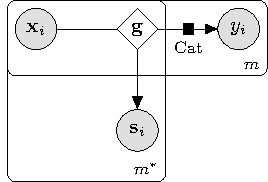
\includegraphics[width=0.35\textwidth]{results/privlearn/general_model}
\caption{Вероятностная модель в формате плоских нотаций.}
\label{fg:st:plate}
\end{figure}

На рис. \ref{fg:st:plate} показан вид вероятностной модели в графовой нотации, для произвольной функции $\mathbf{g}$. Для каждой реализации $\mathbf{g}$ соответсвующий блок требует уточнение. На рис \ref{fg:ex:synt:plate} показана более подробная реализация в случае, когда модель $\mathbf{g}$ это линейная модель.

Для задачи многоклассовой классификации рассматриваются следующие вероятностные предположения:
\begin{enumerate}
\label{st:class:1}
	\item рассматривается функция учителя $\mathbf{f}\in\mathfrak{F}_{\text{cl}}^{*}$ \eqref{eq:F:set:cl:priv};
	\item рассматривается функция ученика следующего вида $\mathbf{g}\in\mathfrak{G}_{\text{cl}}$ \eqref{eq:G:set:cl};
	\item для истинных меток рассматривается категориальное распределение $p\bigr(y|\mathbf{x}, \mathbf{g}\bigr) = \text{Cat}\bigr(\mathbf{g}\bigr(\mathbf{x}\bigr)\bigr)$, где $\mathbf{g}\bigr(\mathbf{x}\bigr)$ задает вероятность каждого класса;
	\item для меток учителя введем плотность распределения
\[
\label{reg:dist}
\begin{aligned}
	p\bigr(\mathbf{s}|\mathbf{x}, \mathbf{g}\bigr) = C\prod_{k=1}^{K}g_k\bigr(\mathbf{x}\bigr)^{s^k},
\end{aligned}
\]
где $g^k$ обозначает вероятность класса $k$, которую предсказывает модель ученика, а $s^k$ --- вероятность класса $k$, которую предсказывает модель учителя.
\end{enumerate}
\begin{theorem}
\label{theorem:st:dist}
Пусть вероятнось каждого класса отделима от нуля и единицы, то есть для всех $k$ выполняется $1 > 1- \varepsilon > g_k\bigr(\mathbf{x}\bigr) > \varepsilon > 0,$ тогда при
\[
C=\left(-1\right)^{K}\frac{K^{K/2}}{2^{K(K-1)/2}}\prod_{k=1}^{K}g_k\bigr(\mathbf{x}\bigr)\log g_k\bigr(\mathbf{x}\bigr)
\]
функция $p\bigr(\mathbf{s}|\mathbf{x}, \mathbf{g}\bigr)$ определенная в \eqref{reg:dist} является плотностью распределения.
\end{theorem}
\begin{proof}
	Во-первых покажем, что для произвольного вектора ответов $\mathbf{s} \in \mathcal{S}_K$ выполняется $p\bigr(\mathbf{s}|\mathbf{x}, \mathbf{g}\bigr) \geq 0$. Заметим, что для всех $k$ выполняется, что $\log g_k\bigr(\mathbf{x}\bigr) < 0,$ тогда
\[
\begin{aligned}
	C=\underbrace{\frac{K^{K/2}}{2^{K(K-1)/2}}}_{>0}\prod_{k=1}^{K}\underbrace{g_k\bigr(\mathbf{x}\bigr)}_{>\varepsilon}\underbrace{\left(-\log g_k\bigr(\mathbf{x}\bigr)\right)}_{>0} > 0,
\end{aligned}
\]
тогда с учетом того, что $g_k\bigr(\mathbf{x}\bigr) >0$ и $C>0$ получаем, что $p\bigr(\mathbf{s}|\mathbf{x}, \mathbf{g}\bigr) \geq 0$.
	Во-вторых покажем, что интеграл по всему пространству ответов $\mathcal{S}_K$ является конечным:
	\[
	\label{theorem:st:dist:eq:1}
	\begin{aligned}
		\int_{\mathcal{S}_K}p\bigr(\mathbf{s}|\mathbf{x}, \mathbf{g}\bigr)ds &= \int_{\mathcal{S}_K}\prod_{k=1}^{K}g_k\bigr(\mathbf{x}\bigr)^{s^k}ds = \prod_{k=1}^{K}\int_{\mathcal{S}_K}g_k\bigr(\mathbf{x}\bigr)^{s^k}ds\\ 
		& = \prod_{k=1}^{K}\int_{0}^{1}\frac{r^{K-1}\sqrt{K}}{\left(K-1\right)!\sqrt{2^{K-1}}}g_k\bigr(\mathbf{x}\bigr)^{r}dr = \prod_{k=1}^{K}\underbrace{\frac{\sqrt{K}}{\left(K-1\right)!\sqrt{2^{K-1}}}}_{D}\int_{0}^{1}r^{K-1}g_k\bigr(\mathbf{x}\bigr)^{r}dr \\
		& = D^K\prod_{k=1}^{K} \int_{0}^{1}r^{K-1}\exp\bigr(r\log g_k\bigr(\mathbf{x}\bigr)\bigr)dr \\
		& = \left(-D\right)^K\prod_{k=1}^{K}\log g_k\bigr(\mathbf{x}\bigr)\left(\Gamma\bigr(K\bigr) - \Gamma\bigr(K, -\log g_k\bigr(\mathbf{x}\bigr)\bigr)\right) \\
		& = \left(-D\right)^K\left(K-1\right)!^K\prod_{k=1}^{K}\log g_k\bigr(\mathbf{x}\bigr)\left(1 -g_k\bigr(\mathbf{x}\bigr) \exp_{K-1}\bigr(-\log g_k\bigr(\mathbf{x}\bigr)\bigr)+g_k\bigr(\mathbf{x}\bigr)\right) \\
		& = \frac{\left(-\sqrt{K}\right)^K}{2^{K(K-1)/2}}\prod_{k=1}^{K}\log g_k\bigr(\mathbf{x}\bigr)\left(1 -g_k\bigr(\mathbf{x}\bigr) \exp_{K-1}\bigr(-\log g_k\bigr(\mathbf{x}\bigr)\bigr)+g_k\bigr(\mathbf{x}\bigr)\right) < \infty,
	\end{aligned}
	\]
где $\Gamma\bigr(K\bigr)$ является гамма функцией, $\Gamma\bigr(K, -\log g_k\bigr(\mathbf{x}\bigr)\bigr)$ является неполной гамма функцией, $\exp_{n}\bigr(x\bigr)$ является суммой Тейлора из первых $n$ слагаемых. В рамках приближенных расчетов будем считать, что $\exp_{n}\bigr(x\bigr)\approx\exp\bigr(x\bigr),$ тогда с учетом \eqref{theorem:st:dist:eq:1} получаем:
	\[
	\label{theorem:st:dist:eq:2}
	\begin{aligned}
		C\bigr(\mathbf{g}, \mathbf{x}\bigr) = \int_{\mathcal{S}_K}p\bigr(\mathbf{s}|\mathbf{x}, \mathbf{g}\bigr)ds \approx \left(-1\right)^{K}\frac{K^{K/2}}{2^{K(K-1)/2}}\prod_{k=1}^{K}g_k\bigr(\mathbf{x}\bigr)\log g_k\bigr(\mathbf{x}\bigr)
	\end{aligned}
	\]
	
Полученное выражение \eqref{theorem:st:dist:eq:2} заканчивает доказательство теоремы.
\end{proof}

Из теоремы \ref{theorem:st:dist} следует, что плотность введенная для меток учителя является плотностью распределения, следовательно можно воспользоваться выражением \eqref{eq:st:12}.
Используя предположения 1)--4) и подставляя в \eqref{eq:st:12} получаем следующую оптимизационную задачу:
\[
\label{eq:st:class:1}
\begin{aligned}
\hat{\mathbf{g}} = \arg\max_{\mathbf{g}\in \mathcal{G}} & \sum_{i\not\in \mathcal{I}}\sum_{k=1}^{K}y_i^k\log g_k\bigr(\mathbf{x}_i\bigr)\bigr|_{T=1} \\
&+ \left(1-\lambda\right)\sum_{i\in \mathcal{I}}\sum_{k=1}^{K}y_i^k\log g_k\bigr(\mathbf{x}_i\bigr)\bigr|_{T=1} + \lambda\sum_{i\in \mathcal{I}}\sum_{k=1}^{K}s_{i,k}\log g_k\bigr(\mathbf{x}_i\bigr)\bigr|_{T=T_0} \\
&+ \lambda \sum_{i\in \mathcal{I}}\sum_{k=1}^{K}\left(\log g_k\bigr(\mathbf{x}_i\bigr)\bigr|_{T=T_0} + \log\log\frac{1}{g_k\bigr(\mathbf{x}_i\bigr)}\bigr|_{T=T_0}\right),
\end{aligned}
\]
где выражение $\cdot\bigr|_{T=t}$ обозначает, что в предыдущую функцию $\text{softmax}$ требуется подставить значение температуры $T$ равное некоторому значению $t$.

Проанализировав выражение \eqref{eq:st:class:1} получаем, что первые три слагаемые совпадают со слагаемыми в выражении \eqref{eq:hinton:1} при $\mathcal{I} = \{1, \cdots, m\},$ и $\lambda=\frac{1}{2}$, а третье слагаемое является некоторым регуляризатором, который получен из вида распределения.

Анализируя первые три слагаемых в выражении \eqref{eq:st:class:1} получаем, что при $T_0 = 1$ получаем сумму кросс энтропий между двумя распределениями для каждого объекта:
\begin{enumerate}
	\item первое распределение это выпуклая комбинация с весом $1-\lambda$ и $\lambda$: распределения задаваемое метками объектов $\text{Cat}\bigr(\mathbf{y}\bigr)$ и распределения задаваемого моделью учителя $\text{Cat}\bigr(\mathbf{s}\bigr)$
	\item второе распределение это распределение задаваемое плотностью распределения ответов ученика $\text{Cat}\bigr(\mathbf{g}\bigr(\mathbf{x}\bigr)\bigr)$.
\end{enumerate}
Получаем, что модель ученика восстанавливает плотность не исходных меток, а новую плотность, которая является выпуклой комбинаций плотности исходных меток и меток учителя.
Для задачи регрессии рассматриваются следующие вероятностные предположения:
\begin{enumerate}
	\item рассматривается функция учителя $\mathbf{f}\in\mathfrak{F}_{\text{rg}}^{*}$:
	\[
	\label{eq:F:set:priv}
	\begin{aligned}
	\mathfrak{F}_{\text{rg}}^* = \left\{\mathbf{f}| \mathbf{f} = \mathbf{v}^*\bigr(\mathbf{x}^*\bigr), \quad \mathbf{v}^*: \mathbb{R}^{n^*} \to \mathbb{R} \right\},
	\end{aligned}
	\]
	где $\mathbf{v}^*$ --- это дифференцируемая параметрическая функция;
	\item рассматривается функция ученика $\mathbf{g}\in\mathfrak{G}_{\text{rg}}$:
\[
\label{eq:G:set:rg}
\mathfrak{G}_{\text{rg}} = \left\{\mathbf{g}| \mathbf{g} = \mathbf{z}\bigr(\mathbf{x}\bigr), \quad \mathbf{z}: \mathbb{R}^n \to \mathbb{R}^K \right\},
\]
где $\mathbf{z}$ --- это дифференцируемая параметрическая функция;
	\item истинные метки имеют нормальное распределение
	\[
		p\bigr(y|\mathbf{x}, \mathbf{g}\bigr) = \mathcal{N}\bigr(y|\mathbf{g}\bigr(\mathbf{x}\bigr), \sigma\bigr);
	\]
	\item метки учителя распределены
	\[
		p\bigr(s| \mathbf{x}, \mathbf{g}\bigr) = \mathcal{N}\bigr(s|\mathbf{g}\bigr(\mathbf{x}\bigr), \sigma_s\bigr);
	\]
\end{enumerate}

Используя предположения 1)--4) и подставляя в \eqref{eq:st:12} получаем следующую оптимизационную задачу:
\[
\label{eq:st:reg:1}
\begin{aligned}
\hat{g} = \arg\min_{g\in \mathcal{G}} & \sum_{i\not\in \mathcal{I}}\sigma^2\left(y_i-\mathbf{g}\bigr(\mathbf{x}_i\bigr)\right)^2 \\
&+ \left(1-\lambda\right)\sum_{i\in \mathcal{I}}\sigma^2\left(y_i-\mathbf{g}\bigr(\mathbf{x}_i\bigr)\right)^2 + \lambda\sum_{i\in \mathcal{I}}\sigma_s^2\left(s_i-\mathbf{g}\bigr(\mathbf{x}_i\bigr)\right)^2.
\end{aligned}
\]
Выражение \eqref{eq:st:reg:1} записано с точностью до аддитивной константы относительно $\mathbf{g}$. 

\begin{theorem}
\label{theorem:st:reg}
Пусть множество $\mathcal{G}$ описывает класс линейных функций вида $\mathbf{g}\bigr(\mathbf{x}\bigr) = \mathbf{w}^{\mathsf{T}}\mathbf{x}.$ Тогда решение оптимизационной задачи \eqref{eq:st:reg:1} эквивалентно решению следующей задачи линейной регрессии:
\[
\label{eq:st:reg:th:st:1}
\begin{aligned}
\mathbf{y''} = \mathbf{X}\mathbf{w} + \bm{\varepsilon}, \bm{\varepsilon} \sim \mathcal{N}\bigr(\mathbf{0}, \bm{\Sigma}\bigr),
\end{aligned}
\]
где $\bm{\Sigma}^{-1}=\text{diag}\bigr(\bm{\sigma'}\bigr)$ и $\mathbf{y''}$ имеют следующий вид:
\[
\label{eq:st:reg:th:st:2}
\begin{aligned}
\sigma'_{i} &= \begin{cases}
\sigma^2, \text{если} i \not \in \mathcal{I}\\
\left(1-\lambda\right)\sigma^2+\lambda\sigma_s^2, \text{иначе}\\
\end{cases}, \\
\mathbf{y''} &= \bm{\Sigma}\mathbf{y'},\\
y'_i &= \begin{cases}
\sigma^2y_i, \text{если} i \not \in \mathcal{I}\\
\left(1-\lambda\right)\sigma^2y_i+\lambda\sigma_s^2s_i, \text{иначе}\\
\end{cases}.
\end{aligned}
\]
\end{theorem}
\begin{proof}
Обозначеним $\mathbf{a}_{\mathcal{J}} = [a_i| i \in \mathcal{J}]^{\mathsf{T}},$ где $\mathbf{a}$ произвольный вектор, а $\mathcal{J}$ произвольное не пустое индексное множество. Подвектор вектора ответов $\mathbf{y}$, для элементов которого доступна привилегированная информация обозначим $\mathbf{y}_{\mathcal{I}} = [y_i| i \in \mathcal{I}]^{\mathsf{T}}$. Аналогично обозначим матрицу $\mathbf{X}_\mathcal{I}=[\mathbf{x}_{i}| i \in \mathcal{I}]^{\mathsf{T}}$.

В случае линейной модели $\mathbf{g}\bigr(\mathbf{x}\bigr) = \mathbf{w}^{\mathsf{T}}\mathbf{x}$ выражение \eqref{eq:st:reg:1} принимает вид:
\[
\label{eq:st:reg:2}
\begin{aligned}
\hat{\mathbf{w}} = \arg\min_{\mathbf{w}\in \mathcal{W}} &  \sigma^2\left(\mathbf{y}_{\bar{\mathcal{I}}}-\mathbf{X}_{\bar{\mathcal{I}}}\mathbf{w}\right)^{\mathsf{T}}\left(\mathbf{y}_{\bar{\mathcal{I}}}-\mathbf{X}_{\bar{\mathcal{I}}}\mathbf{w}\right) \\
&+ \sigma^2\left(1-\lambda\right)\left(\mathbf{y}_{\mathcal{I}}-\mathbf{X}_{\mathcal{I}}\mathbf{w}\right)^{\mathsf{T}}\left(\mathbf{y}_{\mathcal{I}}-\mathbf{X}_{\mathcal{I}}\mathbf{w}\right) + \sigma^2_s\lambda\left(\mathbf{s}_{\mathcal{I}}-\mathbf{X}_{\mathcal{I}}\mathbf{w}\right)^{\mathsf{T}}\left(\mathbf{s}_{\mathcal{I}}-\mathbf{X}_{\mathcal{I}}\mathbf{w}\right).
\end{aligned}
\]

Раскроем скобки и сгруппируем:
\[
\label{eq:st:reg:3}
\begin{aligned}
\hat{\mathbf{w}} = \arg\min_{\mathbf{w}\in \mathcal{W}} &  \sigma^2\left(\mathbf{w}^{\mathsf{T}}\mathbf{X}^{\mathsf{T}}_{\bar{\mathcal{I}}}\mathbf{X}_{\bar{\mathcal{I}}}\mathbf{w} - 2\mathbf{y}^{\mathsf{T}}_{\bar{\mathcal{I}}}\mathbf{X}_{\bar{\mathcal{I}}}\mathbf{w}\right) \\
&+ \left(1-\lambda\right)\sigma^2\left(\mathbf{w}^{\mathsf{T}}\mathbf{X}^{\mathsf{T}}_{\mathcal{I}}\mathbf{X}_{\mathcal{I}}\mathbf{w}- 2\mathbf{y}^{\mathsf{T}}_{\mathcal{I}}\mathbf{X}_{\mathcal{I}}\mathbf{w}\right) + \lambda\sigma^2_s\left(\mathbf{w}^{\mathsf{T}}\mathbf{X}^{\mathsf{T}}_{\mathcal{I}}\mathbf{X}_{\mathcal{I}}\mathbf{w}- 2\mathbf{s}^{\mathsf{T}}_{\mathcal{I}}\mathbf{X}_{\mathcal{I}}\mathbf{w}\right)
\end{aligned}
\]
Продифференцируем выражение, приравняем к нулю и сгруппируем элементы:
\[
\label{eq:st:reg:4}
\begin{aligned}
\left(\sigma^{2}\mathbf{X}^{\mathsf{T}}_{\bar{\mathcal{I}}}\mathbf{X}_{\bar{\mathcal{I}}} + \left(1-\lambda\right)\sigma^2\mathbf{X}^{\mathsf{T}}_{\mathcal{I}}\mathbf{X}_{\mathcal{I}} + \lambda\sigma^{2}_s\mathbf{X}^{\mathsf{T}}_{\mathcal{I}}\mathbf{X}_{\mathcal{I}}\right) \mathbf{w} =& 2\sigma^2\mathbf{X}^{\mathsf{T}}_{\bar{\mathcal{I}}}\mathbf{y}_{\bar{\mathcal{I}}} \\
&+ 2\left(1-\lambda\right)\sigma^2\mathbf{X}^{\mathsf{T}}_{\mathcal{I}}\mathbf{y}_{\mathcal{I}} + 2\lambda\sigma_s^2\mathbf{X}^{\mathsf{T}}_{\mathcal{I}}\mathbf{s}_{\mathcal{I}}.
\end{aligned}
\]
Воспользуемся следующими равенствами:
\[
\label{eq:st:reg:simp}
\begin{aligned}
\sigma^{2}\mathbf{X}^{\mathsf{T}}_{\bar{\mathcal{I}}}\mathbf{X}_{\bar{\mathcal{I}}} + \left(1-\lambda\right)\sigma^2\mathbf{X}^{\mathsf{T}}_{\mathcal{I}}\mathbf{X}_{\mathcal{I}} + \lambda\sigma^{2}_s\mathbf{X}^{\mathsf{T}}_{\mathcal{I}}\mathbf{X}_{\mathcal{I}} &= \mathbf{X}^{\mathsf{T}}\bm{\Sigma}^{-1}\mathbf{X},\\
2\sigma^2\mathbf{X}^{\mathsf{T}}_{\bar{\mathcal{I}}}\mathbf{y}_{\bar{\mathcal{I}}} + 2\left(1-\lambda\right)\sigma^2\mathbf{X}^{\mathsf{T}}_{\mathcal{I}}\mathbf{y}_{\mathcal{I}} + 2\lambda\sigma_s^2\mathbf{X}^{\mathsf{T}}_{\mathcal{I}}\mathbf{s}_{\mathcal{I}} &= 2\mathbf{X}\mathbf{y'},
\end{aligned}
\]
где $\bm{\Sigma}$ и $\mathbf{y'}$ из условия задачи \eqref{eq:st:reg:th:st:2}.

Подставляя \eqref{eq:st:reg:simp} в \eqref{eq:st:reg:4} получаем:
\[
\label{eq:st:reg:5}
\begin{aligned}
\mathbf{w} = 2\left(\mathbf{X}^{\mathsf{T}}\bm{\Sigma}^{-1}\mathbf{X}\right)^{-1}\mathbf{X}\bm{\Sigma}^{-1}\mathbf{y''},
\end{aligned}
\]
что соответсвует решению задачи \eqref{eq:st:reg:th:st:1}.
\end{proof}

Теорема \ref{theorem:st:reg} показывает, что обучения с учителем для задачи регрессии можно свести к классической задачи оптимизации для задачи линейной регрессии.

\section{Анализ вероятностного подхода к дистилляции моделей линейных моделей}
Проводится вычислительный эксперимент для анализа качества моделей, которые получены путем дистилляции модели учителя в модель ученика. Как показано в теореме \ref{theorem:st:reg} задачу регрессии с учителем можно свести к задачи регрессии без учителя, поэтому в эксперименте более подробно рассматривается случай классификации. Во всех частях вычислительного эксперимента для поиска оптимальных параметров нейросетей использовался градиентный метод оптимизации Адам \cite{kingma2014}.

В данной части проводится эксперимент для задачи классификации для выборки FashionMNIST \cite{fashionmnist}. В качестве модели учителя $\mathbf{f}$ рассматривается модель нейросети с двумя сверточными слоями и с тремя полносвязными слоями, в качестве функции активации рассматривается ReLu. Модель учителя содержит $ 30$ тысяч обучаемых параметров. В качестве модели ученика рассматривается модель логистической регрессии для многоклассовой классификации. Модель ученика содержит $7850$ обучаемых параметров.

\begin{figure}[h!t]\center
\includegraphics[width=1\textwidth]{results/privlearn/mnist_loss}
\caption{Зависимость кросс--этропии между истинными метками и предсказанными учеников вероятностями классов: a) на обучающей выборке; b) на тестовой выборке.}
\label{fg:ex:fashionmnist:loss}
\end{figure}

На рис. \ref{fg:ex:fashionmnist:loss} показан график зависимости кросс--энтропии между истинными метками объектов и вероятностями, которые предсказывает модель ученика. На графике сравнивается моделя, которая обучалась без учителя (в задаче оптимизации \eqref{eq:st:class:1} присутствует только первое слагаемое) с моделью, которая была получена путем дистилляции модели нейросети в линейную модель. На графике видно, что обе модели начинают переобучатся после 30-й итерации, но модель, которая получена путем дистилляции переобувается не так быстро, что следует из того, что ошибка на тестовой выборке растет медленней, а на обучающей выборке падает также медленней.


Проанализируем модель на синтетической выборке. Выборка построенная следующим образом:
\[
\begin{aligned}
\mathbf{W} &= \left[\mathcal{N}\bigr(w_{jk}|0, 1\bigr)\right]_{n\times K}, \quad &\mathbf{X} &= \left[\mathcal{N}\bigr(x_{ij}|0, 1\bigr)\right]_{m\times n}, \\
 \mathbf{S} &= \text{softmax}\left(\mathbf{XW}\right), \quad &\mathbf{y} &= \left[\text{Cat}\bigr(y_i| \mathbf{s}_i\bigr)\right],
\end{aligned}
\]
где функция $\text{softmax}$ берется построчно. Строки матрицы $\mathbf{S}$ будем рассматривать как предсказание учителя, то есть учитель знает истинные вероятности каждого класса. На рис. \ref{fg:ex:synt:plate} показана вероятностная модель в графовой нотации. В эксперименте число признаков $n=10$, число классов $K=3$, для обучения было сгенерировано $m_{\text{train}}=1000$ и $m_{\text{test}}=100$ объектов.

На рис. \ref{fg:ex:synt:distr:real} показано распределение по классам для каждого объекта обучающей выборки. Видно, что все классы являются равновероятными.

Построим в качестве ученика простую линейную модель, которая минимизирует крос--энтропийную (первое слагаемое в формуле \eqref{eq:st:class:1}). Представление данной модели в виде графовой модели показано на рис. \ref{fg:ex:synt:plate}.

\begin{figure}[h!t]\center
\includegraphics[width=0.35\textwidth]{results/privlearn/linear_model}
\caption{Вероятностная модель используемая в синтетическом эксперименте.}
\label{fg:ex:synt:plate}
\end{figure}

\begin{figure}[h!t]\center
\includegraphics[width=1\textwidth]{results/privlearn/syn_real_distr}
\caption{Истинное распределение  объектов по классам.}
\label{fg:ex:synt:distr:real}
\end{figure}


На рис. \ref{fg:ex:synt:distr:without} показано распределение вероятностей классов, которое предсказала модель. Видно, что данное распределение является не соответствует истинному, так как модель сосредотачивает всю вероятность в одном классе.

\begin{figure}[h!t]\center
\includegraphics[width=1\textwidth]{results/privlearn/syn_without_teacher_distr}
\caption{Распределение предсказанное моделью без использования информации об истинном распределение на классах.}
\label{fg:ex:synt:distr:without}
\end{figure}

\begin{figure}[h!t]\center
\includegraphics[width=1\textwidth]{results/privlearn/syn_with_teacher_distr}
\caption{Распределение предсказанное моделью c использования информации об истинном распределение на классах.}
\label{fg:ex:synt:distr:with}
\end{figure}

\begin{figure}[h!t]\center
\includegraphics[width=1\textwidth]{results/privlearn/syn_T_lambda}
\caption{Вероятности классов для разных объектов.}
\label{fg:ex:synt:distr:lambda_T}
\end{figure}

Рассмотрим модель, которая учитывает информацию о истинных распределениях на классах для каждого объекта. Для этого будем минимизировать первые три слагаемых в формуле \eqref{eq:st:class:1}, при $T_0=1$ и $\lambda=0{,}75$. В качестве меток учителя $s_{i,k}$ использовались истинные вероятности для каждого класса для данного объекта. На рис \ref{fg:ex:synt:distr:with} показано распределение, которое дала модель в данном случае, видно, что распределения являются сглаженными и концентрации всей вероятности в одном классе не наблюдается.

Заметим, что в данном примере предполагается, что модель учителя учитывает не только метки классов, а и распределение на метках классов, в то время как в выборке $\mathcal{D} = \{\mathbf{X}, \mathbf{y}\},$ имеются только точечные оценки в виде меткок. 

В данном примере используются истинные распределения в качестве предсказаний учителя, но их можно заменить предсказаниями модели учителя, которая предсказывает не только сами меток, а и их распределение для каждого объекта.

На рис. \ref{fg:ex:synt:distr:lambda_T} показана зависимость вероятности верного класса от температуры $T$ и параметра доверия $\lambda$ для одного из объекта из тестовой выборке. Видно, что при увеличении темпертуры распределение на классас становится более равномерным.

В данной части проводится эксперимент на выборке Twitter Sentiment Analysis. Данная выборка содержит короткие сообщения, для которых нужно предсказать эмоциональный окрас: содержит твит позитивный окрас или негативный. Выборка разделена на $1{,}18$ миллиона твитов для обучения и $0{,}35$ миллиона твитов для тестирования. В твитах была выполнена следующая предобработка:
\begin{itemize}
	\item все твиты были переведены в нижний регистр;
	\item все никнеймы вида ``@andrey'' были заменены на токен ``name'';
	\item все цифры были заменены на токен ``number''.
\end{itemize}
Результаты данной части эксперимента показаны в табл. \ref{tb:ce:1}. В качестве модели учителя использовалась модель Bi-LSTM с $170$ тысячами параметров для обучения. В качестве эмбедингов обучалась матрица из $30$ миллионов параметров в единой процедуре с моделью BI-LSTM. Обученная модель предсказывает с точностью $0{,}835$. В качестве модели ученика рассматривается модель с $1538$ параметрами, но в качестве эмбедингов рассматривается переобученная модель BERT.

\begin{table}[]
\caption{Сводная таблица результатов вычислительного эксперимента.}
\label{tb:ce:1}
\begin{center}
\begin{tabular}{|l|l|c|c|c|}
\hline
\multicolumn{1}{|c|}{Dataset} & \multicolumn{1}{c|}{Model} & CrossEntropyLoss      & Accuracy    &   StudentSize   \\ \hline
\multirow{2}{*}{FashionMnist} & without teacher    &  $0{,}461 \pm 0{,}005$ & $0{,}841\pm 0{,}002$ & 7850 \\ \cline{2-5} 
                              & with teacher       & $0{,}453 \pm 0{,}003$ & $0{,}842 \pm 0{,}002$ & 7850\\ \hline
\multirow{2}{*}{Synthetic}    & without teacher    & $0{,}225 \pm 0{,}002$ & $0{,}831\pm 0{,}002$ & 33 \\ \cline{2-5} 
                              &  with teacher       & $0{,}452 \pm 0{,}001$   & $0{,}828\pm 0{,}001$ & 33 \\ \hline
\multirow{2}{*}{Twitter }    & without teacher    & $0{,}501 \pm 0{,}006$ & $0{,}747\pm 0{,}005$ & $1538$  \\ \cline{2-5} 
                              &with teacher       & $0{,}489 \pm 0{,}003$   & $0{,}764\pm 0{,}004$ & $1538$ \\ \hline
\end{tabular}
\end{center}
\end{table}


\clearpage
\chapter{Байесовская дистилляция моделей глубокого обучения}
Исследуется проблема снижения числа обучаемых параметров моделей машинного обучения. Примерами таких моделей, с избыточным число параметров, являются AlexNet \cite{Krizhevsky2012}, VGGNet \cite{Simonyan2014}, ResNet \cite{Kaiming2015}, BERT \cite{Devlin2018, Vaswani2017}, mT5 \cite{Linting2021}, GPT3\cite{Brown2020} и другие.
\begin{table}[h!]
\caption{Число параметров в моделях машинного обучения.}
\label{tb:intro:1}
\begin{center}
\resizebox{\textwidth}{!}{
\begin{tabular}{|l|l|l|l|l|l|l|}
\hline
Название               & AlexNet     & VGGNet      & ResNet      & BERT     & mT5   & GPT3  \\ \hline
Год                          & 2012        & 2014        & 2015        & 2018     & 2020  & 2020  \\ \hline
Тип данных             & изображение & изображение & изображение & текст    & текст & текст \\ \hline
Число параметров, млрд & $0{,}06$    & $0{,}13$    & $0{,}06$    & $0{,}34$ & $13$  & $175$ \\ \hline
\end{tabular}
}
\end{center}
\end{table}
Табл. \ref{tb:intro:1} описывает глубокие модели машинного обучения.
Число параметров моделей машинного обучения с годами растет.
Это влечет снижение интерпретируемости моделей.
Данная проблема рассматривается в специальном классе задач по состязательным атакам (англ. adversarial attack) \cite{Zheng2020}.
Большое число параметров требует больших вычислительных ресурсов.
Из-за этого данные модели не могут быть использованы в мобильных устройствах.
Для снижения числа параметров предложен метод дистилляции модели \cite{Hinton2015, Vapnik2015, Lopez2016}.
Дистиллируемая модель с большим числом параметров называется \textit{учитель}, а модель получаемая путем дистилляции называется \textit{ученик}.
При оптимизации параметров модели ученика используется модель учителя с фиксированными параметрами.
\begin{definition}
Дистилляция модели --- снижение сложности модели путем выбора модели в множестве более простых моделей на основе параметров и ответов более сложной фиксированной модели.
\end{definition}

Идея дистилляции предложена в работах Дж.\,Е. Хинтона и В.\,Н. Вапником \cite{Hinton2015, Vapnik2015, Lopez2016}. В этих работах предлагается использовать ответы учителя в качестве целевой переменной для обучения модели ученика.
Поставлен ряд экспериментов, в которых проводилась дистилляция моделей для задачи классификации машинного обучения.
Базовый эксперимент на выборке MNIST \cite{mnist} показал применимость метода для дистилляции избыточно сложной нейросетевой модели в нейросетевую модель меньшей сложности.
Эксперимент по дистилляции ансамбля моделей в одну модель для решения задачи распознания речи. Также в работе \cite{Hinton2015} был проведен эксперимент по обучению экспертных моделей на основе одной модели с большим числом параметров при помощи предложенного метода дистилляции на ответах учителя.

В работе \cite{Zehao2017} предложен метод передачи селективности нейронов (англ. neuron selectivity transfer) основаный на минимизации специальной функции потерь основаной на максимальном среднем отклонении (англ. maximum mean discrepancy) между выходами всех слоев модели учителя и ученика. Вычислительный эксперимент показал эффективность данного метода для задачи классификации изображений на примере выборок CIFAR \cite{cifar10} и ImageNet \cite{imagenet}.

В данной работе предлагается метод,ы основанный на байесовском выводе.
В качестве априорного распределения параметров модели ученика предлагается использовать апостериорное распределение параметров модели учителя.
Решается задача сопоставления пространства параметров модели учителя и модели ученика.
Авторы предлагают подход, основаный на последовательном сопоставлении пространств параметров модели ученика и учителя. 
\begin{definition}
\label{def:structure}
Структура модели --- множество структурных параметров модели, которые задают вид суперпозиции.
\end{definition}
\begin{definition}
\label{def:sopos}
Сопоставление параметрических моделей --- изменение структуры модели (одной или нескольких моделей) в результате которого векторы параметров различных моделей лежат в одном пространстве.
\end{definition}
В результате сопоставления, параметры модели учителя и модели ученика лежат в одном пространстве.
Как следствие, в качестве априорного распределения параметров модели ученика выбирается апостериорное распределение параметров модели учителя.
В данной работе в качестве параметрических моделей рассматривается полносвязная нейронная сеть.
В качестве структурных параметров модели выбраны число слоев, а также размер каждого скрытого слоя.

В рамках предложенного метода сопоставления параметрических моделей не оговорен выбор порядка на множестве параметров модели учителя.
Для этого предлагается упорядочивать параметры модели учителя на основе их значимости.
Первый нейрон является наиболее значимым, а последний нейрон наименее значимым.
Порядок задается на основе отношения плотности распределения упорядочивваемого параметра к плотности распределения параметра в нуле \cite{graves2011} или на основе метода Белсли \cite{grabovoy2019}.
В рамках данной работы порядок на параметрах в рамках одного слоя задается случайный образом.

В рамках вычислительного эксперимента проводится теоретический анализ. Предложенный метод дистилляции анализируется на примере синтетической выборки, а также на реальной выборке FashionMnist \cite{fashionmnist}.

\section{Постановка задачи дистилляции в терминах байесовского подхода}
Задана выборка
\[
\label{eq:st:1}
\begin{aligned}
\mathfrak{D} = \left\{\left(\mathbf{x}_i, y_i\right)\right\}_{i=1}^{m}, \qquad \mathbf{x}_i \in \mathbb{R}^{n}, \quad y_i \in \mathbb{Y},
\end{aligned}
\]
где $\mathbf{x}_i, y_i$ --- признаковое описание и целевая переменная $i$-го объекта, число объектов в обучающей выборке обозначается $m$. Размер признакового описания объектов обозначается $n$. Множество $\mathbb{Y}=\{1,\cdots,K\}$ для задачи классификации, где $K$ число классов, множество $\mathbb{Y}=\mathbb{R}$ для задачи регрессии.

Задана модель учителя в виде суперпозиций линейных и нелинейных преобразований:
\[
\label{eq:st:2}
\begin{aligned}
f = \bm{\sigma} \circ \mathbf{U}_T \bm{\sigma} \circ \mathbf{U}_{T-1}\circ \cdots  \mathbf{U}_2\bm{\sigma} \circ \mathbf{U}_1,
\end{aligned}
\]
где $T$ --- число слоев модели учителя, $\bm{\sigma}$ --- функция активации, а $\mathbf{U}_t$ обозначает матрицу линейного преобразования. Матрицы $\mathbf{U}$ соединяются в вектор параметров $\mathbf{u}$ модели учителя $f$:
\[
\label{eq:st:2.1}
\begin{aligned}
\mathbf{u} = \text{vec}\bigr(\left[\mathbf{U}_T, \mathbf{U}_{T-1}, \cdots \mathbf{U}_1\right]\bigr),
\end{aligned}
\]
где $\text{vec}$ операция векторизации соединенных матриц.
Каждая матрица $\mathbf{U}_t$ имеет размер $n_t\times n_{t-1},$ где $n_0=n,$ а  $n_T={1}$ для задачи регрессии и $n_T=K$ для задачи классификации на $K$ классов. Число параметров $N_{\text{tr}}$ учителя $f$
\[
\label{eq:st:2.2}
\begin{aligned}
N_{\text{tr}} = \sum_{t=1}^{T}n_tn_{t-1}.
\end{aligned}
\]
Для построения вектора параметров $\mathbf{u}$ задается полный порядок на элементов матриц $\mathbf{U}_t$. Для полносвязнной нейронной сети вводится естественный порядок, индуцированный номером слоя $t$, номером нейрона, и номером элемента вектора параметров нейрона: выбирается матрица $\mathbf{U}_t$, строка этой матрицы и элемент строки.

Например, для модели учителя в задаче регрессии:
\[
\label{eq:st:3}
\begin{aligned}
f\bigr(\mathbf{x}\bigr) = \bm{\sigma} \circ \mathbf{U}_3 \bm{\sigma} \circ \mathbf{U}_2\bm{\sigma}\circ \mathbf{U}_1\mathbf{x},
\end{aligned}
\]
вектор параметров $\mathbf{u}$ принимает ви
\[
\label{eq:st:4}
\begin{aligned}
\mathbf{u} = \bigr[u_1^{1,1}, \cdots, u_1^{1,n},
                                               \cdots, 
                             u_1^{n_1,1}, \cdots, u_1^{n_1,n},  
                             u_2^{1, 1}, \cdots, u_2^{1, n_1}, 
                                                \cdots, 
                            u_2^{n_2, 1}, \cdots, u_2^{n_2, n_1},
                            u_3^{1, 1}, \cdots, u_3^{1, n_2}\bigr].
\end{aligned}
\]
Пусть для вектора параметров учителя $f$ известно апостериорное распределение параметров $p\bigr(\mathbf{u}|\mathfrak{D}\bigr)$. 
На основе выборки $\mathfrak{D}$ и апостериорного распределения параметров учителя $f$ требуется выбрать модель ученика из параметрического семейства функций:
\[
\label{eq:st:5}
\begin{aligned}
g = \bm{\sigma} \circ \mathbf{W}_L\bm{\sigma}  \circ \cdots \circ \mathbf{W}_1, \quad \mathbf{W}_l \in \mathbb{R}^{n_l \times n_{l-1}},
\end{aligned}
\]
где $L$ число слоев модели ученика.
Число параметров $N_{\text{st}}$ модели ученика $g$ вычисляется аналогично выражению \eqref{eq:st:2.2}.
Вектор параметров модели ученика $\mathbf{w}$ строится аналогичным образом \eqref{eq:st:2.1}.
Модель $g$ задается своим вектором параметров $\mathbf{w}$.
Следовательно, задача выбора модели $g$ эквивалентна задаче оптимизации вектора параметров $\mathbf{w}\in\mathbb{R}^{N_{\text{st}}}$.

Параметры $\hat{\mathbf{w}} \in \mathbb{R}^{N_{\text{st}}}$ оптимизируются при помощи вариационного вывода на основе совместного правдоподобия модели и данных:
\[
\label{eq:st:6}
\begin{aligned}
\mathcal{L}\bigr(\mathfrak{D}, \mathbf{A}\bigr) = \log p\bigr(\mathfrak{D}|\mathbf{A}\bigr) = \log \int_{\mathbf{w} \in \mathbb{R}^{N_{\text{st}}}}p\bigr(\mathfrak{D}|\mathbf{w}\bigr)p\bigr(\mathbf{w}|\mathbf{A}\bigr)d\mathbf{w},
\end{aligned}
\]
где $p\bigr(\mathbf{w}| \mathbf{A}\bigr)$ --- априорное распределение вектора параметров модели ученика.
Так как взятие интеграла \eqref{eq:st:6} является вычислительно сложной задачей, используется вариационный подход \cite{graves2011, grabovoy2019}. Для этого задается вариационное распределение параметров модели ученика $q\bigr(\mathbf{w}|\bm{\mu}, \bm{\Sigma}\bigr),$ которое аппроксимирует неизвестное апостериорное распределение $p\bigr(\mathbf{w}|\mathfrak{D}\bigr)$
\[
\label{eq:st:new:1}
\begin{aligned}
q\bigr(\mathbf{w}|\bm{\mu}, \bm{\Sigma}\bigr) \approx  p\bigr(\mathbf{w}|\mathfrak{D}\bigr).
\end{aligned}
\]
Далее распределение $q\bigr(\mathbf{w}|\bm{\mu}, \bm{\Sigma}\bigr)$ обозначается просто $q\bigr(\mathbf{w}\bigr).$ Оптимизация параметров $\mathbf{w}$ сводится к решению  задачи:
\[
\label{eq:st:7}
\begin{aligned}
\hat{\mathbf{w}} = \arg \min_{\bm{\mu}, \bm{\Sigma}, \mathbf{w}} \text{D}_{\text{KL}}\bigr(q\bigr(\mathbf{w}|\bm{\mu}, \bm{\Sigma}\bigr)||p\bigr(\mathbf{w}|\mathbf{A}\bigr)\bigr) - \log p\bigr(\mathbf{y}|\mathbf{X}, \mathbf{w}\bigr).
\end{aligned}
\]
Выражение \eqref{eq:st:7} не учитывает параметры учителя $f$. Для использования информации о распределении параметов учителя предлагается рассмотреть параметры априорного распределения $p\bigr(\mathbf{w}|\mathbf{A}\bigr)$ как функцию от апостериорного распределения учителя $p\bigr(\mathbf{u}|\mathfrak{D}\bigr)$.

\section{Построение априорного распределения параметров ученика на основе параметров учителя}
Апостериорное распределение параметров модели учителя предполагается нормальным:
\[
\label{eq:ap:1}
\begin{aligned}
p\bigr(\mathbf{u}|\mathfrak{D}\bigr) = \mathcal{N}\bigr(\mathbf{m}, \bm{\Sigma}\bigr),
\end{aligned}
\]
где $\mathbf{m}$ и $\bm{\Sigma}$ параметры этого распределения. На основе параметров $\mathbf{m}$ и $\bm{\Sigma}$ требуется задать параметры $\mathbf{A}$ априорного распределения $p\bigr(\mathbf{w}|\mathbf{A}\bigr).$
В случае, когда структура моделей учителя и ученика задаются числом слоев и размером этих слоев, то возможны следующие варианты: 1) число слоев и размер каждого слоя совпадает; 2) число слоев совпадает, а размеры различаются; 3) не совпадает число слоев.

\paragraph{Учитель и ученик принадлежат одному семейству.}
\label{section:one:space}
Рассмотрим следующие условия:
\begin{enumerate}
    \item число слоев модели учителя равняется числу слоев модели ученика $L=T$;
    \item размеры соответствующих слоев совпадают, другими словами, для всех $t, l$ таких, что $t=l$ выполняется $n_l = n_t,$ где $n_t$ обозначает размер $t$-го слоя учителя, а $n_l$ размер $l$-го слоя ученика.
\end{enumerate}
В случае выполнения этих условий, априорное распределение параметров модели ученика приравнивается к апостериорному распределения параметров учителя $p\bigr(\mathbf{w}|\mathbf{A}\bigr) = p\bigr(\mathbf{u}|\mathfrak{D}\bigr)$.

\paragraph{Удаление нейрона в слое учителя.}
Проведем согласование модели учителя и модели ученика, согласно определению \ref{def:sopos} при помощи последовательных преобразований параметров $\mathbf{u}$. Рассмотрим преобразование:
\[
\label{eq:ap:2}
\begin{aligned}
\phi\bigr(t, \mathbf{u}\bigr) : \mathbb{R}^{N_{\text{tr}}} \to \mathbb{R}^{N_{\text{tr}}-2n_t}
\end{aligned}
\]
вектора $\mathbf{u},$ которое описывает удаление одного нейрона из $t$-го слоя учителя.
%Другими словами, преобразование $\phi\bigr(t\bigr)$ зануляет одну из строк матрицы $\mathbf{U}_t$. Заметим, что данное зануление влечет зануление соответствующего столбца матрицы $\mathbf{U}_{t+1}$.
Обозначим новый вектор параметров $\bm{\upsilon} =  \phi\bigr(t, \mathbf{u}\bigr),$ а элементы вектора, которые были удалены как $\bar{\bm{\upsilon}}.$ Заметим, что векторы $\bm{\upsilon}$ и $\bar{\bm{\upsilon}}$ являются случайными величинами. 
%Введем следующие обозначения:
%\[
%\label{eq:ap:def:1}
%\begin{aligned}
%\bm{\upsilon} _{0} = \mathsf{E}\bm{\upsilon} , \quad \bar{\bm{\upsilon}}_0 = \mathsf{E}\bar{\bm{\upsilon}}, \quad  \bm{\Sigma}_{\bm{\upsilon},\bm{\upsilon}} = \text{cov}\bigr(\bm{\upsilon},\bm{\upsilon}\bigr), \quad  \bm{\Sigma}_{\bm{\upsilon},\bar{\bm{\upsilon}}} = \text{cov}\bigr(\bm{\upsilon},\bar{\bm{\upsilon}}\bigr), \quad  \bm{\Sigma}_{\bar{\bm{\upsilon}},\bar{\bm{\upsilon}}} = \text{cov}\bigr(\bar{\bm{\upsilon}},\bar{\bm{\upsilon}}\bigr),\\
%\end{aligned}
%\]
%где $ \text{cov}\bigr(\bm{\upsilon},\bm{\upsilon}\bigr)$ обозначает ковариационную матрицу.
\begin{theorem}
\label{theorem:ap:neural}
Пусть выполняются следующие условия:
\begin{enumerate}
\item апостериорное распределение $p\bigr(\mathbf{u}|\mathfrak{D}\bigr)$ параметров модели учителя является нормальным распределением \eqref{eq:ap:1};
\item число слоев модели учителя равняется числу слоев модели ученика $L=T$;
\item размеры соответствующих слоев не совпадают, другими словами, для всех $t, l$ таких, что $t=l$ выполняется $n_t \leq n_l,$.
\end{enumerate}
Тогда апостериорное распределения параметров модели учителя $p\bigr(\bm{\upsilon}|\mathfrak{D}\bigr)$ также является нормальным распределением.
%\[
%\label{eq:ap:3}
%\begin{aligned}
%p\bigr(\bm{\upsilon}|\mathfrak{D}\bigr) = \mathcal{N}\bigr(\bm{\upsilon}_{0}+\bm{\Sigma}_{\bm{\upsilon},\bar{\bm{\upsilon}}}\bm{\Sigma}_{\bar{\bm{\upsilon}},\bar{\bm{\upsilon}}}^{-1}\left(\mathbf{0} - \bar{\bm{\upsilon}}\right), \bm{\Sigma}_{\bm{\upsilon},\bar{\bm{\upsilon}}}\bm{\Sigma}_{\bar{\bm{\upsilon}},\bar{\bm{\upsilon}}}^{-1}\bm{\Sigma}_{\bm{\upsilon},\bar{\bm{\upsilon}}}\bigr).
%\end{aligned}
%\]
\end{theorem}
\begin{proof}
Не уменьшая общности, пусть $\phi\bigr(t, \mathbf{u}\bigr)$ удаляет $j$-й нейрон в $t$-м слое, что является удалением $j$-й строки матрицы $\mathbf{U}_t$. Заметим, что удаление $j$-й строки матрицы $\mathbf{U}_t$ влечет удаление $j$-й компоненты вектора $z_{t+1}$, где
\[
\label{eq:ap:tr:neural:1}
\begin{aligned}
\mathbf{z}_{t} = \bm{\sigma} \circ \mathbf{U}_{t-1} \bm{\sigma} \circ \cdots  \mathbf{U}_2\bm{\sigma} \circ \mathbf{U}_1\mathbf{x}.
\end{aligned}
\]

Удаление $j$-й компоненты вектора $\mathbf{z}_{t+1}$ эквивалентно занулению $j$-го столбца матрицы $\mathbf{U}_{t+1}.$ Заметим, что тогда предсказание модели не зависит от параметров $j$-й строки матрицы $\mathbf{U}_t,$ а следовательно донными параметрами также можно пренебречь.

Найдем распределение вектора $\bm{\upsilon}.$ Для поиска распределения вектора параметров после зануления $j$-го столбца матрицы $\mathbf{U}_{t+1}$ воспользуемся формулой условной вероятности $p\bigr(\bar{\bm{\nu}}_1|\mathfrak{D}, \bm{\nu}_1=\mathbf{0}\bigr)$, а для удаления $j$-й строки матрицы $\mathbf{U}_{t}$ воспользуемся маргинализацией распределения $p\bigr(\bar{\bm{\nu}}_1|\mathfrak{D}, \bm{\nu}_1=\mathbf{0}\bigr)$. Обозначим зануляемые параметры модели как $\bm{\nu}_1,$ а удаляемые параметры как $\bm{\nu}_2.$ Также обозначим все параметры, которые не были занулены как $\bar{\bm{\nu}}_1 = [\bm{\upsilon}^{\mathsf{T}}, \bm{\nu}_2^{\mathsf{T}}].$ Итоговое распределение параметров принимает  вид:
\[
\label{eq:ap:tr:1:1}
\begin{aligned}
p\bigr(\bm{\upsilon}|\mathfrak{D}\bigr)  = \int_{\bm{\nu}_2}p\bigr(\bar{\bm{\nu}}_1|\mathfrak{D}, \bm{\nu}_1=\mathbf{0}\bigr) d\bm{\nu}_2.
\end{aligned}
\]

Из свойств нормального распределения следует, что распределение
\[
\label{eq:ap:tr:neural:2}
\begin{aligned}
p\bigr(\bar{\bm{\nu}}_1|\mathfrak{D}, \bm{\nu}_1=\mathbf{0}\bigr)
\end{aligned}
\]
также является нормальным распределением с параметрами $\bm{\mu}, \bm{\Xi}$:
\[
\label{eq:ap:tr:1:1}
\begin{aligned}
\bm{\mu} &= \mathbf{m}_{\bar{\bm{\nu}}_1}+\bm{\Sigma}_{\bar{\bm{\nu}}_1,\bm{\nu}_1} \bm{\Sigma}_{\bm{\nu}_1,\bm{\nu}_1}^{-1} \left(\mathbf{0} - \mathbf{m}_{\bm{\nu}_1}\right), \\
 \bm{\Xi} &= \bm{\Sigma}_{\bar{\bm{\nu}}_1,\bar{\bm{\nu}}_1} - \bm{\Sigma}_{\bar{\bm{\nu}}_1,\bm{\nu}_1} \bm{\Sigma}_{\bm{\nu}_1,\bm{\nu}_1}^{-1} \bm{\Sigma}_{\bar{\bm{\nu}}_1,\bm{\nu}_1},
\end{aligned}
\]
где введены обозначения $\mathbf{m}_{\bar{\bm{\nu}}_1}, \mathbf{m}_{\bm{\nu}_1}$ соответствует подвектору вектора $\mathbf{m},$ который относится к параметрам $\bar{\bm{\nu}}_1$ и $\bm{\nu}_1$ соответсвенно. Ковариационная матрица $\bm{\Sigma}_{\bar{\bm{\nu}}_1,\bm{\nu}_1}$ обозначает подматрицу матрицы $\bm{\Sigma},$ которая соответсвует ковариационной матрицей между параметрами $\bar{\bm{\nu}}_1$ и $\bm{\nu}_1.$

Распределение $p\bigr(\bm{\upsilon}|\mathfrak{D}\bigr)$ найдем при помощи маргинализации распределения \eqref{eq:ap:tr:neural:2} по параметрам $\bm{\nu}_2.$ Используя свойства нормального распределения получаем распределения:
\[
\label{eq:ap:3}
\begin{aligned}
p\bigr(\bm{\upsilon}|\mathfrak{D}\bigr) = \mathcal{N}\bigr(\bm{\mu}_{\bm{\upsilon}},  \bm{\Xi}_{\bm{\upsilon}, \bm{\upsilon}}\bigr),
\end{aligned}
\]
где $\bm{\mu}_{\bm{\upsilon}}$ обозначает подвектор вектора $\bm{\mu},$ который относится к параметру $\bm{\upsilon}$, а матрица $\bm{\Xi}_{\bm{\upsilon}, \bm{\upsilon}}$ является подматрицей матрицы $\bm{\Xi}$, которая относится к вектору параметрамов $\bm{\upsilon}.$
\end{proof}

Теорема \ref{theorem:ap:neural} задает апостериорное распределение параметров \eqref{eq:ap:3} после зануления нейронов в модели нейросети --- учителя. Заметим, что аналогичным образом можно удалить сразу подмножество нейронов в рамках одного слоя. В случае, если число нейронов отличается в нескольких слоях модели нейросети учителя, то выполняется последовательно применения отображения $\phi\bigr(t, \mathbf{u}\bigr)$ для каждого $t$-го слоя.

\paragraph{Удаление слоя учителя.}
%Пусть в модели учителя требуется убрать $t$-й слой. Рассмотрим следующие условия:
%\begin{enumerate}
 %   \item соответствующие размеры слоев совпадают, $n_t=n_{t-1}$;
  %  \item функция активации удовлетворяет следующему свойству $\bm{\sigma} \circ \bm{\sigma} = \bm{\sigma}$.
%\end{enumerate}
Проведем согласование модели учителя и модели ученика, согласно определению \ref{def:sopos} при помощи последовательных преобразований вектора параметров $\mathbf{u}$. Рассмотрим преобразование:
\[
\label{eq:ap:4}
\begin{aligned}
\psi\bigr(t, \mathbf{u}\bigr) : \mathbb{R}^{N_{\text{tr}}} \to \mathbb{R}^{N_{\text{tr}}-n_tn_{t-1}}
\end{aligned}
\]
вектора $\mathbf{u}$ которое описывает удаление одного $t$-го слоя.
Обозначим новый вектор параметров $\bm{\upsilon} = \psi\bigr(t, \mathbf{u}\bigr),$ а элементы вектора, которые были удалены как $\bar{\bm{\upsilon}}.$ 
%Другими словами, преобразования $\psi\bigr(t\bigr)$ превращает матрицу $\mathbf{U}_t$ в единичную матрицу $\mathbf{I}$. 
%Для отображения $\psi\bigr(t\bigr)$ введем аналогичные \eqref{eq:ap:def:1} обозначения $\bm{\upsilon}_{0}, \bar{\bm{\upsilon}}_0, \bm{\Sigma}_{\bm{\upsilon},\bm{\upsilon}}, \bm{\Sigma}_{\bm{\upsilon},\bar{\bm{\upsilon}}}, \bm{\Sigma}_{\bar{\bm{\upsilon}},\bar{\bm{\upsilon}}}.$

\begin{theorem}
\label{theorem:ap:layer}
Пусть выполняются следующие условия:
\begin{enumerate}
\item апостериорное распределение параметров $p\bigr(\mathbf{u}|\mathfrak{D}\bigr)$ модели учителя является нормальным распределением \eqref{eq:ap:1};
\item соответствующие размеры слоев совпадают, $n_t=n_{t-1},$ то есть матрица $\mathbf{U}_t$ является квадратной;
\item функция активации удовлетворяет свойству идемпотентности $\bm{\sigma} \circ \bm{\sigma} = \bm{\sigma}$.
\end{enumerate}
Тогда апостериорное распределения также описывается нормальным распределением со следующей плотностью распределения:
\[
\label{eq:ap:5}
\begin{aligned}
p\bigr(\bm{\upsilon}|\mathfrak{D}\bigr) = \mathcal{N}\bigr(\mathbf{m}_{\bm{\upsilon}}+\bm{\Sigma}_{\bm{\upsilon},\bar{\bm{\upsilon}}} \bm{\Sigma}_{\bar{\bm{\upsilon}},\bar{\bm{\upsilon}}}^{-1} \left(\mathbf{i} - \bar{\bm{\upsilon}}\right), \bm{\Sigma}_{\bm{\upsilon},\bm{\upsilon}} - \bm{\Sigma}_{\bm{\upsilon},\bar{\bm{\upsilon}}}\bm{\Sigma}_{\bar{\bm{\upsilon}},\bar{\bm{\upsilon}}}^{-1}\bm{\Sigma}_{\bm{\upsilon},\bar{\bm{\upsilon}}}\bigr),
\end{aligned}
\]
где вектор $\mathbf{i}$ задается следующим образом:
\[
\mathbf{i}=[\underbrace{1, 0, \cdots, 0}_{n_t}, \underbrace{0, 1, \cdots, 0}_{n_t}, \underbrace{0, 0, 1, \cdots, 0}_{n_t}, \underbrace{0, \cdots, 1}_{n_t}]^{\mathsf{T}}.
\]
\end{theorem}
\begin{proof}
Рассмотрим структуру нейронной сети с $T$ слоями и $T+1$ слоем. Не уменьшая общности для удаления рассматривается $t$-й слой, для которого выполняются условия этой теоремы. Заметим, что если $t$-й слой нейронной сети с $T+1$ слоем приравнять к единичной матрице, то он будет эквивалентным архитектуре с $T$ слоями:
\[
\label{eq:ap:tr:2:1}
\begin{aligned}
f &= \bm{\sigma} \circ \mathbf{U}_{T+1}\bm{\sigma} \circ \mathbf{U}_T \cdots \bm{\sigma} \circ \mathbf{U}_t\bm{\sigma} \circ \cdots  \mathbf{U}_2\bm{\sigma} \circ \mathbf{U}_1 =\\
&=  \bm{\sigma} \circ \mathbf{U}_{T+1}\bm{\sigma} \circ \mathbf{U}_T \cdots \bm{\sigma} \circ \mathbf{I}\bm{\sigma} \circ \cdots  \mathbf{U}_2\bm{\sigma} \circ \mathbf{U}_1 =\\
&=  \bm{\sigma} \circ \mathbf{U}_{T+1}\bm{\sigma} \circ \mathbf{U}_T \cdots \bm{\sigma} \circ \bm{\sigma} \circ \cdots  \mathbf{U}_2\bm{\sigma} \circ \mathbf{U}_1 =^{1}\\
&=^{1}  \bm{\sigma} \circ \mathbf{U}_{T+1}\bm{\sigma} \circ \mathbf{U}_T \cdots \bm{\sigma} \circ \cdots  \mathbf{U}_2\bm{\sigma} \circ \mathbf{U}_1.
\end{aligned}
\]
\footnotetext[1]{Выполняется в силу условия теоремы об идемпотентности функции активации.}
Получаем, что удаление $t$-го слоя нейросети эквивалентно приравнивают матрицы параметров $t$-го слоя к единичной матрице. Распределение параметров после приравнивая к единичной матрице вычисляется при помощи условного распределения. В силу общих свойств нормального распределения условное распределения также является нормальным распределением с параметрами $\bm{\mu}, \bm{\Xi}:$
\[
\label{eq:ap:tr:2:2}
\begin{aligned}
\bm{\mu} &= \mathbf{m}_{\bm{\upsilon}}+\bm{\Sigma}_{\bm{\upsilon},\bar{\bm{\upsilon}}} \bm{\Sigma}_{\bar{\bm{\upsilon}},\bar{\bm{\upsilon}}}^{-1} \left(\mathbf{i} - \bar{\bm{\upsilon}}\right), \\
\bm{\Xi} &= \bm{\Sigma}_{\bm{\upsilon},\bm{\upsilon}} - \bm{\Sigma}_{\bm{\upsilon},\bar{\bm{\upsilon}}}\bm{\Sigma}_{\bar{\bm{\upsilon}},\bar{\bm{\upsilon}}}^{-1}\bm{\Sigma}_{\bm{\upsilon},\bar{\bm{\upsilon}}}\bigr),
\end{aligned}
\]
где вектор $\mathbf{m}_{\bm{\upsilon}}$ является подвектором вектора $\mathbf{m}$ соответсвующий параметрам $\bm{\upsilon},$ а матрица $\bm{\Sigma}_{\bm{\upsilon},\bar{\bm{\upsilon}}}$ является подматрицей ковариационной матрицы $\bm{\Sigma}$ соответсвующий векторам параметров $\bm{\upsilon}$ и $\bar{\bm{\upsilon}}.$
\end{proof}

Теорема \ref{theorem:ap:layer} задает апостериорное распределение \eqref{eq:ap:5} параметров после удаления слоя нейросети. Полученное распределение $p\bigr(\bm{\upsilon}|\mathfrak{D}\bigr) $ является оценкой апостериорного распределения модели без одного слоя.

\paragraph{Выполнение последовательных преобразований.}
Преобразования $\phi, \psi$ согласовывают пространства параметров учителя $f$ и ученика $g$. После сопоставления параметрических моделей получаем, что параметры модели учителя и модели учителя принадлежат одному семейству \ref{section:one:space}.
%После сопоставления параметров в качестве априорного распределения параметров ученика $p\bigr(\mathbf{w}|\mathfrak{D}\bigr)$ рассматривается полученное апостериорное распределение параметров учителя $p\bigr(\mathbf{u}'|\mathfrak{D}\bigr)$. Получаем, следующее приближение априорного распределения:
%\[
%\label{eq:ap:6}
%\begin{aligned}
%p_g\bigr(\mathbf{w}|\mathfrak{D}\bigr) = p_{f'}\bigr(\mathbf{w}|\mathfrak{D}\bigr),
%\end{aligned}
%\]
%где данное априорное распределение используется для поиска оптимальных параметров модели ученика $\hat{\mathbf{w}}$ с помощью \eqref{eq:st:7}.

\section{Анализ качества байесовской дистилляции полносвязных нейронных сетей}
Проводится вычислительный эксперимент для анализа предложенного метода дистилляции на основе апостериорного распределения параметров модели учителя.

Проанализируем модель на синтетической выборке. Выборка построенная следующим образом:
\[
\label{eq:ex:1}
\begin{aligned}
\mathbf{w} &= \left[w_j: w_{j}\sim \mathcal{N}\bigr(0, 1\bigr)\right]_{n\times 1}, \quad \mathbf{X} &= \left[x_{ij}: x_{ij}\sim\mathcal{N}\bigr(0, 1\bigr)\right]_{m\times n}, \\
 \mathbf{y} &= \left[y_i: y_i \sim \mathcal{N}\bigr(\mathbf{x}_i^{\mathsf{T}}\mathbf{w}, \beta\bigr)\right]_{m \times 1},
\end{aligned}
\] 
где $\beta=0{,}1$ --- уровень шума в данных. В эксперименте число признаков $n=10$, для обучения и тестирования было сгенерировано $m_{\text{train}}=900$ и $m_{\text{test}}=124$ объекта.

В качестве модели учителя рассматривалась модель --- многослойный перцептрон с двумя скрытыми слоями \eqref{eq:st:3}. Матрицы линейных преобразований имеют размер:
\[
\label{eq:ex:2}
\begin{aligned}
\mathbf{U}_{1} \in \mathbb{R}^{100 \times 10}, \quad \mathbf{U}_{2} \in \mathbb{R}^{50 \times 100}, \quad \mathbf{U}_{3} \in \mathbb{R}^{1 \times 50}.
\end{aligned}
\]
В качестве функции активации была выбрана функция активации $\text{ReLu}$.
Модель учителя предварительно обучена на основе вариационного вывода \eqref{eq:st:7}, где в качестве априорного распределения параметров выбрано стандартное нормальное распределение.

В качестве модели ученика были выбраны две конфигурации. Первая конфигурация получается путем удаления нейронов в модели учителя:
\[
\label{eq:ex:3}
\begin{aligned}
g = \bm{\sigma} \circ \mathbf{W}_3\bm{\sigma} \circ \mathbf{W}_2\bm{\sigma} \circ \mathbf{W}_1,
\end{aligned}
\]
где $\bm{\sigma}$ является нелинейной функцией активации, а матрицы линейных преобразований имеют размер:
\[
\label{eq:ex:4}
\begin{aligned}
\mathbf{W}_{1} \in \mathbb{R}^{10 \times 10}, \quad \mathbf{W}_{2} \in \mathbb{R}^{10 \times 10},  \quad \mathbf{W}_{3} \in \mathbb{R}^{1 \times 10}.
\end{aligned}
\]
В качестве функции активации была выбрана функция активации $\text{ReLu}$.

\begin{figure}[h!]
\includegraphics[width=0.5\textwidth]{results/bayesdistil/synthetic_likelihood_3_layers.eps}
\includegraphics[width=0.5\textwidth]{results/bayesdistil/synthetic_D_KL_3_layers.eps}
\caption{Структура \eqref{eq:ex:3} модели ученика $g$. Слева: правдоподобие выборки в зависимости от номера итерации при обучении. Справа: KL--дивергенция между вариационным и априорным распределениями параметров модели.}
\label{exp:fig1}
\end{figure}

Рис. \ref{exp:fig1} сравнивает модели ученика, со структурой \eqref{eq:ex:3}. Представлено сравнение разных моделей: модель без дистилляции, где в качестве априорного распределения выбирается стандартное нормальное распределение (на легенде обозначается student); модель с частичной дистилляцией, где в качестве среднего значения параметров выбираются параметры согласно выражения \eqref{eq:ap:3}, а ковариационная матрица была приравнена к единичной матрицы (на легенде обозначается distil-student); модель с полной дистилляцией согласно выражения \eqref{eq:ap:3} (на легенде обозначается distil-student-all). Видно, что модели ученика, где в качестве априорного распределения выбраны распределения, основанные на апостериорном распределение учителя имеют большее правдоподобие, чем модель где в качестве априорного распределения выбрано стандартное нормальное. Также заметим, что использования параметра среднего из апостериорного распределения дает основной вклад при дистилляции, так как качество моделей distil-student и distil-student-all совпадает.

Вторая конфигурация получается путем удаления слоя модели учителя:
\[
\label{eq:ex:5}
\begin{aligned}
g = \bm{\sigma} \circ \mathbf{W}_2\bm{\sigma} \circ \mathbf{W}_1,
\end{aligned}
\]
где $\bm{\sigma}$ является нелинейной функцией активации, а матрицы линейных преобразований имеют размер:
\[
\label{eq:ex:6}
\begin{aligned}
\mathbf{W}_{1} \in \mathbb{R}^{1 \times 50}, \quad \mathbf{W}_{2} \in \mathbb{R}^{50 \times 10}.
\end{aligned}
\]
 В качестве функции активации была выбрана функция активации $\text{ReLu}$.

\begin{figure}[h!]
\includegraphics[width=0.5\textwidth]{results/bayesdistil/synthetic_likelihood_2_layers.eps}
\includegraphics[width=0.5\textwidth]{results/bayesdistil/synthetic_D_KL_2_layers.eps}
\caption{Структура \eqref{eq:ex:5} модели ученика $g$. Слева: правдоподобие выборки в зависимости от номера итерации при обучении. Справа: KL--дивергенция между вариационным и априорным распределениями параметров модели.}
\label{exp:fig2}
\end{figure}

Рис. \ref{exp:fig2} сравнивает модели ученика со структурой \eqref{eq:ex:5}. Аналогично рис. \ref{exp:fig1}, на рис. \ref{exp:fig2} представлено сравнение модели без дистилляции (student), модели с дистилляцией параметра среднего значение (distil-student) и модели с полной дистилляцией (distil-student-all). В рамках данного эксперимента, по дистилляции модели учителя в модель ученика с меньшим числом параметров получены результаты, которые подтверждают, что задание априорного распределения параметров ученика позволяет улучшить число итераций при выборе оптимальных параметров модели ученика.

В рамках данного эксперимента проводился анализ байесовского подхода к дистилляции на реальных данных.  В качестве реальных данных выбрана выборка FashionMnist \cite{fashionmnist} которая является задачей классификации изображений на 10 классов.

В качестве модели учителя рассматривалась модель многослойный перцептрон с двумя скрытыми слоями \eqref{eq:st:3}. Матрицы линейных преобразований имеют размер:
\[
\label{eq:ex:7}
\begin{aligned}
\mathbf{U}_{1} \in \mathbb{R}^{800 \times 784}, \quad \mathbf{U}_{2} \in \mathbb{R}^{50 \times 800}, \quad \mathbf{U}_{3} \in \mathbb{R}^{10 \times 50},
\end{aligned}
\]
В качестве функции активации была выбрана функция активации $\text{ReLu}$.
Модель учителя предварительно обучена на основе вариационного вывода \eqref{eq:st:7}, где в качестве априорного распределения параметров выбрано стандартное нормальное распределение.

В качестве модели ученика были выбрана конфигурация с одним скрытым слоем \eqref{eq:ex:5}, где матрицы линейных преобразований имеют размер:
\[
\label{eq:ex:7}
\begin{aligned}
\mathbf{W}_{1} \in \mathbb{R}^{50 \times 784}, \quad \mathbf{W}_{2} \in \mathbb{R}^{50 \times 10}.
\end{aligned}
\]
В качестве функции активации была выбрана функция активации $\text{ReLu}$.

\begin{figure}[h!]
\includegraphics[width=0.5\textwidth]{results/bayesdistil/fashionmnist_likelihood_2_layers.eps}
\includegraphics[width=0.5\textwidth]{results/bayesdistil/fashionmnist_D_KL_2_layers.eps}
\caption{Слева: правдоподобие выборки в зависимости от номера итерации при обучении. Справа: KL--дивергенция между вариационным и априорным распределениями параметров модели.}
\label{exp:fig3}
\end{figure}

Рис. \ref{exp:fig3} сравнивает модели ученика с разными априорными распределениями параметров.
Аналогично синтетическому эксперименту, модель, где в качестве априорного распределения использовалось стандартное нормальное распределение, сравнивалась с моделью, где параметры распределения определялись на основе формулы \eqref{eq:ap:5}. Видно, что у моделей с заданием априорного распределения на основе апостериорного распределения параметров учителя правдоподобие выборки выше, чем у модели, где в качестве априорного распределения выбрано стандартное нормальное распределение.

\begin{table}[]
\caption{Сводная таблица результатов вычислительного эксперимента.}
\label{tb:fn:1}
\begin{center}
\resizebox{\textwidth}{!}{
\begin{tabular}{|l|c|c|c|c|llll}
\cline{1-5}
                 & teacher           & student        & distil-student & distil-student-all &                           &                      &                      &                      \\ \cline{1-5}
\multicolumn{5}{|c|}{Эксперимент на синтетической выборке (удаление нейрона)}             &                      &                      &                      &                      \\ \cline{1-5}
Структура            & $[10,100,50,1]$   & $[10,10,10,1]$  & $[10,10,10,1]$ & $[10,10,10,1]$    &                      &                      &                      &                      \\ \cline{1-5}
Число параметров  & 6050                    & 210                   & 210                  & 210                      &                      &                      &                      &                      \\ \cline{1-5}
Разность площадей   &   -                         & 0                       & 16559              & 16864                  &                      &                      &                      &                      \\ \cline{1-5}
\multicolumn{5}{|c|}{Эксперимент на синтетической выборке (удаление слоя)}                    & \multicolumn{1}{c}{} & \multicolumn{1}{c}{} & \multicolumn{1}{c}{} & \multicolumn{1}{c}{} \\ \cline{1-5}
Структура            & $[10,100,50,1]$   & $[10,50,1]$       & $[10,50,1]$      & $[10,50,1]$          &                      &                      &                      &                      \\ \cline{1-5}
Число параметров    &   6050                       &          550                &          550               &             550                &                      &                      &                      &                      \\ \cline{1-5}
Разность площадей S    &  -                          &  0                      &  23310             & 25506                  &                      &                      &                      &                      \\ \cline{1-5}
\multicolumn{5}{|c|}{Эксперимент на выборке FashionMnist}                                                     &                      &                      &                      &                      \\ \cline{1-5}
Структура           & $[784,800,50,10]$& $[784,50,10]$   & $[784,50,10]$  & $[784,50,10]$      &                      &                      &                      &                      \\ \cline{1-5}
Число параметров    &           667700                  &          39700                &         39700                &                 39700            &                      &                      &                      &                      \\ \cline{1-5}
Разность площадей S   & -                           & 0                       &  1165               & 1145                    &                      &                      &                      &                      \\ \cline{1-5}
\end{tabular}
}
\end{center}
\end{table}

В табл. \ref{tb:fn:1} представлен результат вычислительного эксперимента. Для численного сравнения качества моделей выбрана разность площадей графика правдоподобия $p\bigr(\mathbf{y}|\mathbf{X}, \mathbf{u}\bigr)$ между моделью student и моделями distil-student  и 
distil-student-all соответсвенно:
\[
\label{eq:ex:8}
\begin{aligned}
S = \sum_{s} p\bigr(\mathbf{y}|\mathbf{X}, \mathbf{u}^s_{\text{s}}\bigr) - p\bigr(\mathbf{y}|\mathbf{X}, \mathbf{u}^s_{\text{ds}}\bigr),
\end{aligned}
\]
где $\mathbf{u}^s_{\text{s}}, \mathbf{u}^s_{\text{ds}}$ обозначает параметры модели студента и модели дистиллированного студента после $s$-й итерации оптимизационного процесса. Заметим, что площадь $S$ имеет знак: чем большее положительное число, тем дистиллированная модель лучше, чем модель построенная без учителя. В случае, если площадь $S$ принимает отрицательное значение, то значит модель без дистилляции является лучше чем модель с дистилляцией. В рамках вычислительного эксперимента видно, что площадь $S$ под графиками принимает положительные значения, то есть модели ученика полученные при помощи дистилляции являются лучше чем модель ученика без дистилляции.


\clearpage
\chapter{Введение отношения порядка на множестве параметров аппроксимирующих моделей}
\newpage

\section{Введение отношения порядка на множестве параметров аппроксимирующих моделей}
В данной работе предлагается метод введения отношения порядка на множестве параметров сложных параметрических моделей, таких как нейросеть. Рассматривается порядок, заданный при помощи ковариационной матрицы градиентов функции ошибки по параметрам модели \cite{Mandt2017}. В работе \cite{Chunyan2016} предложен итерационный метод для поиска ковариационной матрицы градиентов. Данный итерационный метод интегрируется в градиентный метод оптимизации Adam \cite{kingma2014}.

Множество параметров упорядочивается по возрастанию дисперсии: от параметра с минимальной дисперсией до параметра с максимальной дисперсией градиента функции ошибки по соответствующему параметру модели. Предполагается, что малая дисперсия градиента указывает на то, что соответствующий параметр можно зафиксировать.

Для задания порядка на множестве параметров при помощи ковариационной матрицы вводится предположение о том, что фиксация параметров происходит в момент, когда все параметры модели находятся в некоторой окрестности локального минимума функции ошибки. Данное условие накладывается для корректного использования итерационного метода поиска ковариационной матрицы градиентов.

Заданный порядок на множестве параметров модели используется для фиксации тех параметров модели, которые оказываются предстоящими с точки зрения заданного порядка. Сначала фиксируются те параметры, которые имеют минимальную дисперсию градиента в окрестности локального минимума функции ошибки.

Для анализа свойств предложенного метода задания порядка на множестве параметров проводился вычислительный эксперимент. В качестве моделей рассматривались модели различной структурной сложности: линейные модели, нейросетевые модели. Предложенный метод задания порядка сравнивается с методом, в котором порядок задан произвольным образом.
\subsection{Задача упорядочивания параметров аппроксимирующих моделей}
Задана выборка:
\[
\label{eq:st:1}
\begin{aligned}
\mathfrak{D} = \bigr\{\bigr(\textbf{x}_i, y_i\bigr)\bigr\}_{i=1}^{m}, \quad \textbf{x}_{i} \in \mathbb{X} = \mathbb{R}^{n}, \quad y_i \in \mathbb{Y},
\end{aligned}
\]
где $n$ --- размерность признакового пространства, $m$ --- число объектов в выборке. Пространство ответов $\mathbb{Y} = \mathbb{R}$ в случае задачи регрессии и  $\mathbb{Y} = \{1,\cdots, K\}$ в случае задачи классификации, где $K$ --- число классов.

Задано семейство моделей параметрических функций с наперед заданной структурой:
\[
\label{eq:st:2}
\begin{aligned}
\mathfrak{F} &= \bigr\{f\bigr(\textbf{w}\bigr):\mathbb{X} \to \mathbb{Y} | \textbf{w} \in \mathbb{R}^{p}\bigr\}, \\ 
\mathbf{h}\bigr(\textbf{w}, \textbf{x}\bigr) &= \textbf{W}_1\bm{\sigma}\bigr(\textbf{W}_2\bm{\sigma}\bigr(\cdots\bm{\sigma}\bigr(\textbf{W}_r\textbf{x}\bigr)\cdots\bigr)\bigr),\\
f_{\text{\text{cl}}}\bigr(\textbf{w}, \textbf{x}\bigr) &= \arg \max_{j \in \bigr\{1,\cdots, K\bigr\}} \text{softmax}\bigr(\mathbf{h}\bigr(\textbf{w}, \textbf{x}\bigr)\bigr)_{j}, \\ 
f_{\text{reg}}\bigr(\textbf{w}, \textbf{x}\bigr) & = \mathbf{h}\bigr(\textbf{w}, \textbf{x}\bigr), 
\end{aligned}
\]
где $p$ --- размерность пространства параметров, $r$ --- число слоев нейросети, $\textbf{w} = \text{vec}[\textbf{W}_1, \textbf{W}_2, \cdots, \textbf{W}_r]$, а $\bm{\sigma}$ --- функция активации. В случае задачи регрессии структура модели имеет вид $f_{\text{\text{reg}}}$, а в случае классификации имеет вид $f_{\text{\text{cl}}}$.
%В качестве $\tau$ рассматривается $\tau\bigr(\textbf{x}\bigr) = \textbf{x}$ в случае задачи регрессии, в случае задачи многоклассовой классификации $\bm{\sigma}\bigr(\textbf{x}\bigr) = \text{softmax}\bigr(\textbf{x}\bigr)$.
Задана функция потерь:
\[
\label{eq:st:3}
\begin{aligned}
\mathcal{L}\bigr(\textbf{w}, \mathfrak{D}\bigr) &= \frac{1}{m}\sum_{i=1}^{m}l\bigr(\textbf{x}_{i}, y_i, \textbf{w}\bigr),\\
l_{\text{\text{reg}}}\bigr(\textbf{x}, y, \textbf{w}\bigr) &= \bigr(y - f\bigr(\textbf{w}, \textbf{x}\bigr)\bigr)^{2},\\
l_{\text{\text{cl}}}\bigr(\textbf{x}, y, \textbf{w}\bigr) &= -\sum_{j=1}^{K}\bigr([y = j]\ln\text{softmax}_j\bigr(\mathbf{h}\bigr(\textbf{w}, \textbf{x}\bigr)\bigr)\bigr),
\end{aligned}
\]
где $l_{\text{\text{reg}}}$ --- это функция ошибки на одном элементе для задачи регрессии, $l_{\text{\text{cl}}}$ --- для задачи классификации.
Оптимальный вектор параметров $\hat{\textbf{w}}$ получим минимизацией функции потерь:
\[
\label{eq:st:0:1}
\begin{aligned}
\hat{\textbf{w}} = \arg \min_{\textbf{w}\in\mathbb{R}^{p}} \mathcal{L}\bigr(\textbf{w}, \mathfrak{D}\bigr).
\end{aligned}
\]

Для поиска оптимальных параметров модели используется градиентный метод оптимизации:
\[
\label{eq:st:4}
\begin{aligned}
\textbf{w}_{t} = \textbf{w}_{t-1} + \Delta\textbf{w}\bigr(\textbf{g}_{S,t}, \textbf{w}_{t-1}, \textbf{w}_{t-2}, \cdots\bigr), \quad \textbf{g}_{S,t}=\frac{\partial \mathcal{L}\bigr(\textbf{w}_{t}, \textbf{X}_{S}, \textbf{Y}_{S}\bigr)}{\partial \textbf{w}},
\end{aligned}
\]
где $t$ --- номер итерации, $\textbf{g}_{S,t}$ --- значение градиента на подвыборке размера $S$, $\Delta\textbf{w}$ --- приращение вектора параметров.
 
 
Порядок на множестве параметров модели задается при помощи ковариационной матрицы $\textbf{C}$ градиентов функции ошибки $\mathcal{L}$ по параметрам модели $\textbf{w}$. Для вычисления ковариационной матрицы $\textbf{C}$ используется итерационная формула \cite{Chunyan2016}, которая вычисляется на каждой итерации \eqref{eq:st:4} градиентного метода оптимизации параметров:
\[
\label{eq:st:5}
\begin{aligned}
\textbf{C}_t = \bigr(1-\kappa_t\bigr)\textbf{C}_{t-1}+\kappa_t\bigr(\textbf{g}_{1,t}-\textbf{g}_{S,t}\bigr)\bigr(\textbf{g}_{1,t}-\textbf{g}_{S,t}\bigr)^{\mathsf{T}},
\end{aligned}
\]
 где $t$ --- номер итерации, $\textbf{g}_{S,t}$ --- значение градиента на подвыборке размера $S$, $\textbf{g}_{1,t}$ --- значение градиента на первом элементе подвыборки, $\kappa_t=\frac{1}{t}$ --- параметр сглаживания, $\textbf{C}_0$ инициализируются из равномерного распределения.
 
Пусть известно $t_0$ --- число итераций, после которого все параметры находятся в некоторой локальной окрестности минимума, тогда, как показано в работе \cite{Chunyan2016}, матрица $\textbf{C}_{t_0}$ аппроксимирует истинную ковариационную матрицу $\textbf{C}$. Ковариационная матрица $\textbf{C}_{t_0}$ используется для упорядочения параметров модели $\textbf{w}_{t_0}$. 
 
Пусть $\mathcal{I}$ ---  упорядоченный вектор индексов $[1, 2, \cdots, p]$. Обозначим $\mathcal{I}_{\textbf{w}_{t_0}}$ вектор индексов, порядок которого задан при помощи ковариационной матрицы $\textbf{C}_{t_0}$. 
 
Например, если ковариационная матрица $\textbf{C}_{t_0}$  имеет вид
 $$
\begin{bmatrix}
0{,}3& 0 & 0\\
0& 0{,}2 & 0\\
0& 0 & 0{,}25\\
\end{bmatrix},
 $$
 то вектор индексов $\mathcal{I}_{\textbf{w}_{t_0}} = [3,1,2]$.
 

\subsection{Фиксация параметров модели в процессе обучения}
Для фиксации параметров $\textbf{w}_{t_0}$ при помощи вектора индексов $\mathcal{I}_{\textbf{w}_{t_0}}$ используется бинарный вектор $\bm{\alpha}\bigr(k\bigr)$:
\[
\label{eq:st:6}
\begin{aligned}
\alpha_i\bigr(k\bigr) = \begin{cases}
   1, &\text{если }\mathcal{I}_{\textbf{w}_{t_0}}[j] \leq k;\\
   0 &\text{иначе},
 \end{cases}
\end{aligned}
\]
 где $k$ --- число фиксирующих параметров.
 
 Учитывая \eqref{eq:st:6}, уравнение \eqref{eq:st:4} приводится к виду
 \[
\label{eq:st:7}
\begin{aligned}
\textbf{w}_{t} = \textbf{w}_{t-1} + \bm{\alpha}\bigr(k\bigr)\cdot\Delta\textbf{w}\bigr(\textbf{g}_{S,t}, \textbf{w}_{t-1}, \textbf{w}_{t-2}, \cdots\bigr),
\end{aligned}
\]
где $t$ --- номер итерации, $\textbf{g}_{S,t}$ --- значение градиента на подвыборке размера $S$, $\Delta\textbf{w}$ --- приращение вектора параметров. После умножения на бинарный вектор $\bm\alpha$ часть параметров не оптимизируется, что приводит к фиксации параметров.

\subsection{Вычислительный эксперимент по упорядочиванию параметров}

\begin{table}[h!t]
\begin{center}
\caption{Описание выборок, используемых в эксперименте}
\label{tb:ex:1}
\begin{tabular}{|c|c|c|c|c|c|}
\hline
	Выборка, $\mathfrak{D}$& Тип & Число& Модель& Число \\
	&& признаков, $n$&&параметров, $p$\\
	\hline
	\multicolumn{1}{|l|}{Boston Housing}&
	Регрессия& 13& Нейросеть& 301\\
	\hline
	\multicolumn{1}{|l|}{MNIST}&
	Классификация& 784& Нейросеть& 7960\\
	\hline
	\multicolumn{1}{|l|}{Synthetic 3}&
	Регрессия& 200& Линейная& 200\\
	\hline
	\multicolumn{1}{|l|}{Synthetic 2}&
	Классификация& 200& Линейная& 200\\
	\hline
	\multicolumn{1}{|l|}{Synthetic 1}&
	Регрессия& 200& Нейросеть& 4041\\
\hline

\end{tabular}
\end{center}
\end{table}

Для анализа результатов, полученных предложенным алгоритмом, проводится вычислительный эксперимент. В качестве данных используются синтетические и реальные данные, которые описаны в табл. \ref{tb:ex:1}. Выборки MNIST \cite{mnist} и Boston Housing \cite{Boston} рассматриваются в качестве реальных данных, для которых решается задача классификации и регрессии соответственно. Синтетические выборки задаются следующим образом:
\[
\label{eq:ex:1}
\begin{aligned}
\mathfrak{D}_{\text{\text{reg}}} &= \bigr\{\bigr(\textbf{x}_i, y_i \bigr) |\textbf{x}_{i}\sim\mathcal{N}\bigr(\textbf{0}, \textbf{I}_{n}\bigr), y_{i}\sim\mathcal{N}\bigr(\textbf{w}^{\mathsf{T}}\textbf{x}_{i}, \textbf{I}_{n}\bigr),  \textbf{w} \sim \mathcal{N}\bigr(\textbf{0}, \textbf{I}_{n}\bigr)\bigr\},\\
\mathfrak{D}_{\text{\text{cl}}} &= \bigr\{\bigr(\textbf{x}_i, y_i \bigr) |\textbf{x}_{i}\sim\mathcal{N}\bigr(\textbf{0}, \textbf{I}_{n}\bigr), y_{i}\sim\mathcal{B}e\bigr(\textbf{w}^{\mathsf{T}}\textbf{x}_{i}\bigr),  \textbf{w} \sim \mathcal{N}\bigr(\textbf{0}, \textbf{I}_{n}\bigr)\bigr\}.
\end{aligned}
\]

В качестве аппроксимирующих моделей рассматриваются линейные и нейросетевые модели \eqref{eq:st:2}. В качестве функции ошибки для задачи регрессии рассматривается MSELoss, а для задачи классификации --- CrossEntropyLoss \eqref{eq:st:3}.

Предварительно для каждой модели и выборки определяется число $t_0$ --- номер итерации, после которой все параметры модели находятся в некоторой окрестности локального минимума. Параметр $t_0$ устанавливается экспериментальным путем для каждой модели и выборки отдельно из условия, что качество модели меняется незначительно при числе итераций $t>t_0$.

После $t_0$ шагов алгоритма оптимизации часть параметров модели фиксируется в соответствии с формулами \eqref{eq:st:6}, \eqref{eq:st:7}. Результат работы получается усреднением по $25$ независимым запускам оптимизации модели. Значение функции ошибки $\mathcal{L}$ усредняется по разным запускам алгоритма оптимизации. В ходе эксперимента проводится анализ вектора $\bm{\alpha}$, который также усредняется по разным запускам алгоритма оптимизации. Усредненное значение бинарного вектора  $\bm{\alpha}$ обозначим $\hat{\bm{\alpha}}$.

%Эксперимент состоит из трех этапов. На первом этапе проводится оптимизация модели, проделав $\eta_0$ итераций градиентного метода \eqref{eq:st:4}, для поиска параметров близких к оптимуму, а также поиска ковариационной матрицы $\textbf{C}_{\eta_0}$. На втором этапе проводится выбор $k$ параметров для фиксации параметров при помощи ковариациионной матрицы $\textbf{C}_{\eta_0}$. На третьем этапе проводится оптимизация параметров, которые не были зафиксированы.

\paragraph{Выборка Synthetic 1.}

\begin{figure}[h!t]\center
\includegraphics[width=1\textwidth]{results/order/generate_data_neural_loss}
\caption{Зависимость качества модели от числа зафиксированных параметров: a) на обучающей выборке; b) на тестовой выборке}
\label{fg:ex:syn3:1}
\end{figure}

\begin{figure}[h!t]\center
\includegraphics[width=1\textwidth]{results/order/generate_data_neural_matshow}
\caption{Визуализация векторов $\hat{\bm{\alpha}}\bigr(k\bigr)$ в зависимости от числа фиксируемых параметров: a) все параметры модели упорядочены предложенным методом; b) все параметры модели упорядочены произвольным образом; c) часть параметров модели упорядочена предложенным методом; d) часть параметров модели упорядочена произвольным образом}
\label{fg:ex:syn3:2}
\end{figure}

Эксперимент проводился на синтетически построенных данных. В качестве модели использовалась двухслойная нейросеть --- перцептрон.
%На рис. \ref{fg:ex:syn3:1} показано, что фиксация параметров в соответствии с предложенным порядком является лучше, чем фиксация параметров произвольным образом, так как функция ошибки растет медленней при фиксации большего процента параметров.
На рис. \ref{fg:ex:syn3:1} показаны графики зависимости функции потерь $\mathcal{L}$ от числа фиксируемых параметров. В случае фиксации параметров предложенным методом функция потерь $\mathcal{L}$ растет медленней, чем в случае фиксации параметров произвольным образом.

На рис. \ref{fg:ex:syn3:2} показана зависимость векторов $\hat{\bm{\alpha}}\bigr(k\bigr)$ от числа фиксируемых параметров. Каждый столбец соответствует одному вектору $\hat{\bm{\alpha}}\bigr(k\bigr)$. На рис. \ref{fg:ex:syn3:2}a, \ref{fg:ex:syn3:2}с видно, что $\hat{\bm{\alpha}}\bigr(k\bigr)$ имеет большое число компонент вектора, близких к $1$. Так как $\hat{\bm{\alpha}}\bigr(k\bigr)$ является усреднением вектора с компонентами $0$ или $1$, то предложенный порядок задает некоторый устойчивый порядок на множестве параметров модели. На рис. \ref{fg:ex:syn3:2}b, \ref{fg:ex:syn3:2}d видно, что в случае произвольной фиксации параметров компоненты вектора $\hat{\bm{\alpha}}\bigr(k\bigr)$ имеют одинаковые значения, следовательно, никакого порядка на множестве параметров нет.

\paragraph{Выборка Boston Housing.}
\begin{figure}[h!t]\center
\includegraphics[width=1\textwidth]{results/order/boston_data_loss}
\caption{Зависимость качества модели от числа зафиксированных параметров: a) на обучающей выборке; b) на тестовой выборке}
\label{fg:ex:bost:1}
\end{figure}
Эксперимент проводился на реальных данных.
%На рис. \ref{fg:ex:bost:1} показано, что фиксация параметров в соответствии с предложенным порядком является лучше, чем заморозка параметров произвольным образом, так как функция ошибки растет медленней при фиксации параметров. Также видно, что в случае произвольной фиксации параметров функция ошибки имеет большую дисперсию, что указывает на сильную не устойчивость. Фиксация параметров предложенным методом является более устойчивым, что следует из того, что функция ошибки имеет меньше дисперсию.
На рис. \ref{fg:ex:bost:1} показаны графики зависимости функции потерь $\mathcal{L}$ от числа фиксируемых параметров. В случае фиксации параметров предложенным методом, функция потерь $\mathcal{L}$ растет так же, как и в случае фиксации параметров произвольным образом.
Данный результат следует из того, что нейросеть оказалась избыточно сложной моделью с большим числом параметров. После фиксации значимого числа параметров у модели оставалась большое число параметров для дообучения.

На рис. \ref{fg:ex:bost:2} показана зависимость векторов $\hat{\bm{\alpha}}\bigr(k\bigr)$ от числа фиксируемых параметров. На рис. \ref{fg:ex:bost:2}a, \ref{fg:ex:bost:2}с видно, что $\hat{\bm{\alpha}}\bigr(k\bigr)$ меняется незначительно от запуска к запуску алгоритма. Следовательно, предложенный порядок задает устойчивый к разным запускам порядок на множестве параметров модели. На рис. \ref{fg:ex:bost:2}b, \ref{fg:ex:bost:2}d видно, что в случае произвольной фиксации параметров вектор $\hat{\bm{\alpha}}\bigr(k\bigr)$ является произвольным и никакого порядка на множестве параметров нет.

\begin{figure}[h!t]\center
\includegraphics[width=1\textwidth]{results/order/boston_data_matshow}
\caption{Визуализация векторов $\hat{\bm{\alpha}}\bigr(k\bigr)$ в зависимости от числа фиксируемых параметров: a) все параметры модели упорядочены предложенным методом; b) все параметры модели упорядочены произвольным образом; c) часть параметров модели, упорядочена предложенным методом; d) часть параметров модели упорядочена произвольным образом}
\label{fg:ex:bost:2}
\end{figure}

\paragraph{Выборка Synthetic 3.}
\begin{figure}[h!t]\center
\includegraphics[width=1\textwidth]{results/order/generate_data_linear_loss}
\caption{Зависимость качества модели от числа зафиксированных параметров: a) на обучающей выборке; b) на тестовой выборке}
\label{fg:ex:syn1:1}
\end{figure}

\begin{figure}[h!t]\center
\includegraphics[width=1\textwidth]{results/order/generate_data_linear_matshow}
\caption{Визуализация векторов $\hat{\bm{\alpha}}\bigr(k\bigr)$ в зависимости от числа фиксируемых параметров: a) все параметры модели упорядочены предложенным методом; b) все параметры модели упорядочена произвольным образом; c) часть параметров модели, упорядочены предложенным методом; d) часть параметров модели упорядочена произвольным образом}
\label{fg:ex:syn1:2}
\end{figure}

Эксперимент проводился на синтетически построенных данных. В качестве модели использовалась линейная модель регрессии.
%На рис. \ref{fg:ex:syn1:1} показано, что фиксация параметров в соответсвии с предложенным порядком является лучше, чем фиксация параметров произвольным образом, так как функция ошибки растет медленней при фиксации параметров. Фиксация параметров предложенным методом является более устойчивым, что следует из того, что дисперсия функции ошибки почти отсутствует в отличии от дисперсии функции ошибки, где фиксация параметров производилась произвольным образом.
На рис. \ref{fg:ex:syn1:1} показаны графики зависимости функции потерь $\mathcal{L}$ от числа фиксируемых параметров. В случае фиксации параметров предложенным методом функция потерь $\mathcal{L}$ растет значительно медленней в сравнении со случаем фиксации параметров произвольным образом. Дисперсия функции ошибки также значительно меньше в случае фиксации параметров предложенным методом.

На рис. \ref{fg:ex:syn1:2} показано, что вектора $\hat{\bm{\alpha}}\bigr(k\bigr)$ не меняется от запуска к запуску. Так как данная модель линейная, то порядок на параметрах модели индуцирует некоторый порядок на множестве признаков.

\paragraph{Выборка MNIST.}

\begin{figure}[h!t]\center
\includegraphics[width=1\textwidth]{results/order/mnist_data_loss}
\caption{Зависимость качества модели от числа зафиксированных параметров: a) на обучающей выборке; b) на тестовой выборке}
\label{fg:ex:mnist:1}
\end{figure}

\begin{figure}[h!t]\center
\includegraphics[width=1\textwidth]{results/order/mnist_data_matshow}
\caption{Визуализация векторов $\hat{\bm{\alpha}}\bigr(k\bigr)$ в зависимости от числа фиксируемых параметров: a) все параметры модели упорядочены предложенным методом; b) все параметры модели упорядочены произвольным образом; c) часть параметров модели упорядочена предложенным методом; d) часть параметров модели упорядочена произвольным образом}
\label{fg:ex:mnist:2}
\end{figure}

В эксперименте рассматривался двухслойный перцептрон для классификации изображений. В качестве входных данных рассматривались изображения размера $28\times28$, на которых изображены цифры. 

На рис. \ref{fg:ex:mnist:1} показано, что графики функции ошибки похожи в случае фиксации параметров параметров предложенным методом и в случае произвольной фиксации. Данный результат есть следствие того факта, что нейросеть является заведомо переусложненной моделью с большим числом параметров. После фиксации большого числа параметров у нейросети все еще остается значимое число параметров модели для дообучения.

На рис. \ref{fg:ex:mnist:2} показано, что в случае модели со значимым числом оптимизационных параметров,предложенный метод упорядочения параметров устойчив от запуску к запуску.



\clearpage
\chapter{Релевантность параметров параметрических моделей}
\newpage

\section{Релевантность параметров параметрических моделей}
Данная работа посвящена прореживанию структуры сети. Предлагается удалять наименее релевантные параметры модели. Под релевантностью \cite{cun1990} подразумевается то, насколько параметр влияет на функцию ошибки. Малая релевантность указывает на то, что удаление этого параметра не влечет значимого изменения функции ошибки. Метод предлагает построение исходной избыточной сложности нейросети с большим количеством избыточных параметров. Для определения релевантности параметров предлагается оптимизацировать параметры и гиперпараметры в единой процедуре. Для удаления параметров предлагается использовать метод Белсли \cite{neychev2016}.

\subsection{Постановка задачи к назначению релевантности параметрам модели}

Задана выборка
\[
\label{2.1}
\mathfrak{D} = \{\textbf{x}_i,y_i\},  i =1,...,N,
\]
где $\textbf{x}_i \in \mathbb{R}^{m}$, $y_i \in \{1, \dots, Y\}$, $Y$ --- число классов.
Рассмотрим модель $f(\mathbf{x}, \mathbf{w}): \mathbb{R}^m \times \mathbb{R}^n \to \{1,\dots,Y\}$, где $\textbf{w} \in \mathbb{R}^n$ --- пространство параметров модели,

\[
\label{2.2}
f(\mathbf{x}, \mathbf{w}) = \text{softmax}\bigl( f_1(f_2(...(f_l(\mathbf{x}, \mathbf{w})\bigr),
\]
где $f_i(\mathbf{x}, \mathbf{w}) =  \text{tanh}(\mathbf{w}^\mathsf{T}\mathbf{x})$, $l$ --- число слоев нейронной сети, $i \in \{1\dots l\}$.
Параметр $w_j$ модели $f$  называется активным, если $w_j \not = 0$. Множество индексов активных параметров обозначим $\mathcal{A} \subset \mathcal{J} = \{1,...,n\}$.
Задано пространство параметров модели:

\[
\label{2.3}
\mathbb{W_\mathcal{A}} = \{ \textbf{w} \in \mathbb{R}^n | w_j\not=0, j \in \mathcal{A}  \},
\]


Для модели $f$ с множеством индексов активных параметров $\mathcal{A}$ и соответствующего ей вектора параметров $\textbf{w} \in \mathbb{W_\mathcal{A}}$  определим логарифмическую функцию правдоподобия выборки:
\[
\label{2.4}
\mathcal{L}_\mathfrak{D}(\mathfrak{D}, \mathcal{A}, \textbf{w}) = \log p(\mathfrak{D}|\mathcal{A}, \textbf{w}),
\]
где $p(\mathfrak{D}|\mathcal{A},\textbf{w})$ --- апостериорная вероятность выборки $\mathfrak{D}$ при заданных $\textbf{w}, \mathcal{A}$.
Оптимальные значения $\textbf{w},\mathcal{A}$ находятся из минимизации $-\mathcal{L}_{\mathcal{A}}(\mathfrak{D},\mathcal{A})$ --- логарифма правдоподобия модели:
\[
\label{2.5}
\mathcal{L}_{\mathcal{A}}(\mathfrak{D},\mathcal{A}) =\log p(\mathfrak{D}|\mathcal{A}) = \log  \int_{{\textbf{w}\in\mathbb{W_\mathcal{J}}}}
p(\mathfrak{D} | \textbf{w}) p(\textbf{w} | \mathcal{A}) d \textbf{w},
\]
где $p(\textbf{w}|\mathcal{A})$ ---  априорная вероятность вектора параметров в пространстве $\mathbb{W_\mathcal{J}}$.

Так как вычисление интеграла \eqref{2.5} является вычислительно сложной задачей, рассмотрим вариационный подход \cite{bishop2006} для решения этой задачи. Пусть задано распределение $q$:
\[
\label{2.6}
q(\textbf{w})\sim \mathcal{N}(\textbf{m}, \textbf{A}^{-1}_\text{ps}),
\]
где $\textbf{m}, \textbf{A}^{-1}_\text{ps}$ --- вектор средних и матрица ковариации, аппроксимирующее неизвестное апостериорное распределение $p(\textbf{w}|\mathfrak{D},\mathcal{A})$:
\[
\label{2.7}
p(\textbf{w} | \mathcal{A})\sim \mathcal{N}(\boldsymbol{\mu},\textbf{A}^{-1}_{\text{pr}}),
\]
где $\boldsymbol{\mu},\textbf{A}^{-1}_{\text{pr}}$ --- вектор средних и матрица ковариации.

Приблизим интеграл \eqref{2.5} методом предложеном в \cite{bishop2006}:

\[
\label{2.8}
\begin{aligned}
\mathcal{L}_{\mathcal{A}}(\mathfrak{D},\mathcal{A}) = \log p(\mathfrak{D}|\mathcal{A}) = \\
=\int_{\textbf{w}\in\mathbb{W_\mathcal{J}}} q(\textbf{w}) \log \frac{p(\mathfrak{D}, \textbf{w}|\mathcal{A})}{q(\textbf{w})}d \textbf{w} - \int_{\textbf{w}\in\mathbb{W_\mathcal{J}}}  q(\textbf{w}) \log \frac{p(\textbf{w}|\mathfrak{D},\mathcal{A})}{q(\textbf{w})}d \textbf{w} \approx \\
\approx \int_{\textbf{w}\in\mathbb{W_\mathcal{J}}} q(\textbf{w}) \log \frac{p(\mathfrak{D}, \textbf{w}|\mathcal{A})}{q(\textbf{w})}d \textbf{w} = \\
= \int_{\textbf{w}\in\mathbb{W_\mathcal{J}}} q(\textbf{w}) \log \frac{p(\textbf{w}| \mathcal{A})}{q(\textbf{w})}d \textbf{w} + \int_{\textbf{w}\in\mathbb{W_\mathcal{J}}} q(\textbf{w}) \log p(\mathfrak{D}|\mathcal{A}, \textbf{w})d \textbf{w}=\\
=\mathcal{L}_\textbf{w}(\mathfrak{D}, \mathcal{A}, \textbf{w})+\mathcal{L}_{E}(\mathfrak{D},\mathcal{A}).
\end{aligned}
\]

Первое слагаемое формулы \eqref{2.8} --- это сложность модели. Оно определяется расстоянием Кульбака-Лейблера:
\[
\label{2.9}
\mathcal{L}_\textbf{w}(\mathfrak{D}, \mathcal{A}, \textbf{w}) = -D_{KL}\bigl(q(\textbf{w})||p(\textbf{w}|\mathcal{A})\bigr).
\]
Второе слагаемое формулы \eqref{2.8} является матожиданием правдоподобия выборки $\mathcal{L}_\mathfrak{D}(\mathfrak{D},\mathcal{A}, \textbf{w})$. В данной работе оно является функцией ошибки:
\[
\label{2.10}
\mathcal{L}_{E}(\mathfrak{D},\mathcal{A}) = \mathsf{E}_{\textbf{w}\sim q}\mathcal{L}_\mathfrak{D}(\textbf{y}, \mathfrak{D}, \mathcal{A}, \textbf{w}).
\]

Требуется найти параметры, доcтавляющие минимум суммарному функционалу потерь $\mathcal{L}_\mathcal{A}(\mathfrak{D},\mathcal{A},\textbf{w})$ из \eqref{2.8}:
\[
\label{2.11}
\begin{aligned}
\hat{\textbf{w}} = \argmin_{\mathcal{A}\subset\mathcal{J}, \textbf{w} \in \mathbb{W_\mathcal{A}}} -\mathcal{L}_\mathcal{A}(\mathfrak{D}, \mathcal{A}, \textbf{w}) = 
=\argmin_{\mathcal{A}\subset\mathcal{J}, \textbf{w} \in \mathbb{W_\mathcal{A}}} D_{KL}\bigl(q(\textbf{w})||p(\textbf{w}|\mathcal{A})\bigr) - \mathcal{L}_\mathfrak{D}(\mathfrak{D}, \mathcal{A}, \textbf{w}).
\end{aligned}
\]

\paragraph{Случайное удаление.}
Метод случайного удаления заключается в том, что случайным образом удаляется некоторый параметр $w_\xi$ из множества активных параметров сети.  Индекс параметра $\xi$ из равномерного распределения  случайная величина, предположительно доставляющая оптимум в \eqref{2.11}.
\[
\label{3.1.1}
\xi \sim \mathcal{U}(\mathcal{A}).
\]

\paragraph{Оптимальное прореживание.}
Метод оптимального прореживания \cite{cun1990} использует вторую производную целевой функции \eqref{2.4} по параметрам для определения нерелевантных параметров. Рассмотрим функцию потерь $\mathcal{L}$ \eqref{2.4} разложенную в ряд Тейлора в некоторой окрестности вектора параметров $\textbf{w}$:
\[
\label{3.2.1}
\delta \mathcal{L} = \sum_{j\in \mathcal{A}} g_j\delta w_j + \frac{1}{2}\sum_{i,j\in \mathcal{A}} h_{ij}\delta w_i\delta w_j + O(||\delta\textbf{w}||^3),
\]
где $\delta w_j $ --- компоненты вектора $\delta\textbf{w}$, $g_j$ --- компоненты вектора градиента $\nabla \mathcal{L}$, а $h_{ij}$ --- компоненты гесcиана $\textbf{H}$:
\[
\label{3.2.2}
g_j = \frac{\partial \mathcal{L}}{\partial w_j}, \qquad h_{ij} = \frac{\partial^2\mathcal{L}}{\partial w_i \partial w_j}.
\]

Задача является вычислительно сложной в силу размерности матрицы \textbf{H}. Введем следующее предположение \cite{cun1990}, о том что удаление нескольких параметров приводит к такому же изменению функции потерь $\mathcal{L}$, как и суммарное изменение при индивидуальном удалении:
\[
\label{3.2.3}
\delta \mathcal{L} = \sum_{j\in \mathcal{A}} \delta \mathcal{L}_j,
\]
где $\mathcal{A}$ --- множество активных параметров, $\delta\mathcal{L}_j$ --- изменение функции потерь, при удалении одного параметра $\textbf{w}_j$.

В силу данного предположения будем рассматривать только диагональные элементы матрицы \textbf{H}. После введенного предположения, выражение \eqref{3.2.1} принимает вид
\[
\label{3.2.4}
\delta \mathcal{L} = \frac{1}{2} \sum_{j\in \mathcal{A}} h_{jj}\delta w_j^2, 
\]

Получаем следующую задачу оптимизации:

\[
\label{3.2.5}
\xi = \argmin_{j\in \mathcal{A}} h_{jj}\frac{w_j^2}{2},
\]
где $\xi$ --- индекс наименее релевантного, удаляемого параметра, предположительно доставляющая оптимум в \eqref{2.11}.

\paragraph{Удаление неинформативных параметров с помощью вариационного вывода.}
Для удаления параметров в работе \cite{graves2011} предлагается удалить параметры, которые имеют максимальное отношение плотности $p(\textbf{w}|\mathcal{A})$ априорной вероятности в нуле к плотности вероятности априорной вероятности в математическом ожидании параметра.\\
Для гауссовского распределения с диагональной матрицей ковариации получаем:
\[
\label{3.3.1}
p_j(\textbf{w}|\mathcal{A})(x) = \frac{1}{\sqrt[]{2\sigma_j^2}}\exp({-\frac{(x-\mu_j)^2}{2\sigma_j^2}}).
\]
Разделив плотность вероятности в нуле к плотности в математическом ожидание
\[
\label{3.3.2}
\frac{p_j(\textbf{w}|\mathcal{A})(0)}{p_j(\textbf{w}|\mathcal{A})(\mu_j)}= \exp({-\frac{\mu_j^2}{2\sigma_j^2}}),
\]
Получаем следующую задачу оптимизации:
\[
\label{3.3.3}
\xi = \argmin_{j\in \mathcal{A}} \left|\frac{\mu_j}{\sigma_j}\right|,
\]
где $\xi$ --- индекс наименее релевантного, удаляемого параметра.

\paragraph{Прореживание сети на основе метода Белсли.}
Предлагается метод основанный на модификации метода Белсли. Пусть $\textbf{w}$ --- вектор параметров доставляющий минимум функционалу потерь $\mathcal{L}$ на  множестве $\mathbb{W_\mathcal{A}}$, а $\textbf{A}_\text{ps}$ соответствующая ему ковариационная матрица.

Выполним сингулярное разложение матрицы
\[
\label{4.1}
\textbf{A}_\text{ps} = \textbf{U}{\bf\Lambda}\textbf{V}^\mathsf{T}.
\]
Индекс обусловленности $\eta_{j}$ определим как отношение максимального элемента к $j$-му элементу матрицы ${\bf\Lambda}$. Для нахождения мультиколлиниарных признаков требуется найти индекс $\xi$ вида:
\[
\label{4.2}
\xi = \argmax_{j\in \mathcal{A}}{\eta_j}.
\]

\begin{figure}[h!t]\center
\subfloat[Матрица ковариации]{\includegraphics[width=0.5\textwidth]{results/relevant/Cov.pdf}}
\subfloat[Дисперсионные доли]{\includegraphics[width=0.5\textwidth]{results/relevant/BelslyImage.pdf}}
\caption{Илюстрация метода Белсли}
\label{CovBel}
\end{figure}

\begin{table}[h]
\begin{center}
\caption{Илюстрация метода Белсли}
\begin{tabular}{|c|cccccc|}
\hline
$\eta$ & $q_1$& $q_2$& $q_3$& $q_4$& $q_5$& $q_6$\\
\hline
$1.0$ &  $2\cdot 10^{-17}$ &  $4\cdot 10^{-17}$ &  $1\cdot 10^{-16}$ &  $2\cdot 10^{-17}$ &  $6\cdot 10^{-17}$&  $3\cdot 10^{-4}$ \\
\hline
$1.5$ &  $5\cdot 10^{-17}$ &  $9\cdot 10^{-17}$ &  $2\cdot 10^{-16}$ &  $5\cdot 10^{-17}$ &  $3\cdot 10^{-20}$ &  $3\cdot 10^{-2}$ \\
\hline
$3.3$ &  $9\cdot 10^{-18}$ &  $1\cdot 10^{-17}$ &  $2\cdot 10^{-17}$ &  $9\cdot 10^{-18}$ &  $2\cdot 10^{-19}$ &  $9\cdot 10^{-1}$ \\
\hline
$2\cdot 10^{15}$ &  $1\cdot 10^{-2}$ &  $1\cdot 10^{-1}$ &  $8\cdot 10^{-1}$ &  $2\cdot 10^{-3}$ &  $9\cdot 10^{-2}$ &  $1\cdot 10^{17}$ \\ 
\hline
$8\cdot 10^{15}$ &  $6\cdot 10^{-2}$ &  $8\cdot 10^{-1}$ &  $9\cdot 10^{-2}$ &  $8\cdot 10^{-2}$ &  $9\cdot 10^{-1}$ & $ 2\cdot 10^{17} $\\
\hline
$1\cdot 10^{16}$ &  $\bf9\cdot 10^{-1}$ &  $1\cdot 10^{-2}$& $ 4\cdot 10^{-2}$&  $\bf9\cdot 10^{-1}$ &  $1\cdot 10^{-3}$ & $ 5\cdot 10^{-21}$ \\
\hline
\end{tabular}
\label{CovBelTable}
\end{center}
\end{table}

Дисперсионный долевой коэффициент $q_{ij}$ определим как вклад $j$-го признака в дисперсию $i$-го элемента вектора параметра $\textbf{w}$:

\[
\label{4.3}
q_{ij} = \frac{u^2_{ij}/\lambda_{jj}}{\sum^n_{j=1}{u^2_{ij}/\lambda_{jj}}}.
\]

Большие значение дисперсионных долей указывают на наличие зависимости между параметрами. Находим долевые коэффициенты, которые вносят максимальный вклад в дисперсию параметра $w_\xi$:

\[
\label{4.4}
\zeta = \argmax_{j\in \mathcal{A}}{q_{\xi j}}.
\]
Параметр с индексом $\zeta$ определим как наименее релевантный параметр нейросети. 
%Для удаления нескольких зависимых параметров за раз, предлагается удалить параметры с номерами $p \in \mathcal{A}: q_{\xi i} > \lambda  \in  \mathbb{R}_+$.

Проиллюстрируем принцип работы метода Белсли на примере. Рассмотрим данные порожденные следующим образом: 
\[
\textbf{w} = \begin{bmatrix}
\text{sin}(x)\\
\text{cos}(x)\\
\text{2+cos}(x)\\
\text{2+sin}(x)\\
\text{cos}(x) + \text{sin}(x)\\
x
\end{bmatrix}
\]
с матрицей ковариации на рис. \ref{CovBel}.a, где $x \in [0.0, 0.02, ..., 20.0]$.


В табл. \ref{CovBelTable} приведены индексы обусловленности и соответствующие им дисперсионные доли, которые также изображены на рис. \ref{CovBel}.b. Согласно этим данным, максимальный индекс обусловленности $\eta_6 = 1.2\cdot 10^{16}$. Ему соответствуют максимальные дисперсионные доли признаков с индексами 1 и 4, которые, как видно из построения выборки, являются линейно зависимые.

\subsection{Анализ разных подходов к определению релевантности}
Для анализа свойств предложенного алгоритма и сравнения его с существующими был проведен вычислительный эксперимент в котором параметры нейросети удалялись методами,  которые были описаны в разделах 3.1---3.3 и методом Белсли.

В качестве данных использовались три выборки. Выборки Wine \cite{Wine} и Boston Housing \cite{Boston}  --- это реальные данные. Синтетические данные сгенерированы таким образом чтобы параметры сети были мультиколинеарными. Генерация данных состояла из двух этапов. 
На первом этапе генерировался вектор параметров $\mathbf{w}_{\text{synthetic}}$:
\[
\mathbf{w}_{\text{synthetic}}  \sim \mathcal{N}(\textbf{m}_{\text{synthetic}}, \textbf{A}_{\text{synthetic}}),
\]
где 
$\textbf{m}_{\text{synthetic}} = \begin{bmatrix}
1.0\\
0.0025\\
\cdots\\
0.0025
\end{bmatrix}$,
$\textbf{A}_{\text{synthetic}} = \begin{bmatrix}
1.0& 10^{-3}& \cdots& 10^{-3}& 10^{-3}\\
10^{-3}& 1.0& \cdots& 0.95& 0.95\\
\cdots&\cdots&\cdots&\cdots&\cdots\\
10^{-3}& 0.95& \cdots& 0.95& 1.0
\end{bmatrix}$.

На втором этапе генерировалась выборка $\mathfrak{D}_{\text{synthetic}}$:
\[
\mathfrak{D}_{\text{synthetic}} = \{(\textbf{x}_i,y_i)| \textbf{x}_i \sim  \mathcal{N}(\textbf{1}, \textbf{I}), y_i = x_{i0}, i = 1 \cdots 10000\}.
\]
В приведенном выше векторе параметров $\mathbf{w}_{\text{synthetic}}$ для выборки $\mathfrak{D}_{\text{synthetic}}$, наиболее релевантным является первый параметр, а все остальные параметры являются нерелевантными. Матрица ковариации была выбрана таким образом, чтобы все нерелевантные параметры были зависимы и метод Белсли был максимально эффективен.



\begin{table}[h]

\begin{center}
\caption{Описание выборок}
\begin{tabular}{|c|c|c|c|}
\hline
	Выборка &Тип задачи& Размер выборки& Число признаков\\
	\hline
	
	\multicolumn{1}{|l|}{Wine}
	&
	\multicolumn{1}{|l|}{класификация}
	 & 178 & 13\\
	\hline
	
	\multicolumn{1}{|l|}{Boston Housing}
	&
	\multicolumn{1}{|l|}{регресия}
	& 506 & 13\\
	\hline
	
	\multicolumn{1}{|l|}{Synthetic data}
	&
	\multicolumn{1}{|l|}{регресия}
	& 10000 & 100\\
\hline

\end{tabular}
\end{center}
\end{table}



Для алгоритмов тренировочная и тестовая выборки составили $80\%$ и $20\%$ соответсвенно. Критерием качества прореживания служит процент параметров нейросети, удаление которого не влечет значимой потери качества прогноза. Также критерием качества служит устойчивость нейросети к зашумленности данных. 

Качеством прогноза $R_{\text{cl}}$ модели для задачи классификации является точность прогноза модели:
\[
R_{\text{cl}} = \frac{\sum_{(\textbf{x},y)\in \mathfrak{D}} [f(\textbf{x}, \textbf{w}) = y]}{\left|\mathfrak{D}\right|},
\]

Качеством прогноза $R_{\text{rg}} $ модели для задачи регрессии является среднеквадратическое отклонение результата модели от точного:

\[
R_{\text{rg}} = \frac{\sum_{(\textbf{x},y)\in \mathfrak{D}} \left(f(\textbf{x}, \textbf{w}) - y\right)^2}{\left|\mathfrak{D}\right|},
\]

\paragraph{Wine.} Рассмотрим нейроную сеть с 13 нейронами на входе, 13 нейронами в скрытом слое и 3 нейронами на выходе.

\begin{figure}[h!t]\center
\includegraphics[width=0.8\textwidth]{results/relevant/WIne/All.pdf}\\
\caption{Качество прогноза при удаление параметров на выборке Wine}
\label{WineAll}
\end{figure}

\begin{figure}[h!t]\center
\subfloat[Произвольное удаление параметров]{\includegraphics[width=0.5\textwidth]{results/relevant/WIne/RandomNoise3D.pdf}}
\subfloat[Оптимальное прореживание]{\includegraphics[width=0.5\textwidth]{results/relevant/WIne/OBDNoise3D.pdf}}\\
\subfloat[Вариационный метод]{\includegraphics[width=0.5\textwidth]{results/relevant/WIne/VariationalNoise3D.pdf}}
\caption{Влияние шума в начальных данных на шум выхода нейросети на выборке Wine}
\label{WineNoise}
\end{figure}

На рис. \ref{WineAll} показано как меняется точность прогноза $R_{\text{cl}}$ при удалении параметров указанными методами. Из графика видно, что метод оптимального прореживания, вариационный метод и метод Белсли позволяют удалить $\approx80\%$ параметров и качество всех этих методов падает при удалении $\approx90\%$ параметров нейросети. 

На рис. \ref{WineNoise} показаны поверхности изменения уровня шума ответов нейросети при изменении процента удаленных параметров и уровня шума входных данных для разных методов прореживания. На графиках показано, что при удалении параметров нейросети методом Белсли шум меньше, чем при удалении параметров другими методами, на это указывает то что поверхность которая соответствует методу Белсли ниже других поверхностей.

\paragraph{Boston Housing.} Рассмотрим нейроную сеть с 13 нейронами на входе, 39 нейронами в скрытом слое и одним нейроном на выходе.

\begin{figure}[h!t]\center
\includegraphics[width=0.8\textwidth]{results/relevant/Boston/All.pdf}\\
\caption{Качество прогноза при удаление параметров на выборке Boston}
\label{BostonAll}
\end{figure}

\begin{figure}[h!t]\center
\subfloat[Произвольное удаление параметров]{\includegraphics[width=0.5\textwidth]{results/relevant/Boston/RandomNoise3D.pdf}}
\subfloat[Оптимальное прореживание]{\includegraphics[width=0.5\textwidth]{results/relevant/Boston/OBDNoise3D.pdf}}\\
\subfloat[Вариационный метод]{\includegraphics[width=0.5\textwidth]{results/relevant/Boston/VariationalNoise3D.pdf}}
\caption{Влияние шума в начальных данных на шум выхода нейросети на выборке Boston}
\label{BostonNoise}
\end{figure}

На рис. \ref{BostonAll} показано как меняется среднеквадратическое отклонение прогноза $\mathsf{R}_{\text{rg}}$ от точного ответа  при удалении параметров указанными методами. График показывает, что метод Белсли является более эффективным, чем другие методы, так-как позволяет удалить больше параметров нейросети без потери качества.

На рис. \ref{BostonNoise} показаны поверхности изменения уровня шума ответов нейросети при изменении процента удаленных параметров и уровня шума входных данных для разных методов прореживания. График показывает, что уровень шума всех методов одинаковый, так-как поверхности всех методов находятся на одном уровне.


\paragraph{Синтетические данные.} Рассмотрим нейроную сеть с 100 нейронами на входе и одним нейроном на выходе.

\begin{figure}[h!t]\center
\includegraphics[width=0.8\textwidth]{results/relevant/Data1/All.pdf}\\
\caption{Качество прогноза при удаление параметров на синтетической выборке}
\label{Data1All}
\end{figure}

\begin{figure}[h!t]\center
\subfloat[Произвольное удаление параметров]{\includegraphics[width=0.5\textwidth]{results/relevant/Data1/RandomNoise3D.pdf}}
\subfloat[Оптимальное прореживание]{\includegraphics[width=0.5\textwidth]{results/relevant/Data1/OBDNoise3D.pdf}}\\
\subfloat[Вариационный метод]{\includegraphics[width=0.5\textwidth]{results/relevant/Data1/VariationalNoise3D.pdf}}
\caption{Влияние шума в начальных данных на шум выхода нейросети на синтетической выборке}
\label{Data1Noise}
\end{figure}

На рис. \ref{Data1All} показано как меняется среднеквадратическое отклонение прогноза от $\mathsf{R}_{\text{rg}}$ точного ответа при удалении параметров указанными методами. График показывает, что удаление параметров методом Белсли являеться более эффективным чем другие методы прореживания, так-как качество прогноза нейросети улучшается при удалении шумовых параметров.

На рис. \ref{Data1Noise} показаны поверхности изменения уровня шума ответов нейросети при изменении процента удаленных параметров и уровня шума входных данных для разных методов прореживания. На графиках показано, что при удалении параметров нейросети методом Белсли шум меньше, чем при удалении параметров другими методами, так-как поверхность которая соответствует методу Белсли ниже других поверхностей.


\clearpage
\chapter{Оптимальный размер выборки для построения линейных моделей}
Планирование эксперимента требует оценки минимального размера выборки: количества выполненных измерений набора характеристик, необходимых для построения сформулированных условий. Выбор метода оценки размера выборки зависит от решаемой задачи, которая определяет формулировку статистической гипотезы и статистики для ее проверки. В таблице \ref{table1} представлены десять методов оценки размера выборки. Он включает как классический, так и байесовский методы оценки размера выборки.

Классические методы предполагают, что образец соответствует некоторым предварительным условиям, сформулированным ранее. Эти условия сформулированы как статистический критерий (Self et al. 1988, 1992; Shieh 2000; Demidenko 2007). Метод оценки размера выборки, связанный с этим критерием, гарантирует достижение фиксированной статистической мощности $1-\beta$ со степенью ошибки первого рода, не превышающей установленное значение $\alpha$. Такой размер выборки называется достаточным.

\begin{table}
\begin{center}
\caption{Methods}
\label{table1}
\resizebox{\textwidth}{!}{
\begin{tabular}{|p{0.15\textwidth}|p{0.6\textwidth}|p{0.15\textwidth}|}
\hline
	\centering Метод &\centering Описание & Ссылка\\
\hline
	Lagrange multipliers test &
	Правдоподобие выборки имеет следующий вид:
   	$p(y|\textbf{x}, \textbf{w}) = \exp\bigl(y\theta- b(\theta) + c\left(y\right)\bigr).$
	Достаточный размер выборки $m^*$:
	$m^* = \frac{\gamma^*}{\gamma^0}$, где $\gamma^*$ и $\gamma_0$ задаются выражениям \eqref{eq:sb:6} и \eqref{eq:sb:5}.
	&Self et al. 1988\\
\hline
	Likelihood ratio test&
	Правдоподобие выборки имеет следующий вид:
	$p(y|\textbf{x}, \textbf{w}) = \exp\left(\frac{y\theta- b(\theta)}{a(\phi)} + c\left(y, \phi\right)\right).$
	Достаточный размер выборки $m^*$:
	$m^* = \frac{\gamma^*}{\Delta^*},$ где $\gamma^*$ и $\Delta^*$ задаются вывражениями \eqref{eq:sb:11} и \eqref{eq:sb:13}.
	&Shieh 2000\\
\hline
	Wald statistic&
	Правдоподобие выборки имеет следующий вид:
	$p(y|\textbf{x}, \textbf{w}) = \exp\left(\frac{y\theta- b(\theta)}{a(\phi)} + c\left(y, \phi\right)\right).$
	
	Достаточный размер выборки $m^*$:
	
	$m^* = \frac{\gamma^*}{\delta},$ где $\gamma^*$ и $\delta$ задаются выражением \eqref{eq:sb:20}.
	&Shieh 2005\\
\hline
	Cross-validation&
	
	Достаточный размер выборки $m^*$:
	
	$ \forall m \geq m^* RS(m) \geq 1- \varepsilon,$
	где $\varepsilon$ задается экспертно, $RS$ определяется выражением \eqref{eq:hb:5}.
	&Motrenko et al. 2014\\
\hline
	Bootstrap&
	
	Достаточный размер выборки $m^*: \forall m\geq m^* \max_i\left(b^m_i - a^m_i\right) < l$, где $(a^m_i,  b^m_i)$ является квантилью доверительного интервала $i$-й бутсрап подвыборки размера $m$

	&(Qumsiyeh 2013)\\
\hline
	Kullback-Leibler&
	
	Достаточный размер выборки $m^*$:
	
	$\forall \mathfrak{D}_{\mathcal{B}_1}: \left|\mathfrak{D}_{\mathcal{B}_1}\right| \geq m^*    \mathsf{E}_{\mathfrak{D}_{\mathcal{B}_2}}D_\text{KL}\left(p_1, p_2\right) \leq \varepsilon,$
	где $\mathcal{B}_1, \mathcal{B}_2$ удовлетворяет \eqref{eq:bs:8}.
	&Motrenko et al. 2014\\
\hline
	Average posterior variance criterion&
	
	Достаточный размер выборки $m^*$:
	
	$\forall m \geq m^*    \mathsf{E}_{\mathfrak{D}_m}\mathsf{D}\left[\hat{\textbf{w}}|\mathfrak{D}_m\right] \leq \varepsilon,$ где $\varepsilon$  достаточно малое значение.
	&Joseph et al. 1997, 1995\\
\hline
	Average coverage criterion&
	Достаточный размер выборки $m^*$:
	
	$\forall m \geq m^*    \mathsf{E}_{\mathfrak{D}_m}\mathsf{P}\left\{\textbf{w} \in A\left(\mathfrak{D}_m\right)\right\} \geq 1-\alpha$, где $\alpha$ достаточно малое значение.
	&Joseph et al. 1997, 1995\\
\hline
	Average length criterion&
	Достаточный размер выборки $m^*$:
	
	$\forall m \geq m^*    \mathsf{E}_{\mathfrak{D}_m}r_m\leq l,$ 
	where $r_m$ is described in \eqref{eq:bs:5}
	&Joseph et al. 1997, 1995\\
\hline
	Utility maximization&
	Достаточный размер выборки $m^*$:
	
	$m^* = \argmax_{m} \mathsf{E}_{\mathfrak{D}_m}\int_{\textbf{w}}u\left(\mathfrak{D}, \textbf{w}\right)p(\textbf{w}|\mathfrak{D})d\textbf{w},$
	где функция полезности $u\left(\mathfrak{D}, \textbf{w}\right)$ задается выражением \eqref{eq:bs:7}.
	&Lindley 1997\\


\hline
\end{tabular}
}
\end{center}
\end{table}

Однако практическое применение методов оценки размера выборки предполагает, что модель соответствует измеренным данным (Kloek, 1975). Эти модели выбираются в соответствии с постановкой задачи регрессии или классификации. В этой статье представлены обобщенные линейные модели. В статье (Self et al. 1988) описывается метод оценки мощности критерия множителя Лагранжа для коэффициентов обобщенной линейной регрессии, с помощью которого оценивается размер выборки. Недостаток данного метода заключается в том, что, когда альтернативная гипотеза сильно отличается от нулевой гипотезы, оценки максимального правдоподобия для параметров модели и ковариационная матрица, используемые для оценки мощности, не являются асимптотически согласованными в альтернативной гипотезе. Позднее (Self et al. 1992) был предложен подход к оценке мощности и размера выборки, связанной с ней, на основе теста отношения максимального правдоподобия. Этот подход оказался более точным для ряда независимых переменных. Кроме того, в статье (Shieh 2005) был предложен метод оценки мощности для статистики Вальда. В статье (Мотренко и др., 2014) в случае логистической регрессии предлагается использовать метод, использующий кривую ROC-AUC и концепцию сдвига. Классические методы (Self et al. 1988, 1992; Shieh 2000, 2005; Demidenko 2007) имеют ряд ограничений, связанных с практическим применением этих методов. Чтобы оценить размер выборки, необходимо знать дисперсию оценки параметра или, в более общем случае, иметь оценку параметра нецентральности в распределении статистики, используемой, когда альтернативная гипотеза верна. Эти методы не показывают, как получить эти значения. Кроме того, дисперсия оценки и параметр нецентральности не будут получены с определенной дисперсией, влияние которой на результат оценки размера выборки не имеет значения.

Статистические методы позволяют оценить размер выборки на основе предположений о распределении данных и информации о соответствии между наблюдаемыми значениями и предположениями нулевой гипотезы. Когда размер исследуемой выборки является достаточным или чрезмерным, можно использовать методы, основанные на наблюдении изменения определенной характеристики процедуры построения модели при увеличении размера выборки. В частности, наблюдая за соотношением качества прогнозирования с контрольной выборкой и обучающей выборкой (Мотренко и др., 2014), мы будем определять достаточный размер выборки, который соответствует началу переобучения. В статье (Qumsiyeh 2013) для оценки достаточного размера выборки используется метод ресемплирования выборки используя процедуру бутстрап. Превышение текущего размера выборки проверяется на основе анализа доверительных интервалов оцениваемого параметра. Ширина доверительного интервала с разными значениями объема выборки оценивается с помощью метода бутстрапа. Для этого выборки меньшего размера отбираются заданное количество раз и вычисляется доверительный интервал ошибки при оценке параметра модели. Размер выборки считается достаточным, если ширина доверительного интервала не превышает заранее установленного значения.

Перечисленные выше ограничения статистических методов оценки размера выборки подробно рассматриваются в байесовской процедуре (Lindley 1997; Rubin et al. 1998; Wang et al. 2002), где оценка размера выборки определяется на основе максимизации ожидаемого значение некоторой функции качества (Lindley 1997). Функция качества может включать в себя явные функции распределения параметров и штрафы за увеличение размера выборки. Альтернативой подходам (Wang et al. 2002), основанным на функции качества, является выборка размера выборки путем установления ограничений на определенный критерий качества оценки параметров модели. Примеры таких критериев следующие: критерий средней апостериорной дисперсии (AVPC), критерий средней длины (ALC), критерий среднего покрытия (ACC). Для каждого перечисленного критерия оценка размера выборки определяется как минимальное значение размера выборки, для которого ожидаемое значение выбранного критерия не превышает какого-либо фиксированного порога. В статье (Motrenko et al. 2014) предлагается считать размер выборки достаточным, если расстояние Кульбака-Лейблера между распределениями, оцененными на основе подвыборок такого размера, достаточно мало. Такой подход не требует дальнейшего обобщения в случае нескольких переменных. Кроме того, оценка может производиться как при наличии предположений о распределении данных, так и при их отсутствии. Недостаток этого подхода заключается в том, что количественная оценка может быть получена только при чрезмерно большом размере выборки.

\section{Постановка задачи определения оптимального размера выборки}

Задана выборка размера $m$:
\[
\label{eq:ps:1}
\begin{aligned}
	\mathfrak{D}_{m} = \{\textbf{x}_i, y_i\}_{i = 1}^{m},
\end{aligned}
\]
где $\textbf{x}_i\in \mathbb{R}^{n}$, $y_i\in \mathbb{Y}$. Вектор признаков $\textbf{x} = [\textbf{u}, \textbf{v}]$ соединяет $\textbf{u}_i\in \mathbb{R}^{k}$ and $ \textbf{v}_i\in \mathbb{R}^{n-k}$.
Выборка $\mathfrak{D}_{m}$ случайным образом делиться на обучающую и тестовую части:
\[
\label{eq:ps:2}
\begin{aligned}
	\mathfrak{D}_{\mathcal{T}_{m}} = \{\textbf{x}_i, \textbf{y}_i\}_{i \in \mathcal{T}_{m}}, \quad \mathfrak{D}_{\mathcal{L}_{m}} = \{\textbf{x}_i, \textbf{y}_i\}_{i \in \mathcal{L}_{m}}, \quad  \mathcal{T}_{m}\sqcup\mathcal{L}_{m} = \{1, ..., m\}.
\end{aligned}
\]
Введем параметрическое семейство функций для аппроксимации неизвестного распределения $p(y|\textbf{x}, \mathfrak{D}_{\mathcal{L}_{m}})$:
\[
\label{eq:ps:3}
\begin{aligned}
	\mathfrak{F} = \left\{f\left(y,\textbf{x}, \textbf{w}\right)|\textbf{w}\in\mathbb{W}, \int_{y\in \mathbb{Y}, \textbf{x}\in\mathbb{R}^{n}}f\left(y, \textbf{x}, \textbf{w}\right)dyd\textbf{x}=1\right\}.
\end{aligned}
\]

Для модели $f$ с вектором параметров $\textbf{w}$ определим функцию правдоподобия и логарифм функции прадоподобия выборки $\mathfrak{D}$:
\[
\label{eq:ps:4}
\begin{aligned}
	L\left(\mathfrak{D}, \textbf{w}\right) = \prod f\left(y,\textbf{x}, \textbf{w}\right),\quad l\left(\mathfrak{D}, \textbf{w}\right) = \sum \log f\left(y,\textbf{x}, \textbf{w}\right),
\end{aligned}
\]
где $f(y,\textbf{x}, \textbf{w})$ является оценкой правдоподобия выборки $\mathfrak{D}_{\mathcal{L}}$ с заданым вектором параметров $\textbf{w}$.
Используйте принцип максимального правдоподобия для оценки параметров $\textbf{w}$
\[
\label{eq:ps:5}
\begin{aligned}
	\hat{\textbf{w}} = \argmax_{\textbf{w}\in\mathbb{W}}L\left(\mathfrak{D}_{\mathcal{L}}, \textbf{w}\right).
\end{aligned}
\]

Информационная матрица Фишера имеет вид:
\[
\label{eq:ps:6}
\begin{aligned}
	\textbf{I}\left(\mathfrak{D}, \textbf{w}\right) = -\nabla\nabla^{\mathsf{T}}l\left(\mathfrak{D}, \textbf{w}\right), \quad  \textbf{V} = \textbf{I}^{-1}\left(\mathfrak{D}, \textbf{m}\right),
\end{aligned}
\]
статистические методы и байесовские методы используют информационную матрицу Фишера для оценки размера выборки.

\section{Обзор методов для определения оптимального размера выборки на основе статистических тестов}
Основным преимуществом методов, основанных на статистике, является их способность оценивать достаточный размер выборки при недостаточном наборе выборки. Они позволяют прогнозировать необходимое количество образцов на ранней стадии эксперимента.

Пусть вероятность имеет следующий вид:
\[
\label{eq:sb:1}
\begin{aligned}
	p(y|\textbf{u},\textbf{v},\textbf{w}_{u},\textbf{w}_{v}) = \exp\bigl(y\theta- b(\theta) + c\left(y\right)\bigr),
\end{aligned}
\]
где $\theta$ является параметром распределения, который вычисляются с помощью функции связи $\theta=\theta\bigr(\textbf{u},\textbf{v},\textbf{w}_{u},\textbf{w}_{v}\bigr)$.

Трестируемая гипотеза
\[
\label{eq:sb:2}
\begin{aligned}
	H_0: \textbf{m}_{u} = \textbf{m}^0_{u}, \quad H_1: \textbf{m}_{u} \not= \textbf{m}^0_{u}.
\end{aligned}
\]

Пусть статистики $S_{m,u}\left(\textbf{w}_{u}, \textbf{w}_{v}\right)$ и $S_{m,v}\left(\textbf{w}_{u}, \textbf{w}_{v}\right)$ являются производными логарифма правдоподобия выборки $\mathfrak{D}_{m}$ в точках $\textbf{w}_{u}$ и $\textbf{w}_{v}$.
Рассмотрим $\textbf{s}_{m} = S_{m,u}\left(\textbf{m}^{0}_{u}, \hat{\textbf{w}}^{0}_{v}\right)$, где $\hat{\textbf{w}}^{0}_{v}$ получается из уравнения
\[
\label{eq:sb:3}
\begin{aligned}
	S_{m,v}\left(\textbf{m}^{0}_{u}, \textbf{w}_{v}\right) = 0.
\end{aligned}
\]

Статистика Лагранджа равняется
\[
\label{eq:sb:4}
\begin{aligned}
	LM = \textbf{s}^{\mathsf{T}}_{m}\textbf{Q}_{m}^{-1}\textbf{s}_{m}.
\end{aligned}
\]
где $\textbf{Q}_{m}$ ковариационная матрица вектора $\textbf{s}_{m}$.
	
В случае истинности гипотезы $H_0$ статистика $LM$ асимптотически имеет распределения $\chi^2(k)$.  В работе (Self et al. 1988) показано, что при альтернативной гипотезе $H_1$ статистика  $LM$ асимптотически имеет распределения $\chi^2(k,\gamma)$, где $\gamma$ является параметром не центральности
\[
\label{eq:sb:5}
\begin{aligned}
	\gamma = \bm{\xi}_{m}^{\mathsf{T}}\bm{\Sigma}^{-1}_{m}\bm{\xi}_{m} = m\bm{\xi}^{\mathsf{T}}\bm{\Sigma}^{-1}\bm{\xi}= m\gamma^0,
\end{aligned}
\]
где $\bm{\xi}_{m}$ и $\bm{\Sigma}_{m}$ матрицы математического ожидания и ковариации $\textbf{s}_{m}$. Обозначим $\bm{\xi}_1 = \bm{\xi}$,  $\bm{\Sigma}_1 = \bm{\Sigma}$. 
	
Альтернативный метод получения $\gamma$ включает условия на уровне значимости $\alpha$ и вероятность ошибки II рода $\beta$:
\[
\label{eq:sb:6}
\begin{aligned}
	\gamma^*:\chi^2_{k, 1-\alpha} = \chi^2_{k, \beta}\left(\gamma\right).
\end{aligned}
\]
Используя \eqref{eq:sb:5} и \eqref{eq:sb:6} получаем
\[
\label{eq:sb:7}
\begin{aligned}
	m^* = \frac{\gamma^*}{\gamma^0}.
\end{aligned}
\]
Это достаточный минимальный размер выборки, чтобы различить вектор $\textbf{m}_{u}$ от $\textbf{m}^0_{u}$.

Пусть правдоподобие выборки задается выражением
\[
\label{eq:sb:8}
\begin{aligned}
	p(y|\textbf{u},\textbf{v},\textbf{w}_{u},\textbf{w}_{v}) = \exp\left(\frac{y\theta- b(\theta)}{a(\phi)} + c\left(y, \phi\right)\right),
\end{aligned}
\]
где $\theta$ является параметром распределения, который вычисляются с помощью функции связи $\theta=\theta\bigr(\textbf{u},\textbf{v},\textbf{w}_{u},\textbf{w}_{v}\bigr)$.

Проверяемая гипотеза:
\[
\label{eq:sb:9}
\begin{aligned}
	H_0: \textbf{m}_{u} = \textbf{m}^0_{u}, \quad H_1: \textbf{m}_{u} \not= \textbf{m}^0_{u}.
\end{aligned}
\]
Введем логарифм статистики отношения правдоподобий:
\[
\label{eq:sb:10}
\begin{aligned}
	LR = 2\Big(l\left(\mathfrak{D}, \hat{\textbf{w}}\right) - l\left(\mathfrak{D}, \hat{\textbf{w}}^0\right)\Big),
\end{aligned}
\]
где $\hat{\textbf{w}} = [\hat{\textbf{w}}_{u},\hat{\textbf{w}}_{v}]$ является вектором, который максимизирует правдоподобие \eqref{eq:sb:8}, $\hat{\textbf{w}}^{0} = [\textbf{m}^{0}_{u},\hat{\textbf{w}}^{0}_{v}]$ является вектором, который максимизирует правдоподобие \eqref{eq:sb:8} с фиксируемым подвектором параметров $\textbf{m}^{0}_{u}$.

В случае истинности гипотезы $H_0$ статистика $LR$ асимптотически имеет распределения $\chi^2(k)$.  В работе (Shieh 2000) показано, что при альтернативной гипотезе $H_1$ статистика  $LR$ асимптотически имеет распределения $\chi^2(k,\gamma)$, где $\gamma$ является параметром не центральности
\[
\label{eq:sb:11}
\begin{aligned}
	\gamma = m\Delta^*, \quad \Delta^* = \mathsf{E}\left[2a^{-1}(\phi)\left\{\left(\theta - \theta^*\right)\nabla b(\theta) - b(\theta) + b(\theta^*)\right\}\right], 
\end{aligned}
\]
где параметры $\theta$ и $\theta^*$ рассчитываются используя параметры $\textbf{w} = [\textbf{w}_{u}, \textbf{w}_{v}]$ и $\textbf{w}^* = [\textbf{w}^{0}_{u}, \textbf{w}^{*}_{v}]$. Параметры $\textbf{w}^{*}_{v}$ вычисляются на основе решения уравнения:
\[
\label{eq:sb:12}
\begin{aligned}
	\lim_{m\to\infty}m^{-1}\mathsf{E}\left(\frac{\partial l\left(\mathfrak{D}, \left[\textbf{m}^{0}_{u}, \textbf{w}_{v}\right]\right)}{\partial \textbf{w}_{v}}\right) = 0.
\end{aligned}
\]
	
Тогда с учетом $\alpha$ и $\beta$ достаточный размер выборки  $m^*$ вычисляется следующим образом:
\[
\label{eq:sb:13}
\begin{aligned}
	m^* = \frac{\gamma^*}{\Delta^*}, \quad \gamma^*:\chi^2_{k, 1-\alpha} = \chi^2_{k, \beta}\left(\gamma\right), 
\end{aligned}
\]
где $\chi^2_{k, 1-\alpha}$, $\chi^2_{k, \beta}\left(\gamma^*\right)$ квантили распределений $\chi^{2}_k$ and $\chi^2_{k}\left(\gamma^*\right)$.
	
Пусть правдоподобие выборки задается следующим образом:
\[
\label{eq:sb:14}
\begin{aligned}
	p(y|\textbf{u},\textbf{v},\textbf{w}_{u},\textbf{w}_{v}) = \exp\left(\frac{y\theta- b(\theta)}{a(\phi)} + c\left(y, \phi\right)\right),
\end{aligned}
\]
где $\theta$ является параметром распределения, который вычисляются с помощью функции связи $\theta=\theta\bigr(\textbf{u},\textbf{v},\textbf{w}_{u},\textbf{w}_{v}\bigr)$.

Тестируемая гипотеза:
\[
\label{eq:sb:15}
\begin{aligned}
	H_0: \textbf{m}_{u} = \textbf{m}_{u}^{0}, \quad H_1: \textbf{m}_{u} \not=\textbf{m}_{u}^{0}.
\end{aligned}
\]
Тест Вальда для гипотезы:
\[
\label{eq:sb:16}
\begin{aligned}
	W = \left(\hat{\textbf{w}}_{u} - \textbf{m}_{u}^{0}\right)^{\mathsf{T}}\hat{\textbf{V}}_{u}^{-1}\left(\hat{\textbf{w}}_{u} - \textbf{m}_{u}^{0}\right),
\end{aligned}
\]
где $\hat{\textbf{w}} = [\hat{\textbf{w}}_{u},\hat{\textbf{w}}_{v}]$ вектор параметров, который максимизирует правдоподобие выборки \eqref{eq:sb:14}, где матрица $\hat{\textbf{V}}_u$ задается в выражении \eqref{eq:ps:6}.

В случае истинности гипотезы $H_0$ статистика Вальда $W$ асимптотически имеет распределение$\chi^2$. В работе (Shieh 2005) показано, что в случае истинности альтернативной гипотезы $H_1$ статистика Вальда $W$ асимптотически имеет распределение $\chi^2(k,\gamma)$ с параметром не центральности $\gamma$:
\[
\label{eq:sb:17}
\begin{aligned}
	\gamma = m\delta, \quad \delta = \left(\hat{\textbf{w}}_{u} - \textbf{m}_{u}^{0}\right)^{\mathsf{T}}\bm{\Sigma}^{-1}_u\left(\hat{\textbf{w}}_{u} - \textbf{m}_{u}^{0}\right), \quad \bm{\Sigma}_u = m\hat{\textbf{V}}_u.
\end{aligned}
\]

Использую заданный уровень значимости $\alpha$ и заданную ошибку второго рода $\beta$ определим оптимальный размер выборки:
\[
\label{eq:sb:18}
\begin{aligned}
	m^* = \frac{\gamma^*}{\delta}, \quad \gamma^*:\chi^2_{k, 1-\alpha^{*}} = \chi^2_{k, \beta}\left(\gamma\right),
\end{aligned}
\]
где $\chi^2_{k, 1-\alpha^*}$, $\chi^2_{k, \beta}\left(\gamma^*\right)$ квантили распределения, а параметр $\alpha^*$ это поправка на уровни значимости:
\[
\label{eq:sb:19}
\begin{aligned}
	\alpha^* = P\left(\bm{\xi}^{\mathsf{T}}\bm{\Sigma}^{*-1} \bm{\xi} > \chi^2_{k,1 - \alpha}\right), \quad \Sigma^* = \textbf{I}^{-1}\left(\mathfrak{D}, \textbf{w}^*\right),
\end{aligned}
\]
где $\textbf{w}^{*} = \left[\textbf{m}_{u}^{0}, \textbf{w}^{*}_v\right]$ является решением уравнения:
\[
\label{eq:sb:20}
\begin{aligned}
	\lim_{m\to\infty}m^{-1}\mathsf{E}\left(\frac{\partial l\left(\mathfrak{D}, \left[ \textbf{m}_{u}^{0}, \textbf{w}_{v}\right]\right)}{\partial \textbf{w}_{v}}\right) = 0.
\end{aligned}
\]

\section{Эвристические методы определения достаточного размера выборки}
В методе, основанном на эвристике, используются популярные статистические эвристики, такие как бутстрап, перекрестная проверка и задание функции полезности .
Введем набор индексов $\mathcal {A} $ для параметров логистической регрессии $\textbf {w} $. Тестируемая гипотеза:
\[
\label{eq:hb:1}
\begin{aligned}
	H_0: j \not\in\mathcal{A} \left(\text{w}_{j} = 0\right), \quad H_1: j \in \mathcal{A}^* \left(\text{w}_{j} \not= 0\right),
\end{aligned}
\]
где $\text{w}_{j}$ является $j$-м элементом вектора $\textbf{w}$.
Установим параметр отступа $ c_0 $ для задачи логистической регрессии:
\[
\label{eq:hb:2}
\begin{aligned}
	H_0: 1-c_0 = p_0, \quad H_1: 1-c_0 = p_1,
\end{aligned}
\]
где $c_0$ оптимальное решение, когда исключен $j$-й элемент вектора.
Используя статистику
\[
\label{eq:hb:3}
\begin{aligned}
	Z = \frac{\hat{p}-p_0}{\sqrt{p_0(1-p_0)}}\sqrt{m}, \quad \hat{p} = \frac{1}{m}\sum_{i=1}^{m}y_i.
\end{aligned}
\]
В случае истинности нулевой гипотезы $H_0$ статистика $Z$ асимптотически имеет распределение $\mathcal{N}\left(0, 1\right)$. В случае истинности альтернативной гипотезы $H_1$ статистика $Z$  асимптотически имеет распределение $ \mathcal{N}\left(p_1-p_0, \sqrt{\frac{p_1(1-p_1)}{p_0(1-p_0)}}\right)$.
      
Достаточный объем выборки задается следующим образом:
\[
\label{eq:hb:4}
\begin{aligned}
	m^* = \frac{p_0(1-p_0)\left(Z_{1-\alpha/2} + Z_{1-\beta}\sqrt{\frac{p_1(1-p_1)}{p_0(1-p_0)}}\right)^2}{(p_1-p_0)^2},
\end{aligned}
\]
где $Z_{1-\alpha/2}$ и $Z_{1-\beta}$ являются квантилями распределения $\mathcal{N}\left(0, 1\right)$.
    
Мы не будем рассматривать этот метод далее, поскольку его можно использовать только для задачи логистической регрессии.
    
Определите критерий переобучения как
\[
\label{eq:hb:5}
\begin{aligned}
	RS(m) = \ln\frac{L(\mathfrak{D}_{\mathcal{L}(m)}, \hat{\textbf{w}})}{L(\mathfrak{D}_{\mathcal{T}(m)}, \hat{\textbf{w}})}, \quad \frac{|\mathcal{T}(m)|}{|\mathcal{L}(m)|} = \text{const} \leq 0.5.
\end{aligned}
\]
Заметим, что
\[
\label{eq:hb:6}
\begin{aligned}
	\lim_{m\to \infty}RS(m) \to 0.
\end{aligned}
\]

Достаточный размер выборки $m^*$ определяется согласно условию:
\[
\label{eq:hb:7}
\begin{aligned}
	m^*: \forall m \geq m^* \mathsf{E}_{\mathfrak{D}_{m}}RS(m) \leq \varepsilon,
\end{aligned}
\]
где $\varepsilon$ некоторый параметр задан экспертно.

Этот метод предполагает, что длины доверительных интервалов квантиля не превышают некоторого фиксированного значения $l$. Для некоторого размера выборки $m$ вычисляются квантильные доверительные интервалы $\left (a^m_1, b^m_1\right), \left(a^m_2, b^m_2 \right), ..., \left(a^m_n, b^m_n \right)$ с уровнем значимости $\alpha$ с использованием начальной загрузки для каждого параметра модели. Достаточный размер выборки задается следующим образом:
\[
\label{eq:hb:8}
\begin{aligned}
	m^*: \forall m\geq m^* \max_i\left(b^m_i - a^m_i\right) < l.
\end{aligned}
\]
    
Обратите внимание, что этот метод является покоординатным. Следовательно, для повышения точности прогноза требуется значительное увеличение размера выборки.
    
\section{Байесовский подход к определению оптимального размера выборки}
Байесовские методы оценки размера выборки основаны на ограничении некоторых характеристик модели. Для анализа эффективности определяется функция размера выборки. Увеличение этой функции интерпретируется как снижение эффективности модели. Размер выборки $m^*$ выбирается таким, чтобы исследуемая функция была меньше некоторого порогового значения $\varepsilon$.

\paragraph{Average posterior variance criterion.}
Размер выборки $m^*$ определяется условием:
\[
\label{eq:bs:1}
\begin{aligned}
	\forall m \geq m^*    \mathsf{E}_{\mathfrak{D}_m}\mathsf{D}\left[\hat{\textbf{w}}|\mathfrak{D}_m\right] \leq l.
\end{aligned}
\]
где $l$ некоторый заданный экспертно параметр, который количественно определяет неопределенность оценки параметра.

\paragraph{Average coverage criterion.}
Обозначим через $A\left(\mathfrak{D}\right) \subset \mathbb{R}^n$ некоторый набор параметров модели $\textbf{w}$:
\[
\label{eq:bs:2}
\begin{aligned}
	A\left(\mathfrak{D}\right) = \left\{\textbf{w}:||\textbf{w} - \hat{\textbf{w}}||\leq l\right\},
\end{aligned}
\]
где $l$ --- некоторый фиксированный радиус шара.
Размер выборки $m^*$ определяется критерием среднего покрытия:
\[
\label{eq:bs:3}
\begin{aligned}
	\forall m \geq m^*    \mathsf{E}_{\mathfrak{D}_m}\mathsf{P}\left\{\textbf{w} \in A\left(\mathfrak{D}_m\right)\right\} \geq 1-\alpha,
\end{aligned}
\]
где $\alpha$ некоторый параметр заданный экспертно.
	
\paragraph{Average length criterion.}
Определим функцию $A\left(\mathfrak{D}\right)$ следующим образом:
\[
\label{eq:bs:4}
\begin{aligned}
	\mathsf{P}\left(A\left(\mathfrak{D}\right)\right) =  1- \alpha.
\end{aligned}
\]
Оценки критерия средней длины $m^*$ as in \eqref{eq:bs:3}:
	
\[
\label{eq:bs:5}
\begin{aligned}
	\forall m \geq m^*    \mathsf{E}_{\mathfrak{D}_m}r_m\leq l,
\end{aligned}
\]
где $r_m$ является радиусом шара $A\left(\mathfrak{D}_{m}\right)$.

Методы следующего класса максимизируют ожидание некоторой функции полезности $u\left(\mathfrak{D}, \textbf{w}\right)$ по размеру выборки:
\[
\label{eq:bs:6}
\begin{aligned}
	m^* = \argmax_{m} \mathsf{E}_{\mathfrak{D}_m}\int_{\textbf{w}}u\left(\mathfrak{D}_m, \textbf{w}\right)p(\textbf{w}|\mathfrak{D}_m)d\textbf{w},
\end{aligned}
\]
где функция полезности $u\left(\mathfrak{D}, \textbf{w}\right)$ задается в виде:

\[
\label{eq:bs:7}
\begin{aligned}
	u\left(\mathfrak{D}_m, \textbf{w}\right) = l\left(\mathfrak{D}_m, \textbf{w}\right) - cm,
\end{aligned}
\]
 где $c$ функция штрафов для каждого элемента в наборе выборки.
	 
Будем говорить, что индексы $\mathcal{B}_1,\mathcal{B}_2 \subset \{1,...,m\}$ по соседству, если
\[
\label{eq:bs:8}
\begin{aligned}
	\left|\mathcal{B}_1 \Delta \mathcal{B}_2\right| = 1.
\end{aligned}
\]
Таким образом, $\mathcal{B}_2 $ можно преобразовать в $\mathcal{B}_1$ путем удаления, замены или добавления одного элемента. В работе (Motrenko et al. 2014) показано, что если размер набора выборок $\mathfrak {D}_{\mathcal {B}_1}$ достаточно велик, чем параметры модели $\hat{\textbf {w}}_1$, оптимизированные с помощью $\mathfrak{D}_{\mathcal{B}_1}$, должны находиться в окрестности параметров модели $\hat{\textbf{w}}_2 $, которые оптимизированы с помощью $\mathfrak{D}_{\mathcal {B}_2}$.
	 
Используйте дивергенцию Кульбака-Лейблера в качестве функции близости между распределениями параметров модели, оптимизированных с помощью $\mathfrak{D}_{\mathcal{B}_1}$ и $\mathfrak{D}_{\mathcal{B}_2}$:
\[
\label{eq:bs:9}
\begin{aligned}
	D_\text{KL}\left(p_1, p_2\right) = \int_{\textbf{w}\in\mathbb{W}}p_1(\textbf{w})\log\frac{p_1(\textbf{w})}{p_2(\textbf{w})}d\textbf{w},
\end{aligned}
\]
где $p_1$ and $p_2$ апостериорные вероятности вектора параметров $\textbf{w}$ рассчитаные на подвыборках $\mathfrak{D}_{\mathcal{B}_1}$ и $\mathfrak{D}_{\mathcal{B}_2}$ соответсвенно. Также предполагается, что $\mathfrak{D}_{\mathcal{B}_1}$ и $\mathfrak{D}_{\mathcal{B}_2}$ находятся по соседству.
Достаточный размер выборки $m^*$ оценивается следующим образом:
\[
\label{eq:bs:10}
\begin{aligned}
	\forall \mathfrak{D}_{\mathcal{B}_1}: \left|\mathfrak{D}_{\mathcal{B}_1}\right| \geq m^*    \mathsf{E}_{\mathfrak{D}_{\mathcal{B}_2}}D_{KL}\left(p_1, p_2\right) \leq \varepsilon.
\end{aligned}
\]

	  
\section{Вычислительный эксперимент по анализу разных подходов к определению оптимального размера выборки}
\begin{table}[!htp]
\centering
\caption{Описание выборок для эксперимента}
\label{table20}
\resizebox{\textwidth}{!}{
\begin{tabular}{|l|l|c|c|}
\hline
	\centering Выборка & Задача & Число признаков & Размер выборки\\ \hline
	\hline 	Boston Housing 	&regression		&14 & 506\\
	\hline	Diabets  				& regression		&20  & 576\\
	\hline	Forest Fires 			& regression		& 13 & 517\\
  	\hline	Servo 					& regression 	& 4   & 167\\
	\hline	NBA				 		& classification	& 12 & 2235\\
\hline
\end{tabular}
}
\end{table} 

Перечисленные выше методы оценки размера выборки реализованы в пакете Python. Этот пакет можно использовать как для прогнозирования достаточного размера выборки на ранней стадии эксперимента, так и для ретроспективного анализа достаточности набора выборки. Этот пакет также включает некоторые вспомогательные функции для исследования размера выборки и визуализации результатов, как показано на рисунках. Исходный код для службы оценки размера выборки доступен по адресу \mbox{\url{https://github.com/andriygav/SampleSizeLib}}. Код эксперимента и наборы данных, использованные в статье, доступны по адресу \mbox{\url{https://github.com/ttgadaev/SampleSizeEstimation}}.

Этот эксперимент был проведен для анализа свойств методов оценки размера выборки. Эксперимент состоит из трех частей. Во время первой части получаются оценки размера для всех наборов выборок при фиксированных идентичных параметрах методов. Во второй части исследуется зависимость достаточного размера выборки от имеющегося размера выборки. В третьей части исследуется поведение методов в зависимости от изменения параметров методов. В качестве данных использовались пять наборов образцов, описанных в таблице \ref{table20}. Девять методов в строках таблицы \ref{table2} показывают оценки размера выборки для соответствующих наборов данных.
 
\begin{table}[!hbp]
\centering
\caption{Эксперимент по оценке размера выборки для различных наборов выборок}
\label{table2}
\resizebox{\textwidth}{!}{
\begin{tabular}{|l|c|c|c|c|c|}
\hline
Методы и наборы данных                        & Boston Housing & Diabetes & Forest Fires & Servo & NBA \\ \hline\hline
Lagrange Multipliers Test & 18             & 25       & 44          & 38    & 218 \\ \hline
Likelihood Ratio Test     & 17             & 25       & 43          & 18    & 110 \\ \hline
Wald Test                 & 66             & 51       & 46          & 76    & 200 \\ \hline
Cross Validation          & 178            & 441      & 172         & 120   & --   \\ \hline
Bootstrap                 & 113            & 117      & 86          & 60    & 405 \\ \hline
APVC                      & 98             & 167      & 351         & 20    & --   \\ \hline
ACC                       & 228            & 441      & 346         & 65    & --   \\ \hline
ALC                       & 98             & 267      & 516         & 25    & --   \\ \hline
Utility Function          & 148            & 172      & 206         & 105   & 925 \\ \hline
\end{tabular}
}
\end{table}

Эта часть вычислительного эксперимента показывает, как разные методы работают с разными наборами данных. В эксперименте используются следующие наборы данных: Boston Housing (Harrison et al. 1978), Diabetes, Forest Fires, Servo (Quinlan 1992), NBA.
Результат представлен в таблице \ref{table2}. Символ `` - '' в таблице означает, что данных для прогноза недостаточно.

Each method was provided with the whole sample at the start was performed. The parameters of each method for all samples are registered and described in the Table \ref{table3}. Since the Lagrange, Likelihood Ration and Wald tests are asymptotic equivalent the parameters of these methods were set identically. The parameters of the Average Coverage and Average Length methods were set identically as well.

Параметры каждого метода для всех выборок описаны в таблице \ref{table3}. Поскольку критерии Лагранжа, отношения правдоподобия и Вальда асимптотически эквивалентны, параметры этих методов задавались одинаково. Параметры методов <<Average Coverage>> и <<Average Length>> также были заданы идентично.

\begin{table}[h!]
\begin{center}
\caption{Перечень параметров для разных методов оценки объема выборки}
\label{table3}
\resizebox{\textwidth}{!}{
\begin{tabular}{|l|l|c|c|c|c|c|c|}
\hline 
Method& GLM parameters& $l$& $\varepsilon$& $\alpha$& $\beta$\\ \hline
\hline	
Lagrange	Multipliers Test	& $\textbf{w}_{u}^0$ & -- & 0.2& 0.05& 0.2\\
\hline	
Likelihood Ratio Test			& $\textbf{w}_{u}^0$ & -- & 0.2& 0.05& 0.2\\
\hline	
Wald	Test								& $\textbf{w}_{u}^0$ & -- & 0.2& 0.05& 0.2\\
\hline	
Cross Validation 					& -- & -- 	& 0.05& -- & --\\
\hline	
Bootstrap 								& -- & 0.5	& -- & 0.05& --\\
\hline	
APVC 									& -- & 0.5	& -- & -- & --\\
\hline	
ACC 									& -- & 0.25	& -- & 0.05& --\\
\hline	
ALC 										& -- & 0.5	& -- & 0.05& --\\
\hline	
Utility function 						& -- & -- 	& 0.005& -- & --\\
\hline
\end{tabular}
}
\end{center}
\end{table}

The computational experiment was conducted to analyse the described methods. The sample set is the Boston Housing Dataset. Having a full sample set, fix some sample size $m$ and generate series of bootstrap subsamples of size $m$ from the initial sample set. For different values of $m$ compute $m^*$, average them and calculate standard deviation. 

Вычислительный эксперимент проводился для анализа описанных методов. Имея полный набор выборок, фиксируется некоторый размер выборки $m$ и методом бутсрап генерируется серия подвыборок размером $m$. Для разных значений $m$ вычисляется $m^*$.
    
\begin{figure}[h!t]\center
    \includegraphics[width=0.49\textwidth]{results/samplesize/cross.pdf}
    \includegraphics[width=0.49\textwidth]{results/samplesize/apvc.pdf}\\
    \includegraphics[width=0.49\textwidth]{results/samplesize/acc.pdf}
    \includegraphics[width=0.49\textwidth]{results/samplesize/alc.pdf}\\
    \includegraphics[width=0.49\textwidth]{results/samplesize/bootstrap.pdf}
    \includegraphics[width=0.49\textwidth]{results/samplesize/kl.pdf}\\
    \includegraphics[width=0.49\textwidth]{results/samplesize/maxu.pdf}
    \caption{Поведение основных скалярных функций методов в зависимости от доступного объема выборки}
    \label{fig1}
\end{figure}

\begin{figure}[h!t]\center
    \includegraphics[width=0.85\textwidth]{results/samplesize/graphs.png}
    \caption{Поведение методов в зависимости от доступного размера выборки}
    \label{fig2}
\end{figure}

На рисунке \ref{fig1} показана зависимость статических значений каждого метода для каждого набора данных с фиксированным размером выборки $m$. Пороговые значения для каждого метода устанавливаются экспертно, что позволяет контролировать различные функции набора данных. Рисунок \ref{fig1} демонстрирует адекватность различных определений достаточности размера выборки. Все представленные функции монотонны и все они асимптотически стремятся к константе.
На рисунке \ref{fig2} показаны результаты методов на выборках разного размера. Он показывает, как методы различаются по дисперсии вычисленного $m^*$ и поведению в случае небольшого набора выборок. Методы сходятся, и результат становится независимым от  доступного размера выборки $m$.   
 

Малое значение дисперсия интерпретируется как вычислительная стабильность рассмотренных методов. Некоторые методы не могут дать оценку достаточного размера выборки, если у них нет соответствующего размера выборки. Это означает, что они не эфективны с точки зрения прогноза, но могут быть использованы для ретроспективы и анализа уже проведенного эксперимента.

В эксперименте также рассмотрена зависимость между оценкой размера выборки с помощью рассмотреных методов и доступного объема данных. Константа, достигаемая диаграммой зависимости $m^*$ от $m$, является прогнозом метода оптимального размера выборки. Если эта константа меньше $m$ там, где это показано на диаграмме, то метод прогнозирует оптимальный размер выборки до его получения. Таким свойством обладают только методы Лагранжа, Вальда и метод отношения правдоподобия.

Исследуется изменение оценки размера выборки в зависимости от изменения определенных гиперпараметров для байесовских методов, а также методов, основанных на перекрестной проверке и бутстрапе. Чтобы проанализировать поведение методов, рассмотрена выборка {Boston Housing}, остальные выборки имеют такую же тенденцию.
Байесовские методы, а также методы, основанные на перекрестной проверке и начальной загрузке, работают на основе определенного решающего правила для определенной выборочной функции. На рисунке \ref{fig1} показана зависимость этих функций от размера подвыборки. Как показано на рисунке \ref{fig1}, эти функции монотонно убывают или увеличиваются. Тип поведения функции зависит от метода. Изменяя ограничения, установленные экспертно, можно изменить размер выборки, который будет соответствовать этим ограничениям.


\clearpage
\chapter{Аппроксимация кривых второго порядка при помощи обучения с экспертом}
Построение интерпретируемых моделей в машинном обучении (Ribeiro et al. 2016) является одной из ключевых задач в машинном обучении.
Современные решения проблемы классификации изображений на основе сетей глубокого обучения ResNet, VGG, Intercept (Kaiming et al., 2016) являются плохо интерпретируемыми моделями.
В работах (Han et al. 2020; Akhtar et al. 2018)  показано, что сети глубокого обучения чувствительны даже к небольшому шуму в данных, что связано с их неинтерпретируемостью.

В этом разделе мы предлагаем метод \textit{обучения с экспертом}.
Этот метод предполагает использование предметных знаний экспертов для улучшения качества аппроксимации, а также для получения интерпретируемых моделей машинного обучения.
Предметные знания экспертов об образце будут называться \textit{экспертная информация}.
Предполагается, что использование экспертной информации позволяет аппроксимировать выборку простыми интерпретируемыми моделями, такими как линейные модели. Методы машинного обучения, которые учитывают экспертные знания при построении моделей, называются \textit{экспертным обучением}.


В статье решается задача аппроксимации кривых второго порядка на контурном изображении. Кривые второго порядка выбираются для анализа, так как они легко описываются линейными моделями. В этом случае эти фигуры необходимо восстанавливать в таких прикладных задачах, как задача распознавания радужной оболочки глаза (Matveev 2010; Matveev et al. 2014; Bowyer et al. 2010), задача описания трека частицы в адронный коллайдер (Salamani et al. 2018). Экспертная информация о кривой второго порядка позволяет отображать точки на плоскости в новое описание объекта, где каждая кривая аппроксимируется одной линейной моделью. Модель, которая аппроксимирует одну кривую, называется \textit{локальной моделью}. Для аппроксимации всего контурного изображения необходимо аппроксимировать несколько кривых второго порядка с помощью нескольких локальных моделей. В этой статье вводятся следующие ограничения на изображения: а) изображение состоит только из кривых второго порядка; б) изображение аппроксимируется небольшим количеством кривых второго порядка; в) количество и тип кривых на изображении известны.

\begin{figure}[h!]
\center
     \includegraphics[width=\textwidth]{results/priorexpertfig/explanation}
     \caption{Пример: а) экспертная информация первого эксперта; б) исходные данные; в) экспертная информация второго эксперта}
    \label{intro:fig2}
\end{figure}
На рисунке \ref{intro:fig2} показан пример кривых второго порядка, а также экспертная информация о кривых. На рисунке \ref{intro:fig2}.a показана экспертная информация первого эксперта. Используя эту информацию, первая кривая аппроксимируется линейной моделью, а вторая кривая - шумом. На рисунке \ref{intro:fig2}.b показана экспертная информация второго эксперта. Используя эту информацию, вторая кривая аппроксимируется линейной моделью, а первая кривая представляет собой шум.

При аппроксимации нескольких кривых на одном контурном изображении строится многомодель. Примером нескольких моделей является случайный лес (Chen et al. 2012), бустинг деревьев (Chen et al. 2016), смесь экспертов (Yuksel et al. 2012). В данной работе смесь экспертов рассматривается как мультимодель. Смесь экспертов - это мультимодель, которая линейно взвешивает локальные модели, которые аппроксимируют часть выборки. Значения весовых коэффициентов зависят от объекта, для которого делается прогноз. Для решения проблемы смеси  экспертов используется вариационный EM-алгоритм (Dempster et al. 1997; Bishop 2010; Peng et al. 1996). Смесь экспертов имеет множество применений в ряде приложений. В работе  (Estabrooks et al. 2001) решается задача классификации текстов. В работах (Cheung et al. 1995; Weigend et al. 2000; Cao 2003; Mossavat et al. 2010; Sminchisescu C et al. 2007; Tuerk 2001; Yumlu et al. 2003), используется смесь экспертов для прогнозировать временные ряды для распознавания речи, повседневной деятельности человека и прогнозирования стоимости ценных бумаг. В работе (Ebrahimpour et al. 2009) смесь экспертов рассмотрена для решения задачи распознавания рукописных чисел на изображениях.

В качестве примера рассматривается задача аппроксимации изображения радужной оболочки глаза. На рисунке \ref{intro:fig1:real} показан пример изображения, которое необходимо аппроксимировать. Рассматриваем обработанное изображение, которое дано в виде схемы, пример такого изображения показан на рисунке \ref{intro:fig1:outer}. На рисунке \ref{intro:fig1:outer} показаны две модели окружностей, которые аппроксимируют радужную оболочку глаза. Окружности - простой пример кривой второго порядка.

\begin{figure}[h!]
\center
	\subfloat[]{\includegraphics[height = 0.2\textheight]{results/priorexpertfig/real_image}\label{intro:fig1:real}} 
	\subfloat[]{\includegraphics[height = 0.2\textheight]{results/priorexpertfig/outline_image}\label{intro:fig1:outer}} 
\caption{Пример изображения радужной оболочки глаза и ее контурное изображение: а) изображение радужной оболочки глаза; б) контурное изображение радужной оболочки и аппроксимация заданного изображения окружностей}
\label{intro:fig1}
\end{figure}

Для задачи аппроксимации радужной оболочки глаза используется следующая экспертная информация: радужная оболочка глаза аппроксимируется двумя концентрическими окружностями. Экспертная информация используется для построения описания характеристик точек на плоскости, а также для построения функции оптимизации. Часть функции ошибок для оптимизации, использующая экспертную информацию, называется регуляризатором. Таким образом, информация о том, что изображение окружностей задается описанием признака, и информация о том, что концентрические окружности задаются с помощью специального регуляризатора.

В вычислительном эксперименте качество аппроксимации контурного изображения анализируется в зависимости от заданной экспертной информации и от уровня шума в синтетически сгенерированных данных. Анализ качества аппроксимации диафрагмы проводится в зависимости от количества экспертной информации, которая использовалась при построении модели. Обратите внимание, что каждое приблизительное изображение представляет собой отдельный набор точек, которые необходимо приблизить.

\section{Постановка задачи поиска параметров кривых второго порядка}
Рассматривается бинарное изображение:
\[
\mathbf{M} \in \{0, 1 \}^{m_1\times m_2},
\]
где 1 соответствует черной точке изображения, а 0 соответствует белой точке фона.

Из изображения $\mathbf{M}$ строится выборка $\mathbf{C}$, элементами которой являются координаты $(x_i, y_i)$ черных точек:
\[
\mathbf{C} \in\mathbb{R}^{N \times 2}.
\]

Эксперт предполагает, что изображение состоит из кривой второго порядка $\Omega$.
Пусть для набора точек $\mathbf{C}\in\mathbb{R}^{N \times 2}$, образующих кривую $\Omega,$ дана экспертная информация о фигуре $E(\Omega)$ .
Множество $E(\Omega)$ состоит из формы $\Omega$, ожидаемой экспертом, и множества ее допустимых преобразований.

На основе экспертного описания введем отображения в новую задачу аппроксимации:
\[
\label{eq1}
	K_{x}\bigl(E(\Omega)\bigr): \mathbb{R}^{2} \rightarrow \mathbb{R}^{n}, \quad K_{y}\bigl(E(\Omega)\bigr): \mathbb{R}^{2} \rightarrow \mathbb{R},
\] 
где $K_{x}$ отображение объектов с признаковым описанием объектов, $n$ число признаков, а $K_{y}$ отображение в пространство целевых переменных для объекта. Применение отображений $K_{x}, K_{y}$ для всех элементов выборки $\mathbf{C}$:
\[
\label{eq2}
	K_{x}\bigl(E(\Omega\bigr), \mathbf{c}) = \mathbf{x}, \quad  K_{y}\bigl(E(\Omega), \mathbf{c}\bigr) = y,
\]
где $\mathbf{c} = (x_i, y_i)$ точки из выборки $\mathbf{C}$.

Применив отображения \eqref{eq2} к точкам $\mathbf{C}$ получаем выборку
\[
\label{eq4}
    \mathfrak{D} = \{(\mathbf{x}, y) \; | \; \forall \mathbf{c} \in \mathbf{C} \; \mathbf{x} = K_x(\mathbf{c}), \; y = K_y(\mathbf{c}) \}.
\]

Получаем, что исходная задача аппроксимации кривой $\Omega$ сводится к аппроксимации выборки $\mathfrak{D} $. В этой статье предполагается, что выборка $\mathfrak{D}$ аппроксимируется линейной моделью:
\[
	g(\mathbf{x}, \mathbf{w}) = \mathbf{x}^\mathsf{T} \mathbf{w},
\] 
где $\mathbf{w}$ вектор параметров, который необходимо найти.

Чтобы найти оптимальный вектор параметров $\hat{\mathbf{w}}$, необходимо решить следующую оптимизационную задачу:
\[
	\hat{\mathbf{w}} = \arg\min_{\mathbf{w}\in\mathbb{R}^n} \sum_{\left(\mathbf{x}, y\right) \in \mathfrak{D}}\|g(\mathbf{x}, \mathbf{w}) - y \|_2^2.
\] 

Таким образом, задача аппроксимации исходной кривой $\Omega$ сводится к решению задачи линейной регрессии, т.е. нахождению компонентов вектора $\hat{\mathbf{w}}$.

В случае, когда на изображении $K$ кривые второго порядка $\Omega_1, \dots, \Omega_K $, для каждой из которых есть экспертная информация $E_k = E(\Omega_k), \, k \in \{ 1, \dots, K \} $ ставится задача построения мультимодели, называемой смесью $ K $ экспертов.

\begin{definition}
Мультимодель $ f $ называется смесью K экспертов
\[
	f = \sum\limits_{k = 1}^{K}\pi_k(\mathbf{x}, \mathbf{V})g_k(\mathbf{w}_k),  \quad \pi_k(\mathbf{x}, \mathbf{V}): \mathbb{R}^{n\times |\mathbf{V}|} \rightarrow [0, \, 1], \quad \sum\limits_{k = 1}^{K}\pi_k(\mathbf{x}, \mathbf{V}) = 1, 
\]
где $g_k$ является локальной моделью~--- экспертом, а $\mathbf{x}$ является признаковым описанием объекта, $\pi_k$~--- шлюзовая функция, вектор $\mathbf{w}_k$ является параметрами локальной модели, а матрица $\mathbf{V}$ является параметрами шлюзовую функции.
\end{definition}

Для каждой кривой второго порядка даны отображения (\ref{eq1}). Для удобства введем следующие обозначения: $ K_x^k \bigr(\mathbf{c} \bigr) = K_x \bigr (\Omega_k, \mathbf{c} \bigr) $ и $K_y^k \bigr (\mathbf{c}\bigr) = K_y\bigr(\Omega_k, \mathbf{c}\bigr)$.
Затем с помощью локальных линейных моделей строится универсальная мультимодель, описывающая кривые $\Omega_1, \dots, \Omega_K$ на изображении $\mathbf{M}$:

\[
\label{5}
	f = \sum\limits_{\mathbf{c} \in \mathbf{C}} \sum_{k = 1}^{K} \pi_k(\mathbf{c}, \mathbf{V})g_k(K^k_{x}\bigl(\mathbf{c}), \mathbf{w}_k), 
\]
где $\pi_k$ задает шлюзовую функцию. Рассматривается случай, когда $\mathbf{x}=K^1_{x}\bigl(\mathbf{c})=\cdots=K^K_{x}\bigl(\mathbf{c}),$ то есть выражение \eqref{5} переписывается в следующей простой форме:
\[
\label{5_1}
	f = \sum\limits_{\mathbf{c} \in \mathbf{C}} \sum_{k = 1}^{K} \pi_k(\mathbf{x}, \mathbf{V})g_k(\mathbf{x}, \mathbf{w}_k), 
\]
где шлюзовая функция  $\pi_k$ имеет следующий вид:
\[
\label{6}
	\pi_k(\mathbf{x}, \mathbf{V}): \mathbb{R}^{n\times |\mathbf{V}|} \rightarrow [0, \, 1], \; \; \; \; \sum\limits_{k = 1}^{K}\pi_k(\mathbf{x}, \mathbf{V}) = 1,
\]
где $\mathbf{V}$ - параметры шлюзовой функции, а $ g_k $ - локальная модель.
    
Рассматривается следующий вид функций:
\[
    \boldsymbol{\pi}(\mathbf{x}, \mathbf{V}) = \text{softmax}\bigl(\mathbf{V}_1^{\mathsf{T}}\boldsymbol{\sigma}(\mathbf{V}_2^{\mathsf{T}}\mathbf{x}) \bigr),
\]
где $\mathbf{V} = \{ \mathbf{V}_1, \, \mathbf{V}_2\}$ параметры шлюзовой функцииs,
$\mathbf{V}_1 \in \mathbb{R}^{p \times k}, \, \mathbf{V}_2 \in \mathbb{R}^{n \times p}$. 

Чтобы найти оптимальные параметры мультимодели, необходимо решить следующую оптимизационную задачу:
\[\label{9}
\mathcal{L} = \sum\limits_{(\mathbf{x}, y) \in \mathfrak{D}} \sum\limits_{k = 1}^{K} \pi_k(\mathbf{x}, \mathbf{V})(y - \mathbf{w}_k^{\mathsf{T}}\mathbf{x})^2 + R\bigl(\mathbf{V}, \mathbf{W}, E(\Omega)\bigr) \rightarrow \min_{\mathbf{V}, \mathbf{W}},
\]
где $\mathbf{W} = [\mathbf{w}_1, \dots, \mathbf{w}_k]$~--- параметры локальных моделей, $R\bigl(\mathbf{V}, \mathbf{W}, E(\Omega)\bigr)$ регуляризационный параметр на основе экспертной информации.

\paragraph{Единое пространство для кривых второго порядка.} Произвольная кривая второго порядка, главная ось которой не параллельна оси ординат, задается следующим выражением:
\[
\label{st:coef}
x^2 = B'xy+C'y^2+D'x+E'y+F',
\]
где на коэффициенты $B', C'$ действуют ограничения, зависящие от типа кривой. Выражение \eqref{eq2} принимает следующий вид:
\[
\label{st:K_map}
K_x\bigr(\mathbf{c}_i\bigr)=\left[x_iy_i, y_i^2, x_i, y_i, 1\right], \quad K_y\bigr(\mathbf{c}_i\bigr)=x_i^2,
\]
откуда получается задача линейной регрессии для восстановления параметров $B', C', D', E', F'$ по выбранной выборке.

\paragraph{Окружность.} Как частный случай кривой второго порядка, рассматривается окружность.
Пусть $(x_0, y_0)$ - это центр окружности, которую нужно найти на бинарном изображении $\mathbf{M}$, а $r$ - его радиус.
Элементы $(x_i, y_i)\in\mathbf{C}$ представляют собой геометрическое место точек, которое аппроксимируется уравнением окружности:
\[
(x_i - x_0)^2 + (y_i - y_0)^2 = r^2.
\]
Раскладывая скобки, получаем:
\[(2x_0)\cdot x_i + (2y_0)\cdot y_i + (r^2 - x_0^2 - y_0^2)\cdot 1 = x_i^2 + y_i^2 . 
\]
Тогда выражение \eqref{eq2} принимает следующий вид:
\[
\label{10}
K_{x}(\mathbf{c}_i) = [x_i, \, y_i, \, 1] = \mathbf{x}, \,  K_{y}(\mathbf{c}_i) = x_i^2+y_i^2 = y.
\] 
Получаем задачу линейной регрессии \eqref{eq4}.
Компоненты вектора $\mathbf{w} = [w_0, \, w_1, \, w_2]^\mathsf{T}$ связывают признаковое описание $\mathbf{x}$ и целевую переменную $y$. Параметры окружности, через параметры линейной модели: \[ x_0 = \frac{w_0}{2}, \; y_0 = \frac{w_1}{2}, \; r = \sqrt{w_3 + x_0^2 + y_0 ^2}.\]

\section{Композиция кривых второго порядка на изображении}
\label{sec:4}
Для построения композиции из фигур воспользуемся выражением \eqref{9}, которое принимает следующий вид:
\[ 
\label{statment:optim:task}
\begin{aligned}
\mathcal{L} = \sum\limits_{\mathbf{c} \in \mathbf{C}} \sum\limits_{k = 1}^{K} \pi_k(\mathbf{c}, \mathbf{V})\left(K^{k}_y\bigr(\mathbf{c}\bigr) - \mathbf{w}_k^{\mathsf{T}}K^{k}_x\bigr(\mathbf{c}\bigr)\right)^2 + R\bigl(\mathbf{V}, \mathbf{W}, E(\Omega)\bigr) \rightarrow \min_{\mathbf{V}, \mathbf{W}},
\end{aligned}
\] 
где $K^{k}_x, K^{k}_y$ экспертное представление $k$-го эксперта. Предполагая, что все кривые на изображении описываются одним признаковым описанием $\mathbf{x} =K^{1}_x\bigr(\mathbf{c}\bigr)=\cdots=K^{K}_x\bigr(\mathbf{c}\bigr), x= K^{1}_y\bigr(\mathbf{c}\bigr)=\cdots=K^{K}_y\bigr(\mathbf{c}\bigr),$ получаем следующую задачу оптимизации:
\[ 
\label{statment:optim:task:simp}
\begin{aligned}
\mathcal{L} = \sum\limits_{\left(\mathbf{x}, y\right) \in \mathfrak{D}} \sum\limits_{k = 1}^{K} \pi_k(\mathbf{x}, \mathbf{V})\left(y - \mathbf{w}_k^{\mathsf{T}}\mathbf{x}\right)^2 + R\bigl(\mathbf{V}, \mathbf{W}, E(\Omega)\bigr) \rightarrow \min_{\mathbf{V}, \mathbf{W}},
\end{aligned}
\] 

В качестве регуляризатора $R$ рассматриваются дополнительные ограничения на векторы параметров модели. Для решения задачи оптимизации \eqref{statment:optim:task:simp} предлагается использовать EM-алгоритм.

\section{Анализ смеси экспертов для аппроксимации кривых второго порядка на изображении}
\label{sec:5}

Проведен вычислительный эксперимент по анализу качества моделей кривых второго порядка на изображении. Эксперимент разделен на несколько частей. Первая часть - это эксперимент с несколькими окружностями на изображении. Во второй части анализируется сходимость метода в зависимости от уровня шума в данных и от указанной экспертной информации. В третьей части проводится эксперимент по аппроксимации радужной оболочки глаза.

\begin{figure}[h!]
\center
	\subfloat[]{\includegraphics[height = 0.2\textheight]{results/priorexpertfig/900.eps}} 
	\subfloat[]{\includegraphics[height = 0.2\textheight]{results/priorexpertfig/901.eps}}
	\subfloat[]{\includegraphics[height = 0.2\textheight]{results/priorexpertfig/902.eps}} 
\caption{Мультимодель в зависимости от различных предварительных предположений и уровня шума. Слева направо: окружности без шума; шум в радиусе круга; шум в радиусе круга, а также произвольные точки по всему изображению.}
\label{ce:fig3}
\end{figure}

\begin{figure}[h]
\center
	\subfloat[]{\includegraphics[height = 0.2\textheight]{results/priorexpertfig/900noise.eps}} 
	\subfloat[]{\includegraphics[height = 0.2\textheight]{results/priorexpertfig/901noise.eps}}\\
	\subfloat[]{\includegraphics[height = 0.2\textheight]{results/priorexpertfig/902noise.eps}} 

\caption{Зависимость параметров $r$, $x_0$ и $y_0$ от номера итерации для различных априорных распределений. Слева направо: окружности без шума; шум в радиусе круга; шум в радиусе круга, а также произвольные точки по всему изображению.}
\label{ce:fig4}
\end{figure}

В этой части эксперимента показан пример обучения мультимодели для аппроксимации нескольких фигур второго порядка одновременно. В качестве данных используется синтетическая выборка, который получается путем создания трех произвольных непересекающихся окружностей, а также добавления шума к этим окружностям. Шум был добавлен к радиусу круга для каждой точки, а также случайные точки были добавлены к выборке.

На рисунке \ref{ce:fig3} показан результат построения ансамбля локально аппроксимирующих моделей, которые аппроксимируют образец. Каждая локальная модель аппроксимирует одну окружность, а при добавлении еще большего шума качество аппроксимации падает.
На рисунке \ref{ce:fig4} показан график зависимости радиуса окружностей $ r $ и их центров $(x_0, y_0)$ от номера итерации.

\begin{figure}[h!t]
\center
\includegraphics[width=0.8\textwidth]{results/priorexpertfig/beta_gamma}
\caption{Результат аппроксимации для данных с разными уровнями шума $\beta$ и дисперсией априорного распределения $\gamma$}
\label{ce:fig6}
\end{figure}

\begin{figure}[h!t]
\center
\includegraphics[width=0.5\textwidth]{results/priorexpertfig/3dplot}
\caption{Зависимость моделей от уровня шума $\beta$ в данных, а также от дисперсии априорного распределения $\gamma$}
\label{ce:fig5}
\end{figure}

В этой части эксперимента анализируется качество аппроксимации $S$ в зависимости от уровня шума $\beta$ в данных и по параметру априорных распределений $\gamma$. Пример получается следующим образом: сначала случайным образом выбираются два вектора параметров: $\mathbf{w}^\text{true}_{1}$ и $\mathbf{w}^\text{true}_{2}$ коэффициенты двух парабол. Векторы $\mathbf{w}^\text{true}_{1}$ и $\mathbf{w}^\text{true}_{2}$ используются для создания точек $x_i$ и $y_i$ с добавлением нормального шума $\varepsilon\sim\mathcal{N}\bigr(0, \beta\bigr) $. При обучении мультимодели, априорное распределение параметров считается $\mathbf{w}_1\sim\mathcal{N}\bigr(\mathbf{w}^\text{true}_{1}, \gamma\mathbf{I}\bigr), \mathbf{w}_2\sim\mathcal{N}\bigr(\mathbf{w}^\text{true}_{2},\gamma\mathbf{I}\bigr)$.

Рассмотри критерий качества:
\[
S = ||\mathbf{w}^\text{pred}_{1} - \mathbf{w}^\text{true}_{1}||^{2}_{2} + ||\mathbf{w}^\text{pred}_{2} - \mathbf{w}^\text{true}_{2}||^{2}_{2},
\]
где $\mathbf{w}^\text{pred}_{1}$ аппроксимация вектора параметров первой локальной модели, а $\mathbf{w}^\text{pred}_{2} $ аппроксимация вектора параметров второй локальной модели.

На рисунке \ref{ce:fig5} показана зависимость критерия качества $S$ от уровня шума $\beta$ и параметра априорного распределения $\gamma$. График показывает, что при низком уровне шума $\beta$ качество приближения не зависит от параметра $\gamma$, а с увеличением шума $\beta$ качество приближения $S$ снижается.

На рисунке \ref{ce:fig5} показан пример того, как алгоритм работает с разными параметрами $\beta$ и $\gamma$. Видно, что в отсутствие шума $\beta$ обе локальные модели аппроксимируют образец. С увеличением уровня шума качество аппроксимации снижается: при $\beta = 0{,}2$ при увеличении $\gamma$ первая локальная модель от параболы переходит в эллипс; при $\beta = 0{,}4$ при увеличении $\gamma$ первая локальная модель из параболы переходит в эллипс, а вторая модель из параболы переходит в гиперболу.

\begin{figure}[h!]
\center
	\subfloat[]{\includegraphics[height = 0.17\textheight]{results/priorexpertfig/not_prior_real_example}} 
	\subfloat[]{\includegraphics[height = 0.17\textheight]{results/priorexpertfig/prior_real_example}}
	\subfloat[]{\includegraphics[height = 0.17\textheight]{results/priorexpertfig/prior_regular_real_example}} 
\caption{Визуализация приближения радужной оболочки: а) если указан регуляризатор $ R_0 $; б) если указан регуляризатор $ R_1 $; б) если указан регуляризатор $ R_2 $}
\label{ce:fig6}
\end{figure}


\begin{figure}
\center
     \includegraphics[width=\textwidth]{results/priorexpertfig/experiment_real_not_prior}\\
     \caption{Визуализация процесса сходимости параметров мультимодели в случае регуляризатора $ R_0 $}
    \label{ce:fig7}
\end{figure}

\begin{figure}
\center
     \includegraphics[width=\textwidth]{results/priorexpertfig/experiment_real_prior}
     \caption{Визуализация процесса сходимости параметров мультимодели в случае регуляризатора $ R_1 $}
    \label{ce:fig8}
\end{figure}

\begin{figure}
\center
     \includegraphics[width=\textwidth]{results/priorexpertfig/experiment_real_regular}
     \caption{Визуализация процесса сходимости параметров мультимодели в случае регуляризатора $ R_2 $}
    \label{ce:fig9}
\end{figure}

Анализ качества аппроксимации проводится для задачи аппроксимации радужной оболочки глаза на изображении. Радужная оболочка глаза состоит из двух концентрических окружностей, поэтому рассматривается мультимодель, состоящая из двух экспертов: каждый эксперт аппроксимирует одно из обстоятельств. В вычислительном эксперименте сравнивается качество аппроксимации окружностей при задании разных регуляризаторов $ R_0, R_1, R_2 $. Регуляризатор $ R_0 \bigl(\mathbf{V}, \mathbf{W}, E(\Omega) \bigr) = 0, $ то есть регуляризатора нет. Регуляризатор:

\[
R_1\bigl(\mathbf{V}, \mathbf{W}, E(\Omega)\bigr)= -\sum_{k=1}^{K}\mathbf{w}_k^{\mathsf{T}}\mathbf{w}_k,
\]
который удаляет околонулевые параметры локальных моделей.
Регуляризатор
\[
R_2\bigl(\mathbf{V}, \mathbf{W}, E(\Omega)\bigr)= -\sum_{k=1}^{K}\mathbf{w}_k^{\mathsf{T}}\mathbf{w}_k + \sum_{k=1}^{K}\sum_{k'=1}^{K}\sum_{j=1}^2\left(w_k^j-w_k'^j\right)^2,
\]
что способствует совпадению центров окружностей и близким к нулю параметрам модели.
На рисунке \ref{ce:fig6} показан результат алгоритма аппроксимации радужной оболочки глаза после 10 итераций. Видно, что при отсутствии регуляризатора одна из окружностей находится некорректно. Если задан регуляризатор $ R_1 $, модель аппроксимирует обе окружности с хорошим качеством, но окружности не концентрические. В случае задания регуляризатора $ R_2 $ мы получим концентрические окружности на изображении.

На рисунках \ref{ce:fig7}-\ref{ce:fig9} показан процесс сходимости мультимоделей в случае задания разных регуляризаторов $ R_0, R_1, R_2 $. Видно, что модели с типом регуляризатора $ R_1 $ и $ R_2 $ аппроксимируют обе окружности, а мультимодель с регуляризатором $ R_0 $ аппроксимирует только большую окружность.


\clearpage
\chapter{Локальные модели в задачах кластеризации временных рядов}
\newpage


\section{Локальные модели в задачах кластеризации временных рядов}
Анализ физической активности человека производится при помощи мобильных телефонов, разумных часов \cite{kwapisz2010, wang2014}. 
Эти устройства используют акселерометр, гироскоп и магнитометр. 
Цель данной работы заключается в  разметке и распознавании человеческой активности \cite{Ignatov2015, Olivares2012, cinar2018}, а также поиска начала каждого действия \cite{motrenko2015}. 
Примерами одного сегмента действия служит шаг, шаг бега, приседание, прыжок и др. 
Исследуются последовательности, которые состоят не менее чем из двух подряд идущих сегментов, которые соответствуют одному и тому жу типу человеческой активности.

\begin{figure}[h!t]\center
\subfloat[]
{\includegraphics[width=0.5\textwidth]{results/series/example}\label{example:1}}
\subfloat[]
{\includegraphics[width=0.5\textwidth]{results/series/example_phase}\label{example:2}}\\
\caption{Временной ряд, с разметкой на кластеры: a) временной ряд с ассесорской разметкой на кластеры и выделением начала квазипериодического сегмента; b) проекция фазовых траекторий на первые две главные компоненты }
\end{figure}

Временные ряды --- это объекты сложной структуры. 
При их классификации значимую роль играет модель построения признакового пространства.
В данной работе объектом анализа и кластеризации является точка на оси времени. 
Решается задача кластеризации точек временного ряда. 
При \textit{кластеризации} каждой точке временного ряда ставится в соответствие метка из конечного множества меток. 
Каждая метка соответствует одному характерному физическому действию. \textit{Сегмент} это часть временного ряда, которая соответствует одному характерному физическому действию, например: шаг двумя ногами при ходьбе, или шаг двумя ногами при беге.
Последовательность сегментов, которые соответствуют одному физическому действия образуют \textit{цепочку} действий. 
Предполагается, что цепочка действий образует квазипериодическую последовательность значений временного ряда.
Последовательность точек $\{b_t\}_{t=1}^{N}$ назовем \textit{квазипериодической} с периодом $T$, если для всех $t$ найдется $\Delta$, такое что:
\[
\label{eq:int:1}
\begin{aligned}
b_t \approx b_{t+T+\Delta}, \quad \left|\Delta\right| \ll T.
\end{aligned}
\]
Пример кластеризации и разбиения ряда на сегменты показан на рис. \ref{example:1}. Данный ряд разбит на два характерных физических действия, которые обозначаются Type 1 и Type 2. Также данный ряд содержит в себе две квазипериодические цепочки действий.

Решение задачи кластеризации состоит из двух этапов. 
Во-первых, для получения признакового описания временного ряда предлагается алгоритм локальной аппроксимации временного ряда при помощи метода главных компонент \cite{Shiglavsi1997}. 
Под \textit{локальной} аппроксимацией временного ряда подразумевается, что для признакового описания его точки используется не весь ряд, а только некоторая окрестность данной точки. 
В качестве признакового описания точки временного ряда рассматриваются две главные компоненты \textit{сегмента фазовой траектории} в окрестности данной точки.
На рис. \ref{example:2} показаны две первые главные компоненты \textit{фазовых траекторий}, а также проекция фазовых траекторий на эти компоненты.
Они соответствуют разным физическим действиям, которые обозначаются Type 1 и Type 2, внутри одного временного ряда.
Как видно плоскости, которые порождены данными главными компонентами не совпадают. 
Это говорит о том, что наблюдаются различные действия. 
Во-вторых, вводится функция расстояния в построенном пространстве признакового описания. 
Данная функция является расстояниям между двумя базисами некоторых подпространств внутри всего фазового пространства временного ряда.
На рис. \ref{example:2} данная функция является некоторым расстояниям между двумя плоскостями.
Получив расстояния между точками временного ряда, выполним кластеризацию данных точек.
Задача сегментации внутри каждого кластера решается при помощи метода, который рассмотрен в \cite{motrenko2015}.

Для решения задачи кластеризации точек временного ряда вводятся предположения. 
Предполагается, что периоды различных сегментов различаются незначительно, причем известны минимальный и максимальный периоды сегмента и число различных сегментов внутри временного ряда. 
Также предполагается, что тип активности во времени не меняется часто, а также что фазовые траектории разных сегментов являются различными. 

Проверка и анализ метода кластеризации проводится на синтетической и реальной выборках. 
Синтетическая выборка построенная при помощи суммы нескольких первых членов ряда Фурье со случайными коэффициентами. 
Эксперимент по сегментации временного ряда проводился на простых синусоидальных сигналах с произвольной амплитудой и частотой. 
Реальные данные получены при помощи мобильного акселерометра, который снимал показания во время некоторой физической активности человека. 

В \cite{kwapisz2010} рассматриавется метод построения признакового описания на основе экспертно заданых порождающих функций.
В \cite{lukashin2003} рассматривается метод построения признаков на основе гипотезы порождения данных. 
В \cite{Ivkin2015} рассматривается комбинированное признаковое описание на основе данных методов. 
В \cite{Katrutsa2015} рассматривается проблема построение признакового пространства и предлагается критерий избыточности выбранных признаков.

Работа \cite{motrenko2015} является ближайшей работой по данной теме. Она заключается в поиске начала сегмента внутри квазипериодического сигнала, который состоит, только из одной цепочки действий. Этот метод основан на исследовании фазового пространства, а именно поиска устойчивой гиперплоскости, которая делит фазовое пространство на две равные части. В качестве начала сегмента выбираются точки, которые находятся близко к данной гиперплоскости. В \cite{motrenko2015} предлагается выполнить проекцию фазового пространства на первые две главное компоненты, после чего провести устойчивую прямую, выделив начала каждого сегмента. 
Данный метод имеет недостаток в том, что позволяет находить начало только для временного ряда, который состоит из квазипериодического сигнала единственного типа.


Также близкой является работа \cite{cinar2018}.  Данная работа заключается в поиске периодической структуры внутри ряда при помощи модели LSTM с модифицированным механизмом Attention. Предполагается, что механизм Attention будет давать максимальное значение score в точках, которые удаленны от данной на целое количество периодов.

\subsection{Постановка задачи кластеризации точек временного ряда}

Задан временной ряд
\[
\label{eq:st:1}
\begin{aligned}
\textbf{x} \in \mathbb{R}^{N},
\end{aligned}
\]
где $N$ число точек временного ряда. Он состоит из последовательности сегментов:
\[
\label{eq:st:2}
\begin{aligned}
\textbf{x} = [\textbf{v}_1, \textbf{v}_2, \cdots, \textbf{v}_M],
\end{aligned}
\]
где $\textbf{v}_i$ некоторый сегмент из множества сегментов $\mathbf{V}$, которые встречаются в данном ряде. 
Причем для всех $i$ либо $[\textbf{v}_{i-1},\textbf{v}_{i}]$ либо $[\textbf{v}_{i},\textbf{v}_{i+1}]$  является цепочкой действий. Пусть множество $\mathbf{V}$ удовлетворяет следующим свойствам:

\[
\label{eq:st:3}
\begin{aligned}
\left|\mathbf{V}\right| = K, \quad \textbf{v} \in \mathbf{V} \left|\textbf{v}\right| \leq T,
\end{aligned}
\]
где $\left|\mathbf{V}\right|$ число различных действий в множестве сегментов $\mathbf{V},$ $\left|\textbf{v}\right|$ длина сегмента, а $K$ и $T$ это число различных действий во временном ряде и длина максимального сегмента соответсвенно.

Рассматривается отображение
\[
\label{eq:st:4}
\begin{aligned}
a : t \to \mathbb{Y} = \{1,\cdots, K\}, 
\end{aligned}
\]
где $t \in \{1,\cdots, N\}$ некоторый момент времени, на котором задан временной ряд.
Требуется, чтобы отображение $a$ удовлетворяло следующим свойствам:

\[
\label{eq:st:5}
\begin{aligned}
\begin{cases}
    a\left(t_1\right) = a\left(t_2\right), &  \text{если в моменты } t_1, t_2 \text{ совершается один тип действий}\\
    a\left(t_1\right) \not= a\left(t_2\right), &  \text{если в моменты } t_1, t_2 \text{ совершаются разные типы действий }
\end{cases}
\end{aligned}
\]

Пусть задана некоторая асессорская разметка временного ряда:
\[
\label{eq:st:6}
\begin{aligned}
\textbf{y} \in \{1,\cdots,K\}^{N}.
\end{aligned}
\]
Тогда ошибка алгоритма $a$ на временном ряде $\textbf{x}$ представляется в следующем виде:
\[
\label{eq:st:7}
\begin{aligned}
S = \frac{1}{N}\sum_{t=1}^{N}[y_t = a\left(t\right)],
\end{aligned}
\]
где $t$ --- момент времени, $y_t$ асессорская разметка $t$-го момента времени для заданого временного ряда.


\subsection{Кластеризация точек в фазовом пространстве}
Рассмотрим фазовую траекторию временного ряда $\textbf{x}$:
\[
\label{eq:cl:1}
\begin{aligned}
\mathbf{H} = \{\textbf{h}_t| \textbf{h}_t = [x_{t-T}, x_{t-T+1}, \cdots, x_{t}], T\leq t\leq N\},
\end{aligned}
\]
где $\textbf{h}_t$ --- точка фазовой траектории.

Информация об длине максимального сегмента $T$ внутри временного ряда позволяет разбить фазовую траекторию на сегменты из $2T$ векторов:
\[
\label{eq:cl:2}
\begin{aligned}
\mathbf{S} = \{\textbf{s}_t| \textbf{s}_t = [\textbf{h}_{t-T}, \textbf{h}_{t-T+1}, \cdots, \textbf{h}_{t+T-1}], T\leq t\leq N-T\},
\end{aligned}
\]
где $\textbf{s}_t$ --- это сегмент фазовой траектории. Данные сегменты имеют всю локальную информацию об временном ряде, так как содержит всю информацию на периоде до момента времени $t$ и информацию о периоде после момента времени $t$.

В качестве признакового описания точки временного ряда $t$ рассматриваются главные компоненты $\textbf{W}_t$ для $T\text{-мерных}$ сегментов $\textbf{s}_t$. Сегмент $\textbf{s}_t$ проекцируется на подпространство размерности два при помощи метода главных  компонент $\textbf{z}_t = \textbf{W}_t\textbf{s}_t$. Получаем:

%Каждое $T\text{-мерное}$ подпространство $\textbf{s}_t$ проектируется на подпространство значительно меньшей размерности при помощи метода главных  компонент $\textbf{z}_t = \textbf{W}_t\textbf{s}_t$. Получим представление базисных векторов $\textbf{W}_t$, а также собственные числа, которые соответствуют данным базисным векторам каждого подпространства $\textbf{s}_t$ в $T\text{-мерном}$ пространстве:
\[
\label{eq:cl:3}
\begin{aligned}
\mathbf{W} = \{\textbf{W}_t| \textbf{W}_t = [\lambda^1_t\textbf{w}^1_t, \lambda^2_t\textbf{w}^2_t]\}, \quad \bm{\Lambda} = \{\bm{\lambda}_t| \bm{\lambda}_t=[\lambda^1_t, \lambda^2_t]\},
\end{aligned}
\]
где $[\textbf{w}^1_t, \textbf{w}^2_t]$ и $[\lambda^1_t, \lambda^2_t]$ это базисные векторы и соответствующие им собственные для сегмента фазовой траектории $\textbf{s}_t$.

Для кластеризации точек временного ряда рассмотрим функцию расстояния между элементами $\mathbf{W}_{t_1},\mathbf{W}_{t_2}$:
\[
\label{eq:cl:4}
\begin{aligned}
\rho\left(\textbf{W}_1, \textbf{W}_2\right) = \max\left(\max_{\textbf{e}_2 \in \textbf{W}_2} d_{1}\left(\textbf{e}_2\right), \max_{\textbf{e}_1 \in \textbf{W}_1} d_{2}\left(\textbf{e}_1\right)\right),
\end{aligned}
\]
где  $\textbf{e}_i$ это базисный вектор пространства $\textbf{W}_i,$ а $d_i\left(\textbf{e}\right)$ является расстоянием от вектора $\textbf{e}$ до пространства $\textbf{W}_i$.

\begin{comment}
\begin{theorem}
Пусть задано множество подпространств $\mathbb{W}$ пространства $\mathbb{R}^{n}$. Каждое подпространство которого задается базисом $\mathbf{W}_i\in \mathbf{W}$, тогда функция расстояния $\rho\left(\textbf{W}_1, \textbf{W}_2\right)$ является метрикой заданой на множестве базисов $\mathbf{W}$:
\[
\begin{aligned}
\rho\left(\textbf{W}_1, \textbf{W}_2\right) = \max\left(\max_{\textbf{e}_2 \in \textbf{W}_2} d_{1}\left(\textbf{e}_2\right), \max_{\textbf{e}_1 \in \textbf{W}_1} d_{2}\left(\textbf{e}_1\right)\right),
\end{aligned}
\]
где $\textbf{e}_i$ это базисный вектор из $\textbf{W}_i$, a $d_i\left(\textbf{e}\right)$ является расстоянием от вектора $\textbf{e}$ до пространства заданого базисом $\textbf{W}_i$.
\end{theorem}

В силу теоремы \ref{th:1} функция расстояния (\ref{eq:cl:4}) является метрикой, доказательство данной теоремы представлено в приложении \ref{ProofTheorem1}. 
\end{comment}

В случае, когда все подпространства $\textbf{W}_t$ имеют размерность два, расстояние $\rho\left(\textbf{W}_1, \textbf{W}_2\right)$ имеет следующую интерпретацию:

\[
\label{eq:cl:5}
\begin{aligned}
\rho\left(\textbf{W}_1, \textbf{W}_2\right) = \max_{\{\textbf{a},\textbf{b},\textbf{c}\} \subset \textbf{W}_1\cup \textbf{W}_2 } V\left(\textbf{a},\textbf{b},\textbf{c}\right), 
\end{aligned}
\]
где $\textbf{W}_1\cup\textbf{W}_2$ это объединение базисных векторов первого и второго пространства, $V\left(\textbf{a},\textbf{b},\textbf{c}\right)$ --- объем параллелепипеда построенного на векторах $\textbf{a}, \textbf{b}, \textbf{c}$, которые являются столбцами матрицы $\textbf{W}_1\cup\textbf{W}_2$.


Рассмотрим расстояние между собственными числами:
\[
\label{eq:cl:6}
\begin{aligned}
\rho\left(\bm{\lambda}_1, \bm{\lambda}_2\right) = \sqrt[]{\left(\bm{\lambda}_1 - \bm{\lambda}_2\right)^{\mathsf{T}}\left(\bm{\lambda}_1 - \bm{\lambda}_2\right)}.
\end{aligned}
\]
%Функция расстояния $\rho\left(\bm{\lambda}_1, \bm{\lambda}_2\right)$ является метрикой в пространстве $\mathbb{R}^2$.
%Матрица попарных расстояний между базисными векторами $\textbf{M}_{\text{c}}$ и матрица попарных расстояний между собственными значениями $\textbf{M}_{\text{l}}$ для временного ряда $\textbf{x}$:
%\[
%\label{eq:cl:8}
%\begin{aligned}
%\textbf{M}_{\text{c}} = [0, 1]^{N\times N}, \quad \textbf{M}_{\text{l}} = [0, 1]^{N\times N}.
%\end{aligned}
%\]
Используя выражения (\ref{eq:cl:5}-\ref{eq:cl:6}) введем расстояние между двумя точками $t_1, t_2$ временного ряда, а также рассмотрим матрицу попарных расстояний $\textbf{M}$ между точками данного ряда:
\[
\label{eq:cl:9}
\begin{aligned}
\rho\left(t_1, t_2\right) = \rho\left(\textbf{W}_1, \textbf{W}_2\right) + \rho\left(\bm{\lambda}_1, \bm{\lambda}_2\right), \quad \textbf{M} =  \mathbb{R}^{N\times N},
\end{aligned}
\]
где % $\rho\left(t_1, t_2\right)$ является метрикой, так как является суммой двух метрик,
матрица $\textbf{M}$ является матрицей попарных расстояний между всеми парами точек $t$ временного ряда $\textbf{x}$.
Используя матрицу попарных расстояний $\textbf{M}$ выполним кластеризацию моментов времени $t$ временного ряда \eqref{eq:st:4}:

%\[
%\label{eq:cl:10}
%\begin{aligned}
%a : t \to \{1,\cdots, K\}, 
%\end{aligned}
%\]
%где $t$ некоторый момент времени временного ряда $\textbf{x}$.

\subsection{Анализ фазовых траекторий в задаче кластеризации точек временного ряда}
Для анализа свойств предложенного алгоритма кластериизации был проведен вычислительный эксперимент в котором кластеризация точек временного ряда проводилась используя матрицы попарных расстояний $(\ref{eq:cl:9})$.

В качестве данных использовались две выборки временных рядов, которые описаны в таблице \ref{table_1}. 
Выборка Physical Motion это реальные временные ряды полученные при помощи мобильного акселерометра. 
Синтетические временные ряды были построены при помощи нескольких первых слагаемых ряда Фурье со случайными коэффициентами из стандартного нормального распределения. 
Генерация данных состояла из двух этапов. 
На первом этапе генерировались короткие сегменты $\textbf{v}$ для построения множества $\mathbf{V}$. 
Вторым этапом генерации выборки $\textbf{x}$ является следующим случайным процессом:
\[
\label{eq:exp:1}
\begin{aligned}
\textbf{x} = [\textbf{v}_{1}, \textbf{v}_{2}, \cdots, \textbf{v}_{M}] + \bm{\varepsilon}, \quad \begin{cases}
    \textbf{v}_{1} \sim \mathcal{U}\left(\mathbf{V}\right),\\
    \textbf{v}_{i} = \textbf{v}_{i - 1}, & \text{с вероятностью} \frac{3}{4}\\
    \textbf{v}_{i} \sim \mathcal{U}\left(\mathbf{V}\right), & \text{с вероятностью} \frac{1}{4}
\end{cases},
\end{aligned}
\]
где $\mathcal{U}\left(\mathbf{V}\right)$ --- равномерное распределение на объектах из $\mathbf{V},$ а $\bm{\varepsilon}$ является шумом из нормального распределения.

\begin{table}[h!t]
\begin{center}
\caption{Описание временных рядов в эксперименте кластеризации точек временного ряда}
\label{table_1}
\begin{tabular}{|c|c|c|c|}
\hline
	Ряд, $\textbf{x}$ &Длина ряда, $N$& Число сегментов, $K$&Длина сегмента, $T$\\
	\hline
	\multicolumn{1}{|l|}{Physical Motion 1}
	& 900& 2& 40\\
	\hline
	\multicolumn{1}{|l|}{Physical Motion 2}
	& 900& 2& 40\\
	\hline
	\multicolumn{1}{|l|}{Synthetic 1}
	& 2000& 2& 20\\
	\hline
	\multicolumn{1}{|l|}{Synthetic 2}
	& 2000& 3& 20\\
\hline

\end{tabular}
\end{center}
\end{table}

\begin{figure}[h!t]\center
\subfloat[]
{\includegraphics[width=0.5\textwidth]{results/series/2_patern_2_series}\label{fig_synthetic_series_2}}
\subfloat[]
{\includegraphics[width=0.5\textwidth]{results/series/3_patern_2_series}\label{fig_synthetic_series_3}}\\
\caption{Пример синтетически построенных временных рядов: a) для временного ряда Synthetic 1; b) для временного ряда Synthetic 2}
\label{fig_synthetic_series}
\end{figure}

\begin{figure}[h!t]\center
\subfloat[]
{\includegraphics[width=0.5\textwidth]{results/series/2_patern_2_full}}
\subfloat[]
{\includegraphics[width=0.5\textwidth]{results/series/3_patern_2_full}}\\
\caption{Матрица попарных расстояний $\textbf{M}$ между точками временного ряда: a) для временного ряда Synthetic 1; b) для временного ряда Synthetic 2}
\label{fig_synthetic_distance}
\end{figure}

\begin{figure}[h!t]\center
\subfloat[]
{\includegraphics[width=0.5\textwidth]{results/series/2_patern_2_2D_vector}}
\subfloat[]
{\includegraphics[width=0.5\textwidth]{results/series/3_patern_2_2D_vector}}\\
\caption{Проекция точек временного ряда на плоскость при помощи матрицы попарных расстояний $\textbf{M}$: a) для временного ряда Synthetic 1; b) для временного ряда Synthetic 2}
\label{fig_synthetic_2D}
\end{figure}

\begin{figure}[h!t]\center
\subfloat[]
{\includegraphics[width=0.5\textwidth]{results/series/2_patern_2_claster_vector}}
\subfloat[]
{\includegraphics[width=0.5\textwidth]{results/series/3_patern_2_claster_vector}}\\
\caption{Кластеризация точек временного ряда: a) для временного ряда Synthetic 1; b) для временного ряда Synthetic 2}
\label{fig_synthetic_claster}
\end{figure}


\paragraph{Синтетические данные.}


На рис. \ref{fig_synthetic_series} приведен пример синтетических временных рядов. 
На рис. \ref{fig_synthetic_series_2} показан пример ряда в котором число различных сегментов $K = 2$, а длина каждого сегмента $T = 20$. 
На рис. \ref{fig_synthetic_series_3} показан пример ряда в котором число различных сегментов $K = 3$, а длина каждого сегмента $T = 20$. 

Рис. \ref{fig_synthetic_distance} иллюстрирует матрицы попарных расстояний $\textbf{M}$ между всеми парами точек $t$ временного ряда, которые построены при помощи (\ref{eq:cl:9}). 
Используя матрицу попарных расстояний и метод Multidimensional Scaling \cite{Borg2005} визуализируем точки временного ряда на плоскости. 
На рис. \ref{fig_synthetic_2D} показана визуализация точек на плоскости и выполнена их кластеризация при помощи метода иерархической кластеризации. 
Иллюстрация кластеров точек временного ряда продемонстрирована на рис. \ref{fig_synthetic_claster}.

\begin{figure}[h!t]\center
\subfloat[]
{\includegraphics[width=0.5\textwidth]{results/series/real_1_series}}
\subfloat[]
{\includegraphics[width=0.5\textwidth]{results/series/real_2_series}}\\
\caption{Пример синтетически построенных временных рядов: a) для временного ряда Physical Motion 1; b) для временного ряда Physical Motion 2}
\label{fig_real_series}
\end{figure}

\begin{figure}[h!t]\center
\subfloat[]
{\includegraphics[width=0.5\textwidth]{results/series/real_1_full}}
\subfloat[]
{\includegraphics[width=0.5\textwidth]{results/series/real_2_full}}\\
\caption{Матрица попарных расстояний $\textbf{M}$ между точками временного ряда: a) для временного ряда Physical Motion 1; b) для временного ряда Physical Motion 2}
\label{fig_real_distance}
\end{figure}

\begin{figure}[h!t]\center
\subfloat[]
{\includegraphics[width=0.5\textwidth]{results/series/real_1_2D_vector}}
\subfloat[]
{\includegraphics[width=0.5\textwidth]{results/series/real_2_2D_vector}}\\
\caption{Проекция точек временного на плоскость при помощи матрицы попарных расстояний $\textbf{M}$: a) для временного ряда Physical Motion 1; b) для временного ряда Physical Motion 2}
\label{fig_real_2D}
\end{figure}

\begin{figure}[h!t]\center
\subfloat[]
{\includegraphics[width=0.5\textwidth]{results/series/real_1_claster_vector}}
\subfloat[]
{\includegraphics[width=0.5\textwidth]{results/series/real_2_claster_vector}}\\
\caption{Кластеризация точек временного ряда: 
a) для временного ряда Physical Motion 1; b) для временного ряда Physical Motion 2}
\label{fig_real_claster}
\end{figure}

\paragraph{Реальные данные.}

На рис. \ref{fig_real_series} приведен пример реальных временных рядов полученных при помощи взятия одной из координат мобильного акселерометра. 

Рис. \ref{fig_real_distance} иллюстрирует матрицы попарных расстояний $\textbf{M}$ между всеми парами точек $t$ временного ряда, которые построены при помощи (\ref{eq:cl:9}). 
Используя матрицу попарных расстояний и метод Multidimensional Scaling \cite{Borg2005} визуализируем точки временного ряда на плоскости. 
На рис. \ref{fig_real_2D} показана визуализация точек на плоскости и выполнена их кластеризация при помощи метода иерархической кластеризации. 
Иллюстрация кластеров точек временного ряда продемонстрирована на рис. \ref{fig_real_claster}.

Сегментация временных рядов проводится на синтетических и реальных данных. Для данного эксперимента в качестве синтетического ряда рассматривается ряд построенный из двух синусов с произвольной частотой и амплитудой. Описание временных рядов, которые используются в данном эксперименте представлены в таблице \ref{table:3}.

Сегментация проводится при помощи метода, который представлен в работе \cite{motrenko2015}. Данный метод применяется для каждого действия внутри временного ряда по отдельности.


\begin{table}[h!t]
\begin{center}
\caption{Описание временных рядов в эксперименте сегментации временных рядов}
\label{table:3}
\begin{tabular}{|c|c|c|c|}
\hline
	Ряд, $\textbf{x}$ &Длина ряда, $N$& Число сегментов, $K$&Длина сегмента, $T$\\
	\hline
	\multicolumn{1}{|l|}{Simple 1}
	& 1000& 2& 100\\
	\hline
	\multicolumn{1}{|l|}{Physical Motion 2}
	& 900& 2& 40\\
\hline

\end{tabular}
\end{center}
\end{table}

\paragraph{Синтетические данные.} На рис. \ref{fig_simple_segmentation} показан результат работы сегментации для временного ряда Simple 1. 
Данный алгоритм хорошо выделил начала сегментов. 
Также на рис. \ref{fig_simple_segmentation} показаны проекции фазовых пространств для обеих кластеров на их первые две главные компоненты.

\begin{figure}[h!t]\center
\subfloat[]
{\includegraphics[width=0.5\textwidth]{results/series/simple_1_segmentation_vector}}
\subfloat[]
{\includegraphics[width=0.25\textwidth]{results/series/simple_1_phase_space0}}
\subfloat[]
{\includegraphics[width=0.25\textwidth]{results/series/simple_1_phase_space1}}\\
\caption{Сегментация точек временного ряда Simple 1: 
a) сегментация временного ряда; b) проекция фазового пространства на первые две главные компоненты для первого кластера; c) проекция фазового пространства на первые две главные компоненты для второго кластера}
\label{fig_simple_segmentation}
\end{figure}

\paragraph{Реальные данные.} На рис. \ref{fig_real_segmentation} показан результат работы сегментации для временного ряда Physical Motion 2. 
Данный алгоритм хорошо выделил начала сегментов для Type 1 и плохо для Type 2. 
Также на рис. \ref{fig_real_segmentation} показаны проекции фазовых пространств для обеих кластеров на их первые две главные компоненты. 
Видно, что в случае проекции фазового пространства для части ряда, который относится к Type 2 получаем, что фазовая траектория имеет самопересечение внутри одного сегмента, что влечет нахождения ложного начала сегмента.

\begin{figure}[h!t]\center
\subfloat[]
{\includegraphics[width=0.5\textwidth]{results/series/real_2_segmentation_vector}}
\subfloat[]
{\includegraphics[width=0.25\textwidth]{results/series/real_2_phase_space0}}
\subfloat[]
{\includegraphics[width=0.25\textwidth]{results/series/real_2_phase_space1}}\\
\caption{Сегментация точек временного ряда Physical Motion 2: 
a) сегментация временного ряда; b) проекция фазового пространства на первые две главные компоненты для первого кластера; c) проекция фазового пространства на первые две главные компоненты для второго кластера}
\label{fig_real_segmentation}
\end{figure}

% Выводы
Основные результаты диссертационной работы заключаются в следующем.

В главе 1 введены основные понятия, поставлены задачи выбора априорного распределения параметров моделей машинного обучения. Проанализированы методы дистилляции и привилегированного обучения предложенные Владимир Наумовичем Вапником и Джефри Хинтоном. Проанализированы методы задания порядка на множестве параметров нейросетевых моделей. Последние включают в себя как эвристические методы, так и методы, основанные на байесовском выводе и вероятностных предположениях о распределении параметров моделей.

В главе 2 были предложены методы обобщения дистилляции и привилегированного обучения на основе вероятностного подхода. Введены вероятностные предположения, описывающие дистилляцию моделей. В рамках данных вероятностных предположений проанализированы модели для задачи классификации и регрессии. Результат анализа сформулирован в виде  соответствующих \emph{теорем об эквивалентности}. Теорема для задачи регрессии показала, что обучение линейной регрессии с учителем эквивалентно замене обучающей выборки и вероятностных предположений о распределении истинных ответов. Для задачи классификации ответы учителя дают же дополнительную информацию. Она задается в виде распределения классов для каждого объекта из обучающей выборки. Для задачи классификации проведен вычислительный эксперимент. Из вычислительного эксперимента видно, что дистилляция влияет на распределение классов для каждого объекта. Вероятности классов для каждого объекта являются более разреженными, а не концентрируются в одном классе. Данное свойство представлено в синтетической выборке, так как она генерировалась с максимальной дисперсией в вероятностях классов.

В главе 3 был предложен байесовский метод для дистилляции моделей глубокого обучения на основе вариационного вывода. Дистилляция основывается на задании априорного распределения параметров модели ученика. Априорное распределение параметров модели ученика задается на основе апостериорного распределения параметров модели учителя. Представлен механизм выравнивавния структуры модели учителя в структуру модели ученика. Результаты анализа данного механизма сформулированы в рамках \emph{теорем о виде априорного распределения}. В теоремах получен вид распределения после выравнивания пространства параметров модели учителя к пространству параметров модели ученика.

В главе 4 предложены методы задания априорного распределения параметров локальных моделей в задаче обучения смеси экспертов. Рассмотрен подход задания гиперпараметров априорного распределения на основе экспертной информации о рассматриваемой задачи. Вводиться понятие регуляризации гиперпараметров априорных распределений согласно экспертной информации. Предлагается метод оптимизации гиперапарметров и параметров смеси экспертов в единой процедуре на основе ЕМ-алгоритма. Представлены результаты экспериментов по сравнению различных способов регуляризации гиперпараметров априорных распределений.

В главе 5 предложены методы введения отношения порядка на множестве параметров аппроксимирующих моделей. Введены вероятностные предположения в рамках которых решается поставленная задача. Предложен метод задания порядка на основе метода Белсли. Метод анализирует мультиколлинеарность параметров при обучении моделей глубокого обучения. Предложен метод задания порядка на основе анализа стохастических свойств градиента функции ошибки по параметрам модели. Данный метод использует ковариационную матрицу градиентов параметров. Предложенные методы проанализированы в вычислительном эксперименте. Показано, что предложенный порядок задает порядок на параметрах модели и соответствует влиянию параметров на функцию ошибки при оптимизации.

В главе 6 проведен анализ прикладных задач. Рассмотрена задача определения оптимального размера выборки. В ней задание экспертной информации о гипотезе порождения данных и классе аппроксимирующих моделей указывает достаточный объем выборки. Анализируется метод кластеризации точек квазипериодических временных рядов в случае, когда известна экспертная информация о структуре рассматриваемых рядов.

% Библиографические ссылки
\newpage

\setcounter{secnumdepth}{0}
\section{Список литературы}
\begingroup
\renewcommand{\section}[2]{}%
\begin{thebibliography}{10}
\bibitem{grabovoy2019}
	\textit{Грабовой А. В., Бахтеев О. Ю., Стрижов В. В.} Определение релевантности параметров нейросети~// Информатика и ее применения, 2019. Т.~13. Вып.~2. С.~62--70.
\bibitem{grabovoy2020}
	\textit{Грабовой А. В., Бахтеев О. Ю., Стрижов В. В.} Введение отношения порядка на множестве параметров аппроксимирующих моделей~// Информатика и ее применения, 2020. Т.~14. Вып.~2. С.~58--65.
\bibitem{grabovoy2020time}
	\textit{A\,V Grabovoy, V\,V Strijov} Quasi-Periodic Time Series Clustering for Human Activity Recognition~// Lobachevskii Journal of Mathematics, 2020 Pp. 333--339
\bibitem{grabovoy2021}
	\textit{Грабовой А. В., Стрижов В. В.} Анализ выбора априорного распределения для смеси экспертов~// Журнал Вычислительной Математики и Математической Физики, 2021, С. 1149--1161.
\bibitem{Zehao2017}
	\textit{{Huang}, Zehao and {Wang}, Naiyan} Like What You Like: Knowledge Distill via Neuron Selectivity Transfer // arXiv e-prints, 2017.
\bibitem{Wine}
	\textit{S. Aeberhard} Wine Data Set, 1991.
\bibitem{Linting2021}
        \textit{Linting Xue and Noah Constant and Adam Roberts and Mihir Kale and Rami Al-Rfou and Aditya Siddhant and Aditya Barua and Colin Raffel.} mT5: A massively multilingual pre-trained text-to-text transformer // arXiv preprinted, 2021.
\bibitem{Kaiming2015}
	\textit{He K., Zhang X., Ren S., Sun J.} Deep Residual Learning for Image Recognition // Proc. of the IEEE Conference on Computer Vision and Pattern Recognition. Las Vegas, 2016. P. 770--778.
\bibitem{graves2011}
	\textit{Graves A.} Practical Variational Inference for Neural Networks // Advances in Neural Information Processing Systems, 2011. Vol. 24. P. 2348--2356.
\bibitem{Vapnik2015}
	\textit{Vapnik V., Izmailov R.} Learning Using Privileged Information: Similarity Control and Knowledge Transfer // Journal of Machine Learning Research. 2015. No 16. P. 2023--2049.	
\bibitem{sutskever2014}
	\textit{Sutskever I., Vinyals O., Le Q.} Sequence to Sequence Learning with Neural Networks~// Advances in Neural Information Processing Systems, 2014. Vol.~2. P.~3104--3112.
\bibitem{Chunyan2016}
	\textit{Li C., Chen C., Carlson D., Carin L.} Preconditioned Stochastic Gradient Langevin Dynamics for Deep Neural Networks~// Thirtieth AAAI Conference on Artificial Intelligence.~---~Phoenix, USA, 2016. P.~1788--1794.
\bibitem{Tibshirani1996}
	\textit{Tibshirani R.} Regression shrinkage and selection via the Lasso~// Journal of the Royal Statistical Society, 1996. Vol.~58. P.~267--288.
\bibitem{Hastie2005}
	\textit{Zou H., Hastie T.} Regularization and variable selection via the Elastic Net~// Journal of the Royal Statistical Society, 2005. Vol.~67. P.~301--320.
\bibitem{srivastava2014}
	\textit{Srivastava N., Hinton G., Krizhevsky A., Sutskever I., Salakhutdinov R.} Dropout: A Simple Way to Prevent Neural Networks from Overfitting~// Journal of Machine Learning Research, 2014. Vol.~15. P.~1929--1958.
\bibitem{molchanov2017}
	\textit{Molchanov D., Ashukha A., Vetrov D.} Variational Dropout Sparsifies Deep Neural Networks~// 34th International Conference on Machine Learning.~---~Sydney, Australia, 2017. Vol.~70. P.~2498--2507.
\bibitem{cun1990}
	\textit{LeCun Y., Denker J., Solla S.} Optimal Brain Damage~// Advances in Neural Information Processing Systems, 1989. Vol.~2. P.~598--605.
\bibitem{Mandt2017}
	\textit{Mandt S., Hoffman M., Blei D.} Stochastic Gradient Descent as Approximate Bayesian Inference~// Journal Of Machine Learning Research, 2017. Vol.~18. P.~1--35.
\bibitem{Boston}
	\textit{Harrison D.,  Rubinfeld D.} Hedonic prices and the demand for clean air~// Journal of Environmental Economics and Management, 1991. Vol.~5. P.~81--102.
\bibitem{maclarin2015}
	\textit{Maclaurin D.,  Duvenaud D., Adams R.} Gradient-based Hyperparameter Optimization Through Reversible Learning~// Proceedings of the 32th International Conference on Machine Learning, 2015. Vol.~37. P.~2113--2122.
\bibitem{luketina2015}
	\textit{Luketina J.,  Berglund M., Raiko T., Greff K.} Scalable Gradient-based Tuning of Continuous Regularization Hyperparameters~// Proceedings of the 33th International Conference on Machine Learning, 2016. Vol.~48. P.~2952--2960.
\bibitem{bishop2006}
	\textit{Bishop C.} Pattern Recognition and Machine Learning, 2006. Pp.~396.
\bibitem{neychev2016}
	\textit{Neychev R.,  Katrutsa A., Strijov V.} Robust selection of multicollinear features in forecasting~// Factory Laboratory, 2016. Vol.~82. P.~68--74.
\bibitem{neal1995}
	\textit{Neal A.,  Radford M.} Bayesian Learning for Neural Networks, 1995.
\bibitem{louizos2017}
	\textit{Louizos C., Ullrich K., Welling M.} Bayesian Compression for Deep Learning, 2017. P.~3288--3298.

% series
\bibitem{kwapisz2010}
	\textit{J. R. Kwapisz, G. M. Weiss, S. A. Moore} Activity Recognition using Cell Phone Accelerometers~// Proceedings of the Fourth International Workshop on Knowledge Discovery from Sensor Data, 2010. Vol. 12. P. 74--82.
\bibitem{wang2014}
	\textit{W. Wang, H. Liu, L. Yu, F. Sun} Activity Recognition using Cell Phone Accelerometers~// Joint Conference on Neural Networks, 2014. P. 1185--1190.
\bibitem{Ignatov2015}
	\textit{A. D. Ignatov, V. V. Strijov} Human activity recognition using quasiperiodic time series collected from a single tri-axial accelerometer.~// Multimedial Tools and Applications, 2015.
\bibitem{Olivares2012}
	\textit{A. Olivares, J. Ramirez, J. M. Gorris, G. Olivares, M. Damas} Detection of (in)activity periods in human body motion using inertial sensors: A comparative study.~// Sensors, 12(5):5791–5814, 2012.
\bibitem{cinar2018}
	\textit{Y. G. Cinar and H. Mirisaee} Period-aware content attention RNNs for time series forecasting with missing values~// Neurocomputing, 2018. Vol. 312. P. 177--186.
\bibitem{motrenko2015}
	\textit{A. P. Motrenko, V. V. Strijov} Extracting fundamental periods to segment biomedical signals~// Journal of Biomedical and Health Informatics, 2015,~20(6). P.~1466~-~1476.
\bibitem{lukashin2003}
	\textit{Y. P. Lukashin} Adaptive methods for short-term forecasting~// Finansy and Statistik, 2003.
\bibitem{Ivkin2015}
	\textit{И. П. Ивкин,  М. П. Кузнецов} Алгоритм классификации временных рядов акселерометра по комбинированному признаковому описанию.~// Машинное обучение и анализ данных, 2015.
\bibitem{Katrutsa2015}
	\textit{V. V. Strijov, A. M. Katrutsa} Stresstes procedures for features selection algorithms.~// Schemometrics and Intelligent Laboratory System, 2015.
\bibitem{Borg2005}
	\textit{I. Borg, P. J. F. Groenen} Modern Multidimensional Scaling. --- New York: Springer, 2005. 540 p.
\bibitem{Shiglavsi1997}
	\textit{Д. Л. Данилова, А. А. Жигловский} Главные компоненты временных рядов: метод "Гусеница".~---~Санкт-Петербурскиий университет, 1997.
	
% priorexpert
\bibitem{Tianqi2016}
	\textit{Tianqi~C., Carlos~G.} XGBoost: A Scalable Tree Boosting System~// Proceedings of the 22nd ACM SIGKDD International Conference on Knowledge Discovery and Data Mining. 2016.
\bibitem{Ishwaran2012}
	\textit{Xi~C., Hemant~I.} Random Forests for Genomic Data Analysis~// Genomics. 2012. Issues.~99. \No~6. P.~323--329.
\bibitem{Yuksel2012}
	\textit{Esen~Y.\,S., Wilson~J., Gader~P.\,D.} Twenty Years of Mixture of Experts~// IEEE Transactions on Neural Networks and Learning Systems. 2012. Issues.~23. \No~8. P.~1177--1193.
\bibitem{Edward2002}
	\textit{Rasmussen~C.\,E., Ghahramani~Z.} Infinite Mixtures of Gaussian Process Experts~// Advances in Neural Information Processing Systems 14. 2002. P.~881--888.
\bibitem{Shazeer2017}
	\textit{Shazeer~N., Mirhoseini~A., Maziarz~K.} Outrageously large neural networks: the sparsely-gated mixture-of-experts layer~//  International Conference on Learning Representations. 2017.
\bibitem{Jordan1994}
	\textit{Jordan~M.\,I.} Hierarchical mixtures of experts and the EM algorithm~// Neural Comput. 1994. Vol.~6, \No~2. P.~181--214.
\bibitem{Jordan1991}
	\textit{Jordan~M.\,I., Jacobs~R.\,A.} Hierarchies of adaptive experts~// In Advances in Neural Information Processing Systems. 1991. P.~985--992.
\bibitem{Lima2007}
	\textit{Lima~C., Coelho~A., Zuben~F.\,J.} Hybridizing mixtures of experts with support vector machines: Investigation into nonlinear dynamic systems identification~// Inf. Sci. 2007. Vol.~177. \No~10. P.~2049--2074.
\bibitem{Cao2003}
	\textit{Cao~L.} Support vector machines experts for time series forecasting~// Neurocomputing. 2003. Vol.~51. P.~321--339.
\bibitem{Yumlu2003}
	\textit{Yumlu~M.\,S., Gurgen~F.\,S.,  Okay~N.} Financial time series prediction using mixture of experts~// In Proc. 18th Int. Symp. Comput. Inf. Sci. 2003. P.~553--560.
\bibitem{Cheung1995}
	\textit{Cheung~Y.\,M., Leung~W.\,M., Xu~L.} Application of mixture of experts model to financial time series forecasting~// On Proc. Int. Conf. Neural Netw. Signal Process. 1995. P.~1--4.
\bibitem{Weigend2000}
	\textit{Weigend~A.\,S., Shi~S.} Predicting daily probability distributions of S\&P500 returns~// J. Forecast. 2000. Vol.~19. \No~4. P.~375--392.
\bibitem{Ebrahimpour2009}
	\textit{Ebrahimpour~R., Moradian~M.\,R., Esmkhani~A., Jafarlou~F.\,M.} Recognition of Persian handwritten digits using characterization loci and mixture of experts~// J. Digital Content Technol. Appl. 2009. Vol.~3. \No~3. P.~42--46.
\bibitem{Estabrooks2001}
	\textit{Estabrooks~A., Japkowicz~N.} A mixture-of-experts framework for text classification~//In Proc. Workshop Comput. Natural Lang. Learn., Assoc. Comput. Linguist. 2001. P.~1--8.
\bibitem{Mossavat2010}
	\textit{Mossavat~S., Amft~O., Petkov~Vries~B., Kleijn~W.} A Bayesian hierarchical mixture of experts approach to estimate speech quality~// In Proc. 2nd Int. Workshop Qual. Multimedia Exper. 2010. P.~200--205.
\bibitem{Peng1996}
	\textit{Peng~F., Jacobs~R.\,A., Tanner~M.\,A.} Bayesian inference in mixtures-of-experts and hierarchical mixtures-of-experts models with an application to speech recognition~// J. Amer. Stat. Assoc. 1996. Vol.~91. \No~435. P. 953--960.
\bibitem{Tuerk2001}
	\textit{Tuerk~A.} The state based mixture of experts HMM with applications to the recognition of spontaneous speech. Ph.D. thesis. Cambridge: Univ. Cambridge, 2001.
\bibitem{Sminchisescu2007}
	\textit{Sminchisescu~C., Kanaujia~A., Metaxas~D.} Discriminative density propagation for visual tracking~// IEEE Trans. Pattern Anal. Mach. Intell. 2007. Vol.~29. \No~11. P. 2030--2044.
\bibitem{Bowyer2010}
	\textit{Bowyer~K., Hollingsworth~K., Flynn~P.} A Survey of Iris Biometrics Research: 2008--2010.
\bibitem{Matveev2010}
	\textit{Matveev~I.} Detection of iris in image by interrelated maxima of brightness gradient projections~// Appl.Comput. Math. 2010. Vol.~9. \No~2. P. 252--257.
\bibitem{Matveev2014}
	\textit{Matveev~I., Simonenko~I.}. Detecting precise iris boundaries by circular shortest path method~// Pattern Recognition and Image Analysis. 2014. Vol. 24. P. 304--309.
\bibitem{Dempster1977}
	\textit{Dempster~A.\,P., Laird~N.\,M., Rubin~D.\,B.} Maximum Likelihood from Incomplete Data via the EM Algorithm~// Journal of the Royal Statistical Society. Series B (Methodological). 1977. Vol. 39. \No~1 P. 1--38.
% Bazarova
\bibitem{Akhtar2018}
	Akhtar N, Mian A (2018) Threat of Adversarial Attacks on Deep Learning in Computer Vision: A Survey. IEEE Access 6:14410--14430
\bibitem{Han2020}
	Han X, Yao M, Debayan D, Hui L, Ji-Liang T, Anil J (2020) Adversarial Attacks and Defenses in Images, Graphs and Text: A Review. International Journal of Automation and Computing 17:151--178
\bibitem{Ribeiro2016}
	Ribeiro M, Singh S, Guestrin C (2016) Why Should I Trust You?": Explaining the Predictions of Any Classifier. KDD ’16 Proceedings of the 22nd ACM SIGKDD International Conference on Knowledge Discovery and Data Mining 1135--1144
\bibitem{Dalila2018}
	Salamani D, Gadatsch S, Golling T,  Stewart G, Ghosh A,  Rousseau D,  Hasib A,  Schaarschmidt J (2018) Deep Generative Models for Fast Shower Simulation in ATLAS. 2018 IEEE 14th International Conference on e-Science (e-Science) \text{https://doi.org/10.1109/eScience.2018.00091}
% samplesize
\bibitem{demidenko2007}
	Demidenko E (2007) Sample size determination for logistic regression revisited. \textit{Statist. Med.} 26:3385--3397.
\bibitem{joseph1997}
	Joseph L, Berger R, Be'lisle P (1995) Bayesian and mixed bayesian likelihood criteria for sample size determination. \textit{Statistician} 16:769--781.
\bibitem{joseph1995}
	Joseph L, Wolfson D, Berger R (1997) Sample size calculations for binomial proportions via highest posterior density intervals. \textit{Statistical Medicine} 44:143--154.
\bibitem{kloek1975}
	Kloek T (1975). Note on a large-sample result in specification analysis. \textit{Econometrica} 43:933--936.
\bibitem{lindley1997}
	Lindley D (1997) The choice of sample size. \textit{The Statistician} 46:129--138.
\bibitem{motrenko2014}
	Motrenko A, Strijov V, Weber G (2014) Sample size determination for logistic regression. \textit{Journal of Computational and Applied Mathematics} 255:743--752.
\bibitem{servo}
	Quinlan J (1992) Learning with continuous classes. \textit{Proc. 5th Australian Joint Conference on AI} 343--348.
\bibitem{qumsiyeh2013}
	Qumsiyeh M (2013) Using the bootstrap for estimation the sample size in statistical experiments. \textit{Journal of modern applied statistical methods} 8:305--321.
\bibitem{rubin1998}
	Rubin D, Stern H (1998) Sample size determination using posterior predictive distributions. \textit{Sankhya: The Indian Journal of Statistics Special Issue on Bayesian Analysis} 60:161--175.
\bibitem{self1988}
	Self S, Mauritsen R (1988) Power/sample size calculations for generalized linear models. \textit{Biometrics} 44:79--86.
\bibitem{self1992}
	Self S, Mauritsen R, Ohara J (1992) Power calculations for likelihood ratio tests in generalized linear models. \textit{Biometrics} 48:31--39.
\bibitem{shieh2000}
	Shieh G (2000) On power and sample size calculations for likelihood ratio tests in generalized linear models. \textit{Biometrics} 56:1192--1196.
\bibitem{shieh2005}
	Shieh G (2005) On power and sample size calculations for Wald tests in generalized linear models. \textit{Journal of Statistical Planning and Inference} 128:43--59.
\bibitem{wang2002}
	Wang F, Gelfand A (2002) A Simulation-based Approach to Bayesian Sample Size Determination for Performance under a Given Model and for Separating Models. \textit{Statistical Science} 17:193--208.
% priveleage learning
\bibitem{Devlin2018}
	\textit{Devlin J., Chang M., Lee K., Toutanova K.} BERT: Pre-training of Deep Bidirectional Transformers for Language Understanding // arXiv preprint arXiv:1810.04805. 2018.
\bibitem{bachteev2018}
	\textit{Бахтеев О.\,Ю., Стрижов В.\,В.} Выбор моделей глубокого обучения субоптимальной сложности // АиТ. 2018. № 8. С. 129--147.
\bibitem{Ivakhnenko1994}
	\textit{Madala H., Ivakhnenko A.} Inductive Learning Algorithms for Complex Systems Modeling. Boca Raton: CRC Press Inc., 1994.
\bibitem{Schmidhuber1997}
	\textit{Hochreiter S., Schmidhuber J.} Long short-term memory // Neural Computation. 1997. V. 9. No 8.  P. 1735--1780.
%bayes distil
\bibitem{cifar10}
	\textit{Alex Krizhevsky and Vinod Nair and Geoffrey Hinton} CIFAR-10 (Canadian Institute for Advanced Research) // \url{http://www.cs.toronto.edu/~kriz/cifar.html}
\bibitem{imagenet}
	\textit{Deng, J., Dong, W., Socher, R., Li, L.-J., Li, K., Fei-Fei, L. } Imagenet: A large-scale hierarchical image database //  IEEE conference on computer vision and pattern recognition, 2009. P. 248--255. 
\bibitem{Zheng2020}
	\textit{Kui Ren and Tianhang Zheng and Zhan Qin and Xue Liu} Adversarial Attacks and Defenses in Deep Learning // Engineering, 2020. P. 346--360.
\bibitem{Krizhevsky2012}
	\textit{Alex Krizhevsky, Ilya Sutskever, Geoffrey Hinton} ImageNet Classification with Depp Convolutional Neural Networks // NIPS, 2012.
\bibitem{Simonyan2014}
	\textit{Karen Simonyan and Andrew Zisserman} Very Deep Convolutional Networks for Large-Scale Image Recognition // NIPS, 2014.
\bibitem{Vaswani2017}
	\textit{Vaswani A., Shazeer N., Parmar N., Uszkoreit J., Jones L., Gomez A., Kaiser L., Polosukhin I.} Attention Is All You Need // In Advances in Neural Information Processing Systems. 2017. V. 5. P. 6000--6010.
\bibitem{Brown2020}
        \textit{Tom B. Brown et al} GPT3: Language Models are Few-Shot Learners // arXiv preprinted, 2020.
\bibitem{Ziqing2020}
        \textit{Yang, Ziqing and Cui, Yiming and Chen, Zhipeng and Che, Wanxiang and Liu, Ting and Wang, Shijin and Hu, Guoping} {T}ext{B}rewer: {A}n {O}pen-{S}ource {K}nowledge {D}istillation {T}oolkit for {N}atural {L}anguage {P}rocessing // Proceedings of the 58th Annual Meeting of the Association for Computational Linguistics: System Demonstrations.  2020. P. 9--16.
\bibitem{Hinton2015}
        \textit{Hinton G., Vinyals O., Dean J.} Distilling the Knowledge in a Neural Network // NIPS Deep Learning and Representation Learning Workshop. 2015.
\bibitem{mnist}
	\textit{LeCun Y.,  Cortes C., Burges C.} The MNIST dataset of handwritten digits, 1998. \text{http://yann.lecun.com/exdb/mnist/index.html}.
\bibitem{Lopez2016}
	\textit{Lopez-Paz D., Bottou L., Scholkopf B., Vapnik V.} Unifying Distillation and Privileged Information // In International Conference on Learning Representations. Puerto Rico, 2016.
\bibitem{fashionmnist}
	\textit{Xiao H., Rasul K.,Vollgraf R.} Fashion-MNIST: a Novel Image Dataset for Benchmarking Machine Learning Algorithms // arXiv preprint arXiv:1708.07747. 2017.
\bibitem{twiter2013}
	\textit{Wilson T., Kozareva Z., Nakov P., Rosenthal S., Stoyanov V., Ritter A.} {S}em{E}val-2013 Task 2: Sentiment Analysis in Twitter // Proceedings of the Seventh International Workshop on Semantic Evaluation ({S}em{E}val 2013). Atlanta, 2013. P. 312--320.
\bibitem{LeCun1989}
	\textit{LeCun Y., Boser B., Denker J., Henderson D., Howard R., Hubbard W., Jackel L.} Backpropagation Applied to Handwritten Zip Code Recognition // Neural Computation. 1989. V. 1. No 4. P. 541--551.
\bibitem{kingma2014}
	\textit{Kingma D, Ba J.} Adam: A Method for Stochastic Optimization // arXiv preprint arXiv:1412.6980. 2014.
\end{thebibliography}

% Приложения
%\input{./appendices.tex}

\end{document}
